Dans cette section nous appliquons le modèle de transport et
dissolution d'alumine en fonction de la température proposé dans la
section \ref{sec:populations-model} dans le cadre d'une cuve
d'électrolyse industrielle pour déterminer la répartition de l'alumine
dissoute dans le bain de celle-ci. Nous utilisons la cuve AP32, qui
exploite la technologie de cuve d'électrolyse AP
Technology\texttrademark\ développée par RioTinto. Les premières cuves
basées sur la technologie AP ont été mises en production au début des
années 1990, et plus de \num{4000} d'entre elles fonctionnent encore
actuellement dans les halles de productions à travers le monde
\cite{RiotintoAP30}.

Nous commençons par présenter le design et le mode d'opération de la
cuve AP32. Nous détaillerons ensuite le choix des différentes données
qui interviennent dans modèle numérique proposé dans la section
\ref{sec:populations-discretisation} et dans le cadre de la cuve
AP32. Finalement, nous présenterons une sélection de résultats
numériques obtenus.

\paragraph{Géométrie de la cuve AP32} La structure de la cuve AP32
occupe au sol une longueur d'environ \num{17} \si{\meter} et une
largeur d'environ \num{7} \si{\meter}. L'ensemble de la structure
s'élève sur environ \num{5} \si{\meter}. La figure
\ref{fig:ap32-geometry} montre la disposition des différents éléments
à l'intérieur de la cuve. Les fluides s'étendent horizontalement sur
environ \num{14} \si{\meter} par \num{3.5} \si{\meter}. L'épaisseur de
la couche d'aluminium liquide (en jaune sur la figure
\ref{fig:ap32-geometry-elements}) en contact avec la cathode est
d'environ \num{17} \si{\centi\meter}, tandis que l'épaisseur maximale
du bain électrolytique, au niveau des canaux entre les blocs
anodiques, est d'environ \num{20} \si{\centi\meter}. La figure
\ref{fig:ap32-geometry-electrolyte} illustre le volume occupé par le
bain dans lequel nous nous intéressons à déterminer la concentration
d'alumine, en orange. Les indentation rectangulaire à la surface de
celui-ci correspondent au volume occupé par les anodes partiellement
immergées. L'ACD est typiquement de l'ordre de \num{3}
\si{\centi\meter}. Ces différentes épaisseurs des fluides varient d'un
point à l'autre de la cuve à cause des écoulements dans les fluides,
de la déformation de l'interface bain-métal et des irrégularités à la
surface des anodes. De plus, le volume de métal liquide varie
constamment, d'une part à cause du produit de la réaction
d'électrolyse, et d'autre part à cause des opérations de siphonnage du
métal, qui interviennent environ une fois par jour.

\begin{figure}[t]
  \begin{center}
    \begin{subfigure}[b]{0.49\textwidth}
      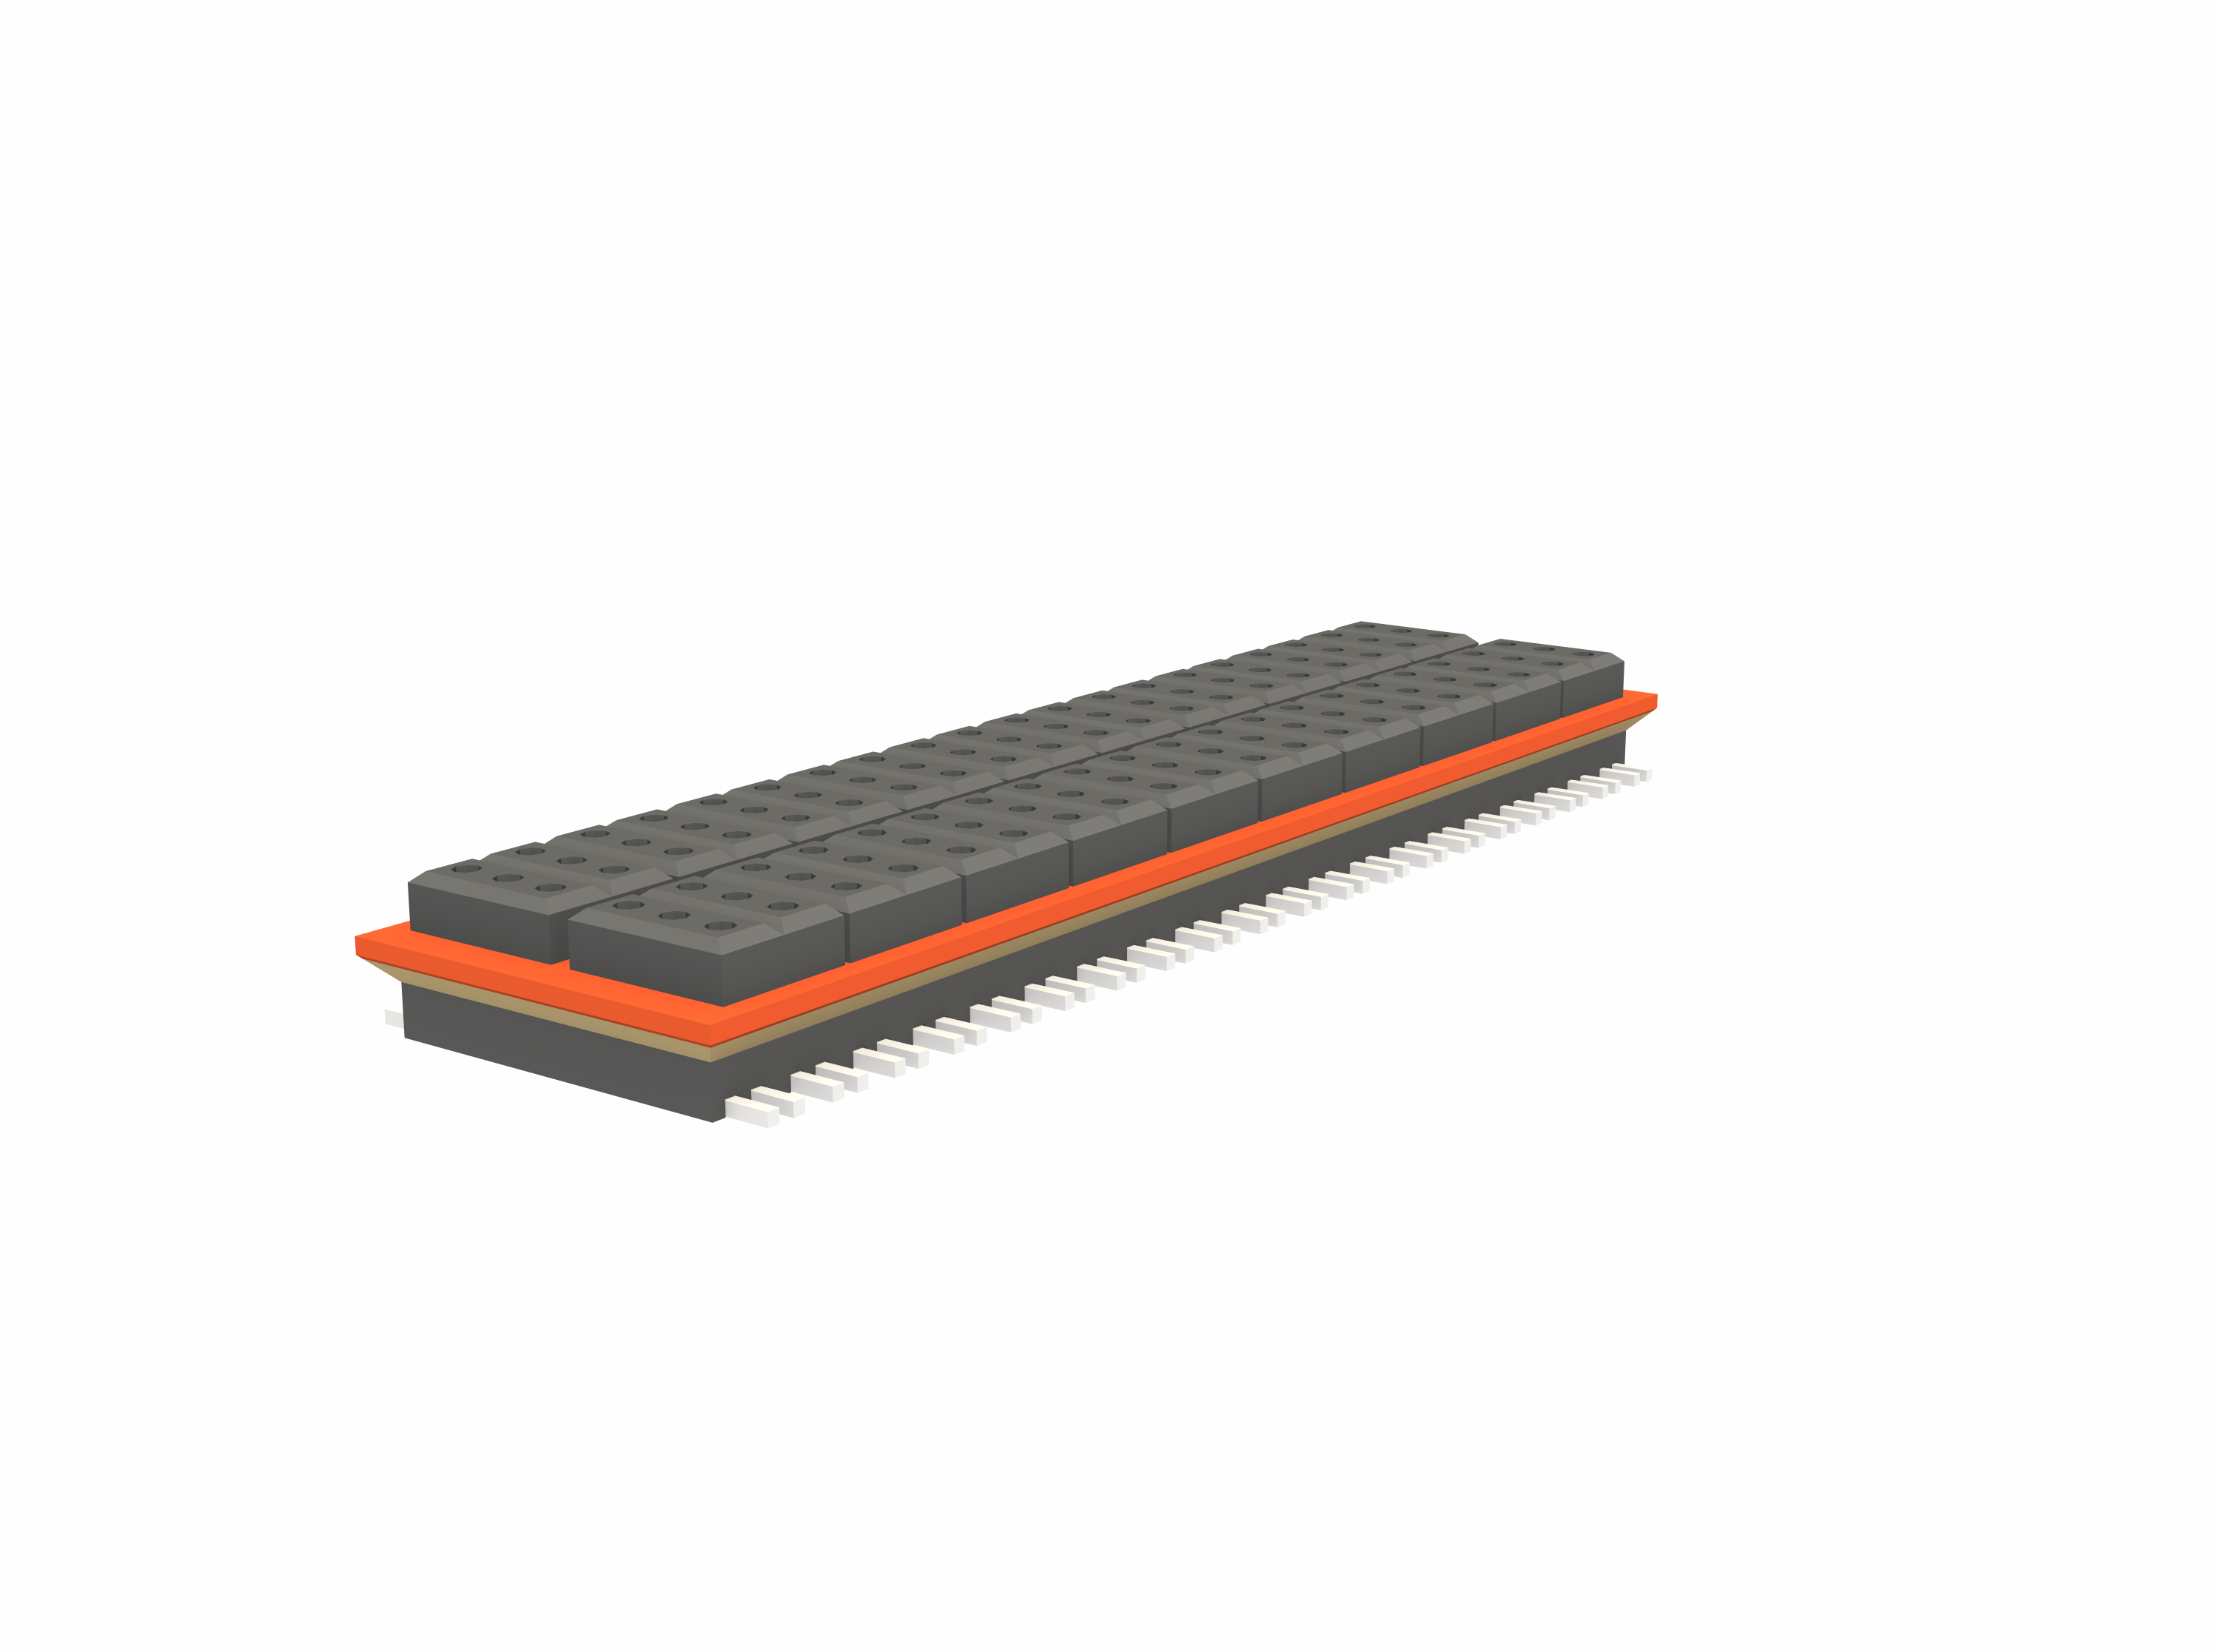
\includegraphics[width=\textwidth]{../media/populations/ap32-mesh-components/print/metal-bath-anodes-cathode-bus-bars.png}
      \caption{Éléments à proximité des fluides}
      \label{fig:ap32-geometry-elements}
    \end{subfigure}
%
    \begin{subfigure}[b]{0.49\textwidth}
      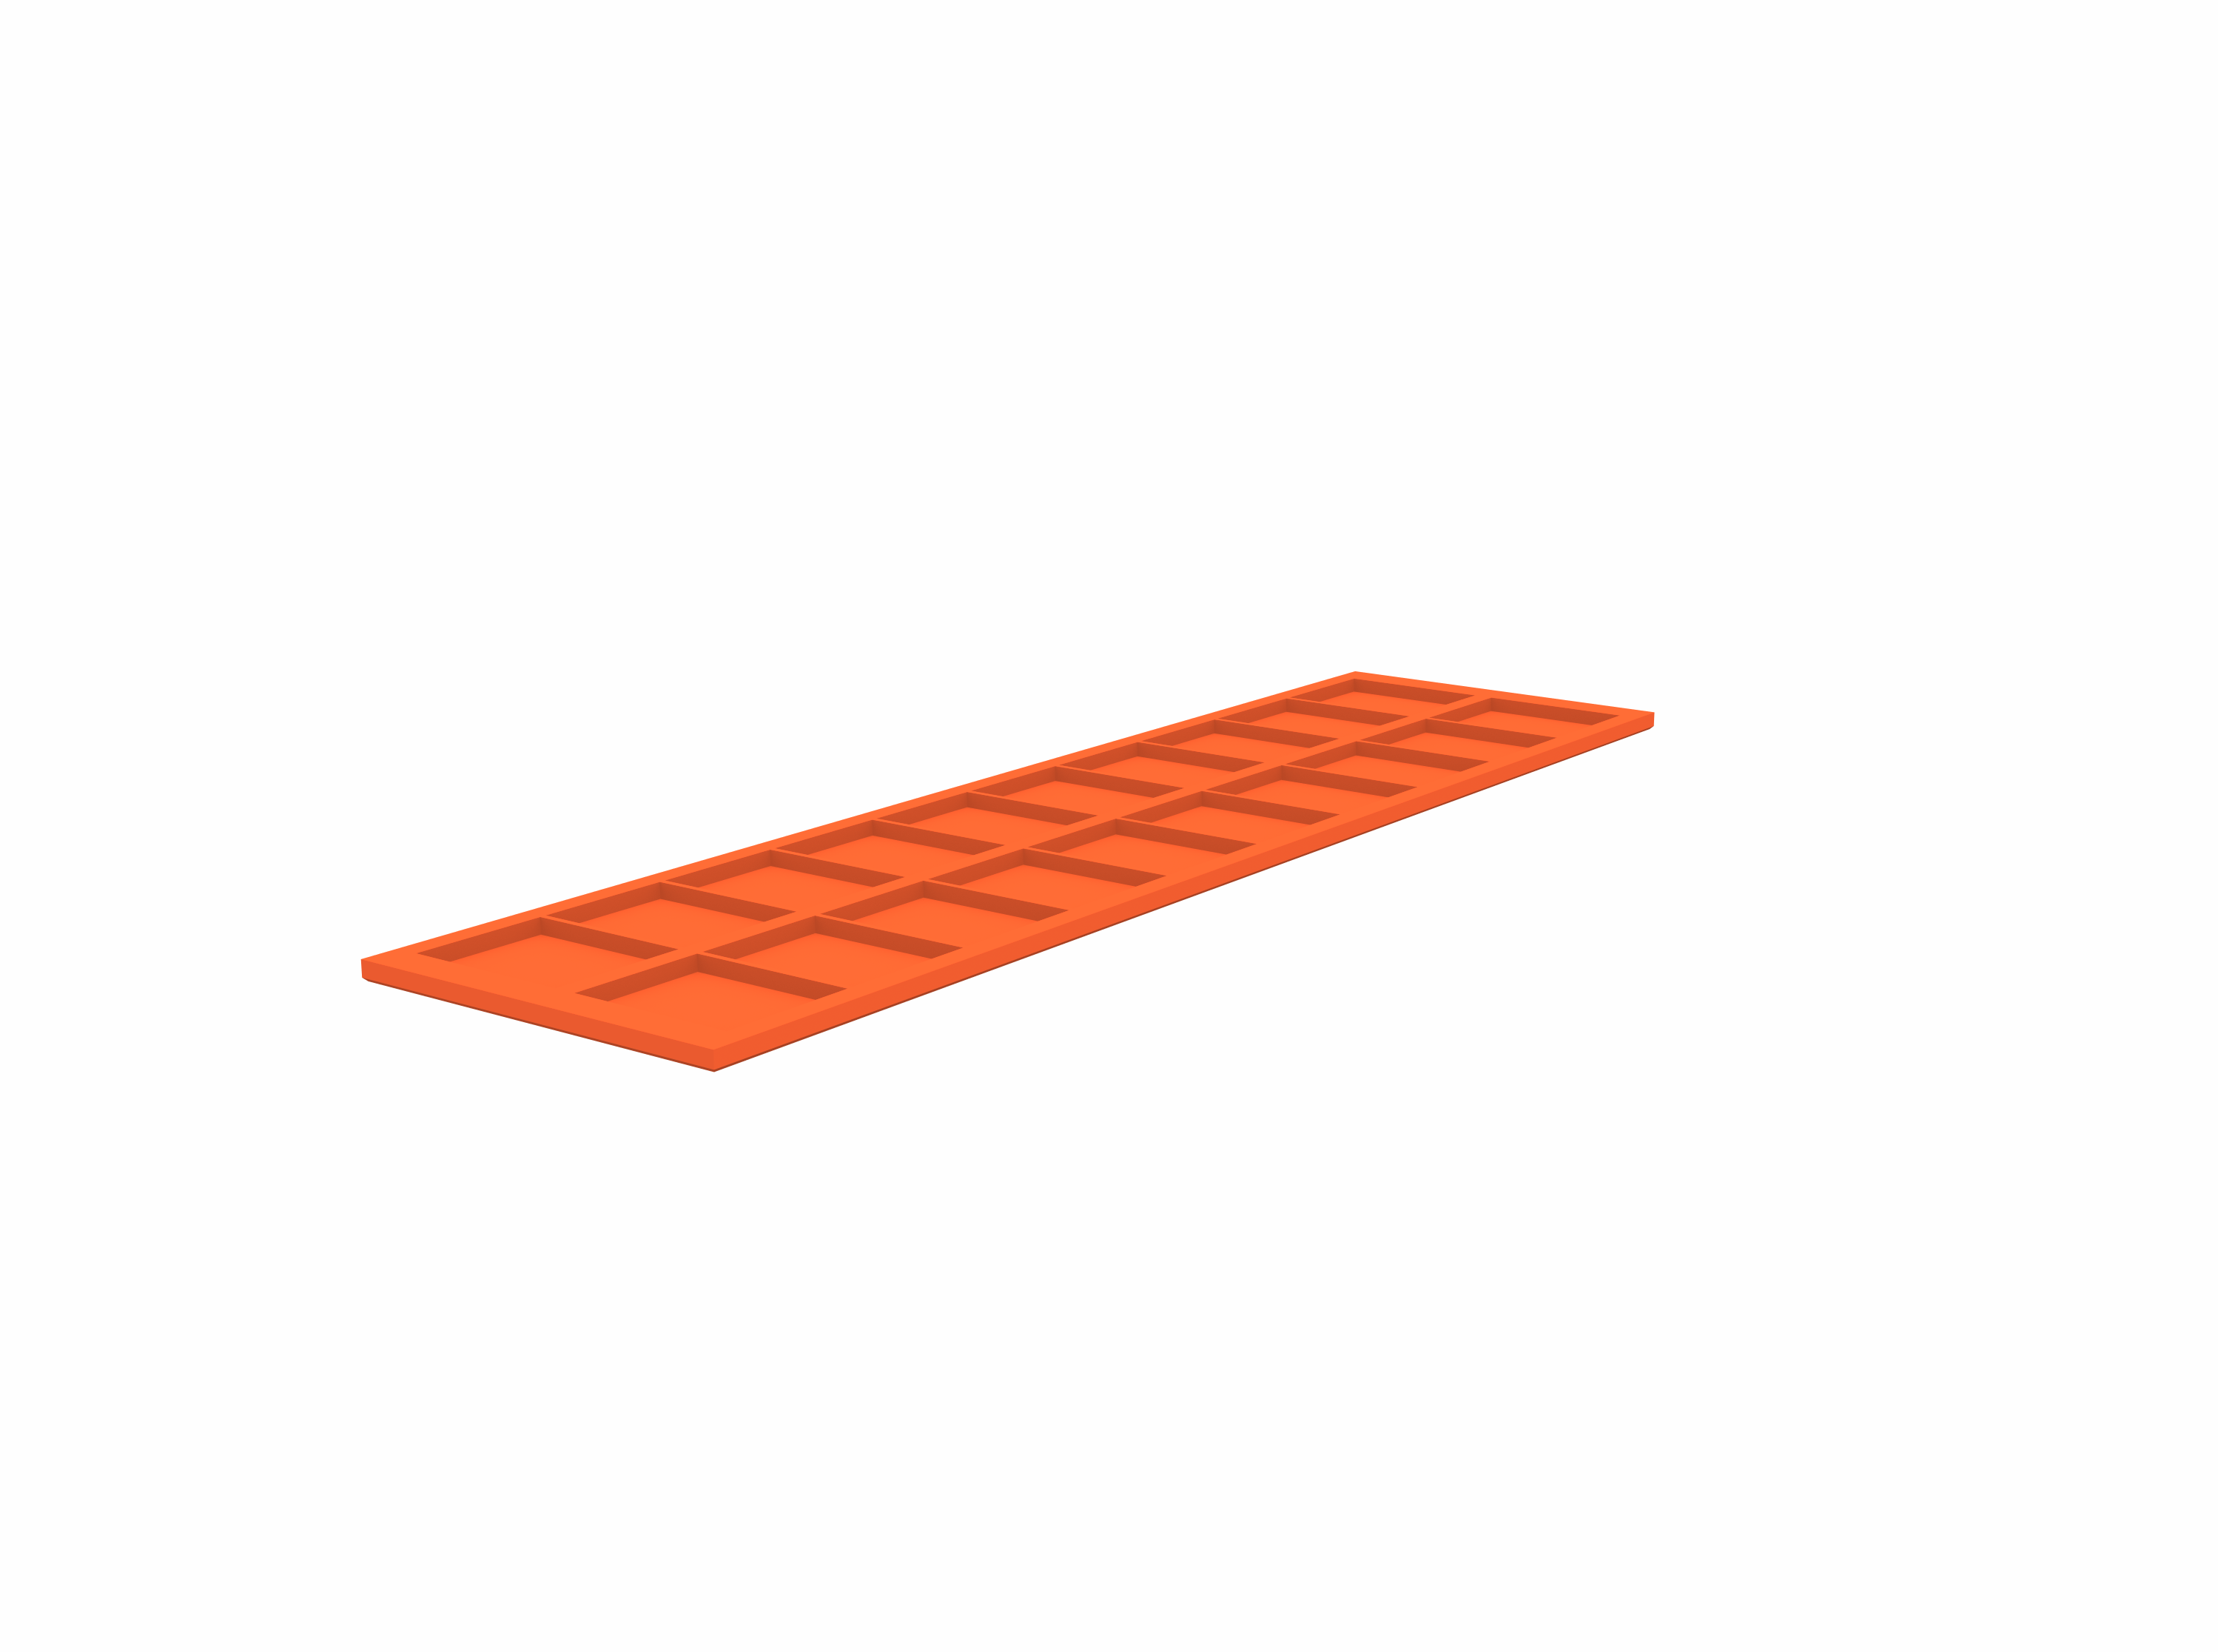
\includegraphics[width=\textwidth]{../media/populations/ap32-mesh-components/print/bath.png}
      \caption{Bain électrolytique}
      \label{fig:ap32-geometry-electrolyte}
    \end{subfigure}
%
    \caption{Géométrie des éléments importants à proximité
      du bain électrolytique dans une cuve AP32
      (fig. \ref{fig:ap32-geometry-elements}), et détail du volume
      occupé par le bain électrolytique dans cette même cuve
      (fig. \ref{fig:ap32-geometry-electrolyte}). On distingue les
      les anodes en haut et la cathode
      en bas (\textbf{noir}), le bain électrolytique
      (\textbf{orange}), le métal liquide (\textbf{jaune}) et les
      bus bar (\textbf{gris clair}).}
    \label{fig:ap32-geometry}
  \end{center}
\end{figure}

Le plan anodique est composée de deux rangées de 10 anodes chacune,
représentées en noir sur la figure \ref{fig:ap32-geometry-elements}. La
surface du plan anodique est d'environ \num{40.3} \si{\square\meter}
et seulement \num{25}\% de la surface du bain est libre, le reste
étant recouvert par les anodes. La cuve est conçue pour que
l'électrolyte soit traversé par un courant électrique total $I = $
\num{320000} \si{\ampere}, ce qui correspond à une densité de courant
d'environ \num{0.8} \si{\ampere\per\square\centi\meter} à la surface
des anodes. En supposant un rendement de réaction de \num{100}\%, ce
courant électrique permet de réduire par électrolyse \num{29.8}
\si{\gram\per\second} ou \num{2577.1} \si{\kilo\gram} par jour
d'aluminium métallique, \ie, un peu plus qu'\num{1} \si{\cubic\meter}
de métal par jour. Cet accroissement de volume de métal correspond à
une variation de l'épaisseur du métal liquide d'environ \num{2}
\si{\centi\meter}.

Du coté des anodes, la réaction d'électrolyse produit environ
\num{0.8} \si{\mol\per\second} d'oxygène \ce{O2}. Cet oxygène réagit
immédiatement avec le carbone de l'anode pour former du \ce{CO2}. Dans
l'ensemble de la cuve, l'électrolyse produit au total environ \num{80}
\si{\liter} par seconde de gaz, qui remonte vers la surface du bain
par le canal central et les canaux latéraux. La réaction de l'oxygène
avec le carbone des anodes provoque l'érosion de celles-ci à une
vitesse d'environ \num{1100} \si{\kilo\gram} par jour. Étant donné le
nombre total d'anodes et leur taille respectives, chaque anode d'une
cuve AP32 a une durée de vie d'environ 30 jours, après quoi elle doit
être remplacée par une anode neuve.

Pour compenser l'alumine dissoute qui est consommée par la réaction
d'électrolyse, il faut injecter en moyenne au cours du temps $56.3$
\si{\gram\per\second} de poudre d'alumine. Comme déjà mentionné dans
la section \ref{sec:introduction-hall-heroult}, la poudre d'alumine
est déposée à la surface du bain dans le canal central par une série
d'injecteurs dont la position est fixe. Un piqueur vient percer
mécaniquement un trou dans la croûte et créer un accès à la surface
libre du bain avant chaque injection. Ce trou se rebouche rapidement,
et pour cette raison l'injection de la poudre d'alumine ne peut pas
avoir lieu continûment.

Pour maintenir un rendement énergétique maximum, éviter l'émission de
gaz fluorés et éviter l'occurence des effets d'anodes, il est crucial
que la concentration d'oxyde d'aluminium dissout dans le bain soit
maintenue dans un intervalle très précis. Malheureusement, pour de
nombreuses raisons il est impossible de maintenir un bilan précis de
la quantité d'alumine dans le bain en fonction de ce qui est injecté
et de ce qui est consommé. En effet, l'environnement rend difficile la
pesée précise des quantités déposées, une partie des particules
volatiles ne parviennent jamais dans le bain, des agrégats se forme,
dont une partie s'accumule au fond de la cuve sur la cathode, et des
réactions chimiques parasites viennent, entre autres, grever ce bilan.

Pour contourner cette difficulté, les opérateurs exploitent le fait
que la resistivité du bain électrolytique dépend de la concentration
d'alumine dissoute, et atteint un minimum à la concentration optimale
$\concentration \approx$ \num{3}\% masse. En mesurant la chute de
potentiel électrique à travers le bain électrolytique, on maintient la
concentration d'alumine dissoute au voisinage de la concentration
optimale en alternant une phase de sur-alimentation en alumine et une
phase de sous-alimentation. Durant la phase de sur-alimentation, la
concentration d'alumine va passer au-delà de la concentration optimale
par conséquent accroître la resistivité du bain. Passé un certain
seuil, on débute une phase de sous-alimentation, durant laquelle la
résistivité commence par chuter, puis croît à nouveau. Passé un
certain seuil, on amorce une phase de sur-alimentation, et ainsi de
suite.

Dans chacune des phase de sur-alimentation ou sous-alimentation, les
injecteurs déposent les doses d'alumine selon une cadence préétablie
et périodique. La période et une taille des doses peut être spécifiée
indépendemment pour chaque injecteur.

\begin{figure}[t]
  \begin{center}
    \begin{tikzpicture}
      \begin{axis}[
          hide axis,
          colorbar,
          scale only axis,
          height=0.41\rasterimagewidth,,
          width=\rasterimagewidth,
          colorbar horizontal,
          point meta min=0.00,
          point meta max=0.05,
          colorbar style={
            title=Vitesse $u$ [\si{\meter\per\second}],
            width=7.4cm,
            height=0.3cm,
            xtick={0.00, 0.01, 0.02, 0.03, 0.04, 0.05},
            xticklabel style={
              /pgf/number format/fixed,
              /pgf/number format/fixed zerofill,
              /pgf/number format/precision=2
            },
            scaled x ticks = false,
            at={(0.5\rasterimagewidth,0.4cm)},
            anchor=north
          }
        ]
        \addplot [] coordinates {(0,0)};
        \node (myfirstpic) at (0,0) {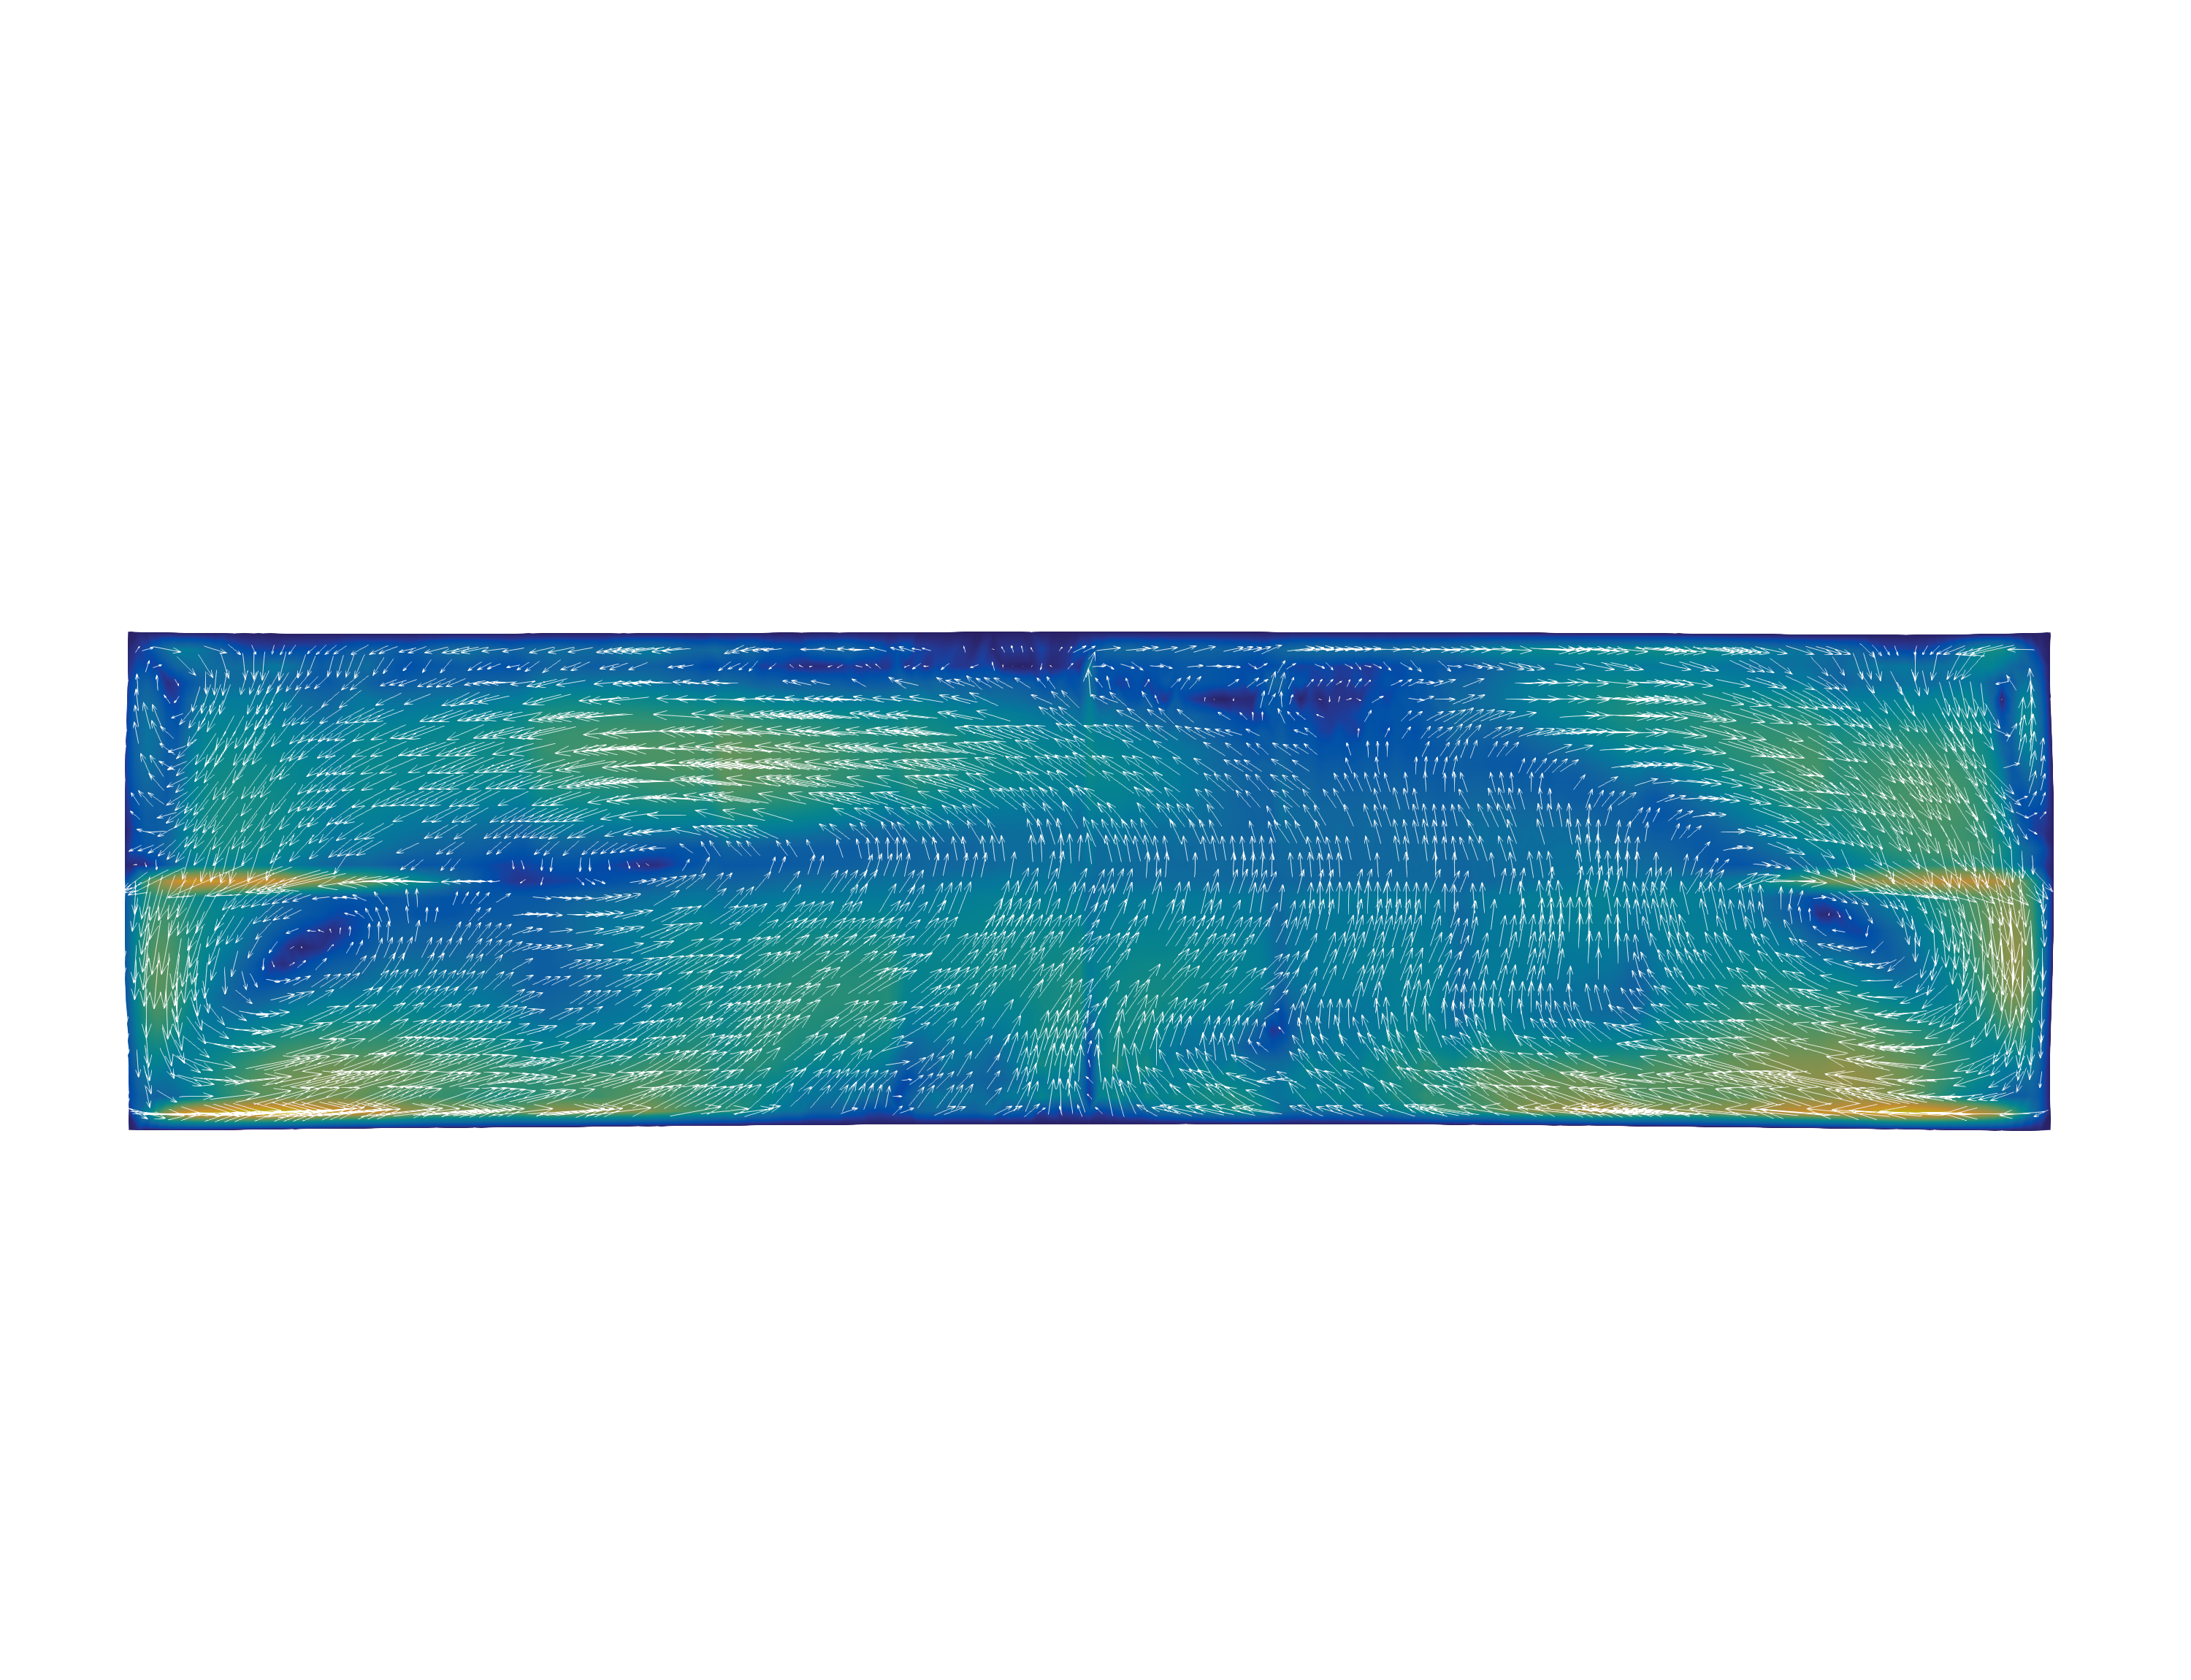
\includegraphics[width=\rasterimagewidth]{{../media/populations/ap32-fluid-flow/print/acd-all-anodes-velocity-0.00-0.05}.png}};
      \end{axis}
    \end{tikzpicture}
    \caption{Champ de vitesse $u$ dans le bain électrolytique d'une
      cuve AP32 restreint sur une surface placée à mi-hauteur de
      l'ACD, vue depuis dessus. Cette situation correspond à un état
      d'opération standard.}
    \label{fig:ap32-flow-acd}
  \end{center}
\end{figure}

\begin{figure}[t]
  \begin{center}
    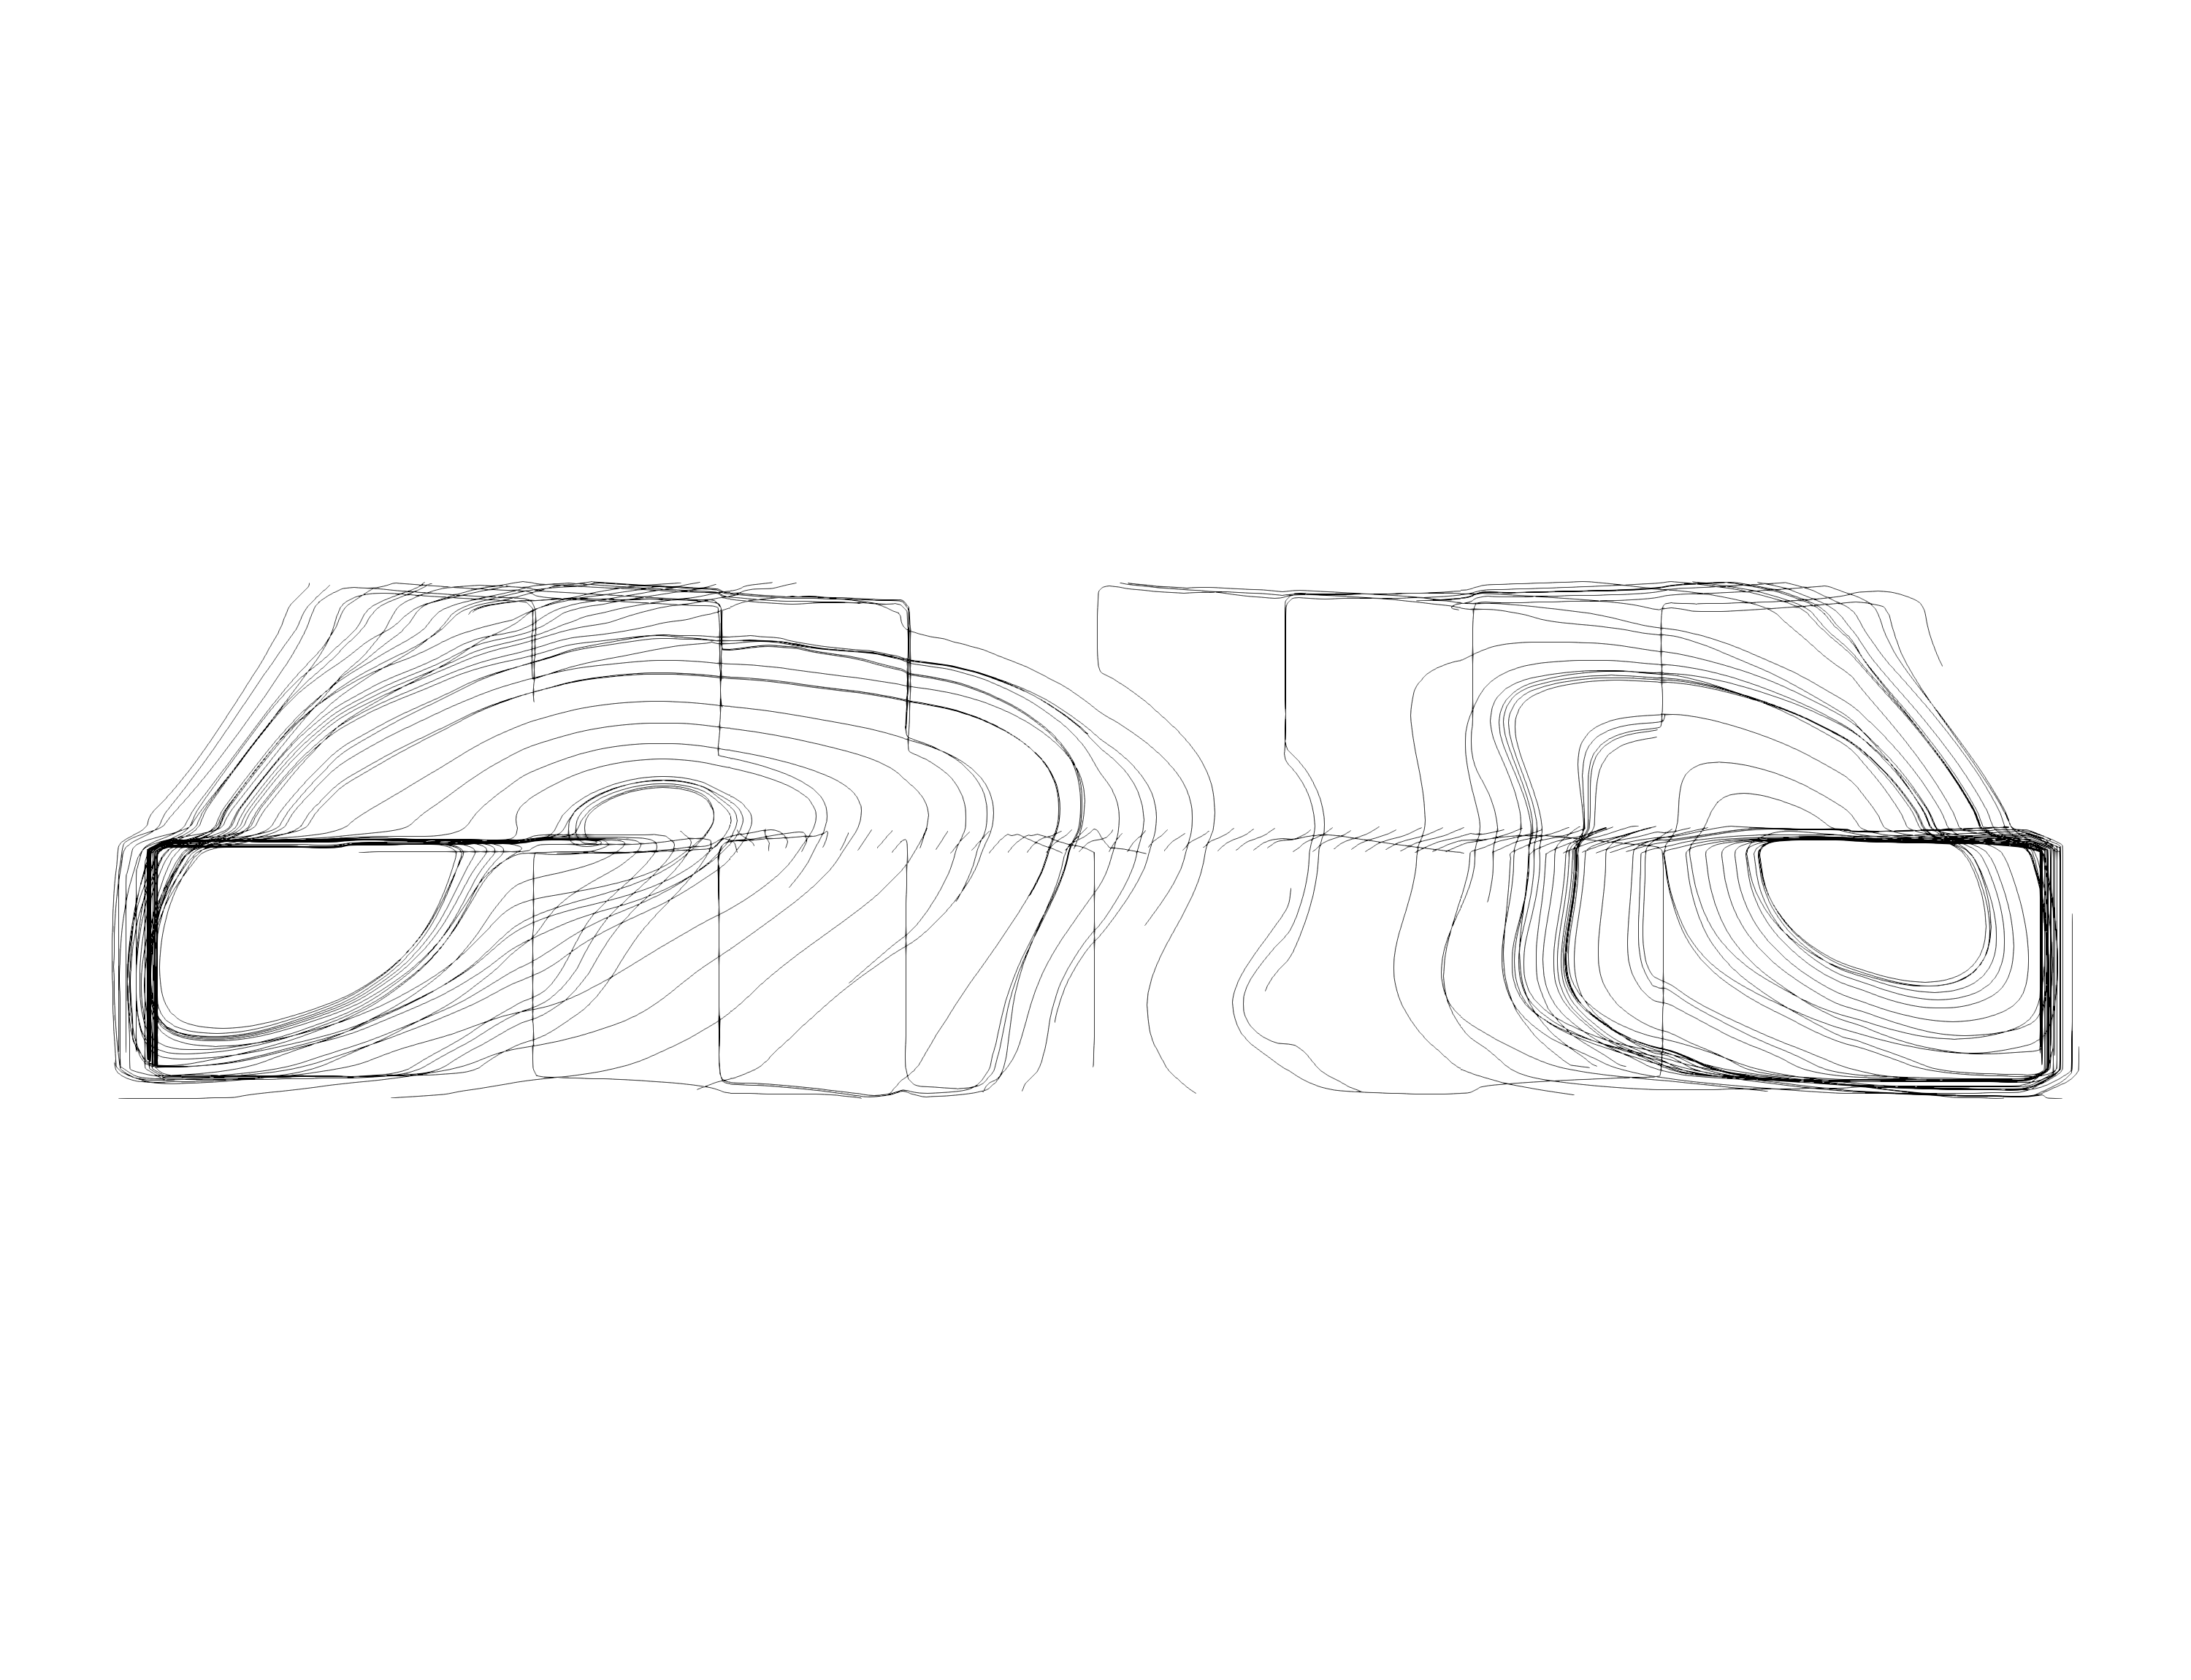
\includegraphics[width=\rasterimagewidth]{../media/populations/ap32-fluid-flow/print/chanel-velocity-streamlines.png}
    \caption{Lignes de courant correspondant au champ de vitesse
      représenté sur la figure \ref{fig:ap32-flow-acd}. Les lignes de
      courant prennent leur origine le long du canal central.}
    \label{fig:ap32-flow-streamlines}
  \end{center}
\end{figure}

\paragraph{Calcul de l'écoulement dans le bain} Une approximation de vitesse
d'écoulement du bain $u$ et de la densité de courant $j$ dans la cuve
AP32 est obtenue par l'intermédiaire du modèle multi-physique
stationnaire proposé par S. Steiner \cite{Steiner2009}, J. Rochat
\cite{Rochat2016} déjà introduit dans la section
\ref{sec:populations-introduction}. La figure \ref{fig:ap32-flow-acd}
représente la vitesse d'écoulement ainsi calculée par le logiciel
Alucell dans le bain électrolytique de la cuve AP32, dans
l'ACD. Lorsque la densité de courant électrique est répartie
uniformément sur toutes les anodes, l'écoulement dans les fluides
forme deux tourbillons principaux qui tournent en sens opposés. Deux
petits tourbillons se forment dans les coins avals. Les vitesse
maximales de l'écoulement (\num{5} \si{\centi\meter\per\second}
environ) sont atteinte dans le canal central au niveau des extrémités
de la cuve, ainsi que le long de la paroi amont, de part et d'autre de
la cuve. Dans le reste du bain et en particulier sous les anodes la
vitesse d'écoulement dépasse rarement \num{2}
\si{\centi\meter\per\second}. La figure
\ref{fig:ap32-flow-streamlines} illustre les lignes de courant de
l'écoulement dans le bain. On remarque les lignes de courant
s'engagent volontiers dans les canaux latéraux et dans le bain en
pourtour des rangées d'anodes.

\paragraph{Conditions sur l'injection et l'effet Joule}
Le schéma numérique proposé dans la section
\ref{sec:populations-discretisation} est conçu de manière à conserver
exactement d'une part la masse d'alumine dans les populations de
particules $\population$ et concentration d'alumine dissoute
$\concentration$, et d'autre part la quantité d'énergie thermique liée
à la température du bain $\temperature$. Pour des raisons déjà
évoquées, ces bilans ne sont pas exactement respectés dans une cuve
industrielle réelle, et il faut en général injecter un peu plus d'alumine
que ce qui est consommé par la réaction d'électrolyse. Quand à
l'énergie thermique, nous avons supposé que le bain est isolé
thermiquement, alors que dans une cuve réelle une quantité non
négligeable d'énergie s'échappe par le métal, les parois latérales de
la cuve, les anodes, la surface du bain et par le \ce{CO2} qui
s'échappe dans l'atmosphère.

Pour éviter que la masse totale d'alumine dans la cuve croisse sans
limite au cours du temps, il faut s'assurer que dans un état pseudo
stationnaire, la masse d'alumine reste proche de la masse d'alumine
initialement présente dans le bain. En d'autres termes, si $M_n$ est
la masse totale d'alumine dans le bain à l'instant $t_n$ telle que
définie dans la section (\ref{sec:populations-discretisation}), alors
on demande à ce que
\begin{equation*}
\lim_{n\to\infty} \frac{M_{n+1} - M_{0}}{t_n} = 0,
\end{equation*}
c'est-à-dire que
\begin{equation}\label{eq:injection-mass-condition}
  \frac{I[\cee{Al2O3}]}{6F}
  =\lim_{n\to \infty}\frac{1}{t_{n+1}}\ \sum_{\mathclap{\substack{k\\ p^k + 1\leq n +
        1}}}\ \int_\Omega\int_0^\infty\aluminadensity S^k \frac{4}{3}\pi r^3\intd{r}\intd{x}.
\end{equation}
Il faut donc choisir la masse des doses d'alumine injectées $S^k$, $k
= 1, 2,\dots$ et les temps d'injection $\tau^k$, $k = 1,2,\dots$ de
sorte à ce que le débit de masse de poudre d'alumine moyen au cours du
temps soit égal à $\frac{I[\cee{Al2O3}]}{6F}$, c'est-à-dire
\num{56.382e-3}\si{\kilo\gram\per\second}.

\begin{figure}
  \begin{center}
    \input{../media/populations/anode-configuration/anode-configuration.pdf_tex}
    \caption{Vue schématique de la partie supérieure du bain
      électrolytique. Les blocs rectangulaires représentent
      l'emplacement des anodes, tandis que les cercles indiqués par
      les flèches et numérotés marquent l'emplacement des injecteurs
      disposés le long du canal central.}
    \label{fig:anode-configuration}
  \end{center}
\end{figure}

La cuve AP32 possède 4 injecteurs placés au-dessus du canal central,
numérotés de 1 à 4, dans le sens de la coordonnée $x$ croissante (voir
la figure \ref{fig:anode-configuration}). Les paramètres qui
définissent chaque injecteurs sont regroupé dans la table
\ref{tab:injectors}.

\begin{table}
  \begin{center}
    \caption{Paramètres caractérisant les 4 injecteurs de la cuve AP32.}
    \label{tab:injectors}
    \begin{tabularx}{\textwidth}{@{}rrrrZ@{}}
      \toprule
      Injecteur & Position & Première injection & Intervalle d'injection & Masse de dose\\
      \midrule
      \#1         & \num{-4.4}\si\meter & \num{16}\si\second & \num{16}\si\second  & \num{0.225}\si{\kilo\gram} \\
      \#2         & \num{-1.6}\si\meter & \num{32}\si\second & \num{32}\si\second  & \num{0.451}\si{\kilo\gram} \\
      \#3         & \num{ 1.6}\si\meter & \num{48}\si\second & \num{48}\si\second  & \num{0.676}\si{\kilo\gram} \\
      \#4         & \num{ 4.4}\si\meter & \num{64}\si\second & \num{24}\si\second  & \num{0.338}\si{\kilo\gram} \\
      \bottomrule
    \end{tabularx}
  \end{center}
\end{table}
La masse des doses dans le tableau \ref{tab:injectors} est choisie de
telle sorte à ce que l'ensemble des 4 injecteurs injecte 25\% de la
masse d'alumine en moyenne. La forme des densité de particules
initiales $S^k$ est décrite dans \cite{Hofer2011}. Plus précisément,
la forme spatiale de chaque $S^k$ est une fonction lisse à support
compact centrée autour du point d'injection de l'injecteur
correspondant. La distribution en rayon initiale est approximée par
par une loi log-normale basée sur des mesures expérimentales. Puisque
le rapport des périodes d'injection des 4 injecteurs sont des nombres
rationnels, on peut définir une périodes globale liée à l'ensemble des
4 injecteurs. Étant données les périodes d'injections reportées dans le tableau
\ref{tab:injectors}, le cycle d'injection global est périodique après une
transition initiale de \num{64}\si\second, avec une période
de \num{192}\si\second. La figure \ref{fig:injections} représente les
injections qui ont lieu durant les \num{192} premières secondes de la
simulation.

\begin{figure}
  \begin{center}
    \input{../media/populations/cadence/cadence.tex}
    \caption{Temps d'injections des différents injecteurs de la cuve
      AP32. Chaque cercle représente une injection. Chaque ligne
      correspond à l'un des 4 injecteurs.}
    \label{fig:injections}
  \end{center}
\end{figure}

On détermine maintenant une condition sur la conductivité
électrique $\conductivity$, issue d'un argument similaire sur
l'énergie thermique du bain. Pour que l'énergie thermique du bain
reste proche de l'énergie thermique initiale, on demande à ce que
\begin{equation}
  \lim_{n\to\infty}\frac{\electrolytedensity\electrolytehc\displaystyle\int_\Omega\parent{\temperature_{n+1}
    - \temperature_0}\intd{x}}{t_{n+1}} = 0,
\end{equation}
ce qui correspond à la condition
\begin{eqnarray}
  \frac{1}{\conductivity} \int_\Omega j\cdot j\intd{x} &=&
  \aluminahc\parent{\tinit - \tinj}\lim_{n\to\infty}\frac{1}{t_{n+1}}\sum_{\mathclap{\substack{k\\ p^k +
  1 \leq n + 1}}}\int_\Omega\int_0^\infty\aluminadensity
  \frac{4}{3}\pi r^3 S^k\intd{r}\intd{x}\nonumber \\
  &&+
       {\aluminadissolutionenthalpy}\lim_{n\to\infty}\frac{1}{t_{n+1}}\sum_{m = 0}^{n}\sum_{\mathclap{\substack{k\\ q^k < m + 1}}} \int_\Omega\int_0^\infty \aluminadensity \frac{4}{3}\pi r^3\parent{n_{p,m+1}^k-n_{p,m}^k}\intd{r}\intd{x}\nonumber\\
       \label{eq:energy-condition}
\end{eqnarray}
en considérant (\ref{eq:energy-mass-balance}). Le premier terme du
membre de droite de (\ref{eq:energy-condition}) est égal à
\begin{equation*}
\aluminahc\parent{\tinit-\tinj}  \frac{I[\cee{Al2O3}]}{6F}
\end{equation*}
en vertu de (\ref{eq:injection-mass-condition}). Pour que le deuxième
terme du membre de droite de (\ref{eq:energy-condition}) converge, il
est suffisant que chaque population $k\geq 1$ se dissolve en un temps
fini donné quelque soit $k$. Plus précisément, les populations $n_p^k$
se dissolvent en un temps fini s'il existe un entier positif $q'$ tel
que $n_{p,n}^k = 0$ pour tout $n > q^k + q'$.

Le cas échéant on peut télescoper la somme sur $k$ et en remarquant que
\begin{equation*}
  \int_\Omega n_{p,q^k}^k\intd{x} = \int_\Omega S^k\intd{x}
\end{equation*}
pour tout $k \leq 1$ et pour tout $r > 0$ lorsque la vitesse de chute
$w = 0$, le deuxième terme du membre de droite de
(\ref{eq:energy-condition}) se réduit à
\begin{equation*}
  {\aluminadissolutionenthalpy}\lim_{n\to\infty}\frac{1}{t_{n+1}}\sum_{\mathclap{\substack{k\\ p^k +
  1 \leq n + 1}}}\int_\Omega\int_0^\infty\aluminadensity
  \frac{4}{3}\pi r^3 S^k\intd{r}\intd{x}.
\end{equation*}
Ainsi finalement,
\begin{equation*}
  \frac{1}{\sigma}\int_\Omega j\cdot j\intd{x}
  =\aluminahc\parent{\tinit-\tinj}\frac{I[\cee{Al2O3}]}{6F} + {\aluminadissolutionenthalpy}\frac{I[\cee{Al2O3}]}{6F}
\end{equation*}
et on fixe $\conductivity$ de sorte à satisfaire cette dernière
relation, c'est-à-dire que
\begin{equation}\label{eq:conductivity-condition}
  \conductivity = \frac{\displaystyle\int_\Omega j\cdot j\intd{x}}{\parent{\aluminahc\parent{\tinit-\tinj} + {\aluminadissolutionenthalpy} }
    \displaystyle\frac{I[\cee{Al2O3}]}{6F}}.
\end{equation}

\paragraph{Diffusivité du bain électrolytique} La vitesse d'écoulement
stationnaire du bain $u$ obtenue par la méthode introduite dans
\cite{Steiner2009}, \cite{Rochat2016} est la vitesse moyenne d'un
écoulement turbulent. Les structures turbulentes du fluide sont
décrites par un modèle de longueur de mélange de Smagorinsky
\cite{Rochat2016}. Dans le modèle de Smagorinsky, les structures
turbulentes de l'écoulement se traduise par une viscosité de
l'écoulement moyen $u$ proportionnelle au tenseur des déformation de
$u$. Dans le présent travail, nous caractérisons la diffusivité
$\electrolytecdiff$ de la concentration $\concentration$ et la
diffusivité $\electrolytetdiff$ de la température $\temperature$ par
deux réels $\electrolytemoldiff$, $\electrolyteturbdiff$ pour tout
$x\in\Omega$ de la manière suivante:
\begin{align}
  \electrolytetdiff(x) =  \electrolytecdiff(x) = \electrolytemoldiff +
  \electrolyteturbdiff\parent{2\sum_{i,j}\straintensor_{ij}(x)\straintensor_{ij}(x)}^{1/2},
\end{align}
où $\straintensor_{ij}$, $i, j = 1,2,3$ est le tenseur des déformation
de l'écoulement défini par
\begin{equation}
  \straintensor_{ij} = \frac{1}{2}\parent{\frac{\partial u_i}{\partial
      x_j} + \frac{\partial u_j}{\partial x_i}}.
\end{equation}
Les valeurs du paramètre $\electrolytemoldiff$, associé à la diffusion
moléculaire et de $\electrolyteturbdiff$, associé à la diffusion
induite par les turbulences de l'écoulement, sont rapporté dans le
tableau \ref{tab:dissolution-physical-parameters}.


\begin{table}
  \begin{center}
    \caption{Paramètres physiques et paramètres liés à la cuve AP32
      qui interviennent dans le transport et la dissolution de poudre
      d'alumine.}
    \label{tab:dissolution-physical-parameters}
    \begin{tabularx}{\textwidth}{@{}lllX@{}}
      \toprule
      Quantité                         & Valeur           & Unités                                      & Description \\
      \midrule
      $\electrolytedensity$            & \num{2130}       & \si{\kg\per\cubic\meter}                    & Masse volumique du bain électrolytique                          \\
      $\aluminadensity$                & \num{3960}       & \si{\kg\per\cubic\meter}                    & Masse volumique de l'oxyde d'aluminium                          \\
      $\electrolytehc$                 & \num{2945}       & \si{\joule\per\kilo\gram\per\kelvin}        & Chaleur spécifique du bain électrolytique liquide               \\
      $\aluminahc$                     & \num{1200}       & \si{\joule\per\kilo\gram\per\kelvin}        & Chaleur spécifique de l'oxyde d'aluminium                       \\
      $g$                              & \num{9.81}       & \si{\meter\per\square\second}               & Accélération de la gravité terrestre                            \\
      $I$                              & \num{320000}     & \si{\ampere}                                & Courant électrique total                                        \\
      $\faraday$                       & \num{96485.33}   & \si{\coulomb\per\mol}                       & Constante de Faraday                                            \\
      $\faradayyield$                  & \num{0.945}       & []                                          & Rendement de Faraday de l'électrolyse                           \\\relax
      [\ce{Al2O3}]                     & \num{0.102}      & \si{\kilo\gram\per\mol}                     & Masse molaire de l'oxyde d'aluminium                            \\
      $\tinit$                         & \num{1223}       & \si{\kelvin}                                & Température initiale du bain électrolytique                     \\
      $\tinj$                          & \num{423}        & \si{\kelvin}                                & Température d'injection des particules d'alumine                \\
      $\tliq$                          & \num{1218}       & \si{\kelvin}                                & Température du liquidus du bain électrolytique                  \\
      $\tcrit$                         & \num{1218.86}    & \si{\kelvin}                                & Température critique de dissolution dans le bain électrolytique \\
      $K$                              & \num{0.5e-09}    & \si{\square\meter\per\second}               & Taux de dissolution des particules d'alumine                    \\
      $\aluminadissolutionenthalpy$    & \num{5.3e5}      & \si{\joule\per\kilo\gram}                   & Enthalpie de dissolution de l'oxyde d'aluminium                 \\
      $\conductivity$                  & $\approx$ \num{900} & \si{\siemens\per\meter}                     & Conductivité électrique du bain électrolytique                  \\
%     $\electrolytelaminarviscosity$   & \num{2e-3}       & \si{\kilo\gram\per\meter\per\second}        & Viscosité laminaire du bain électrolytique                      \\
%     $\electrolyteturbulentviscosity$ & \num{2e-3}       & \si{\kilo\gram\per\meter\per\second}        & Viscosité turbulente du bain électrolytique                     \\
      $\electrolytemoldiff$            & \num{5e-4}       & \si{\squared\meter\per\second}              & Diffusivité moléculaire dans le bain                            \\
      $\electrolyteturbdiff$           & \num{5e-4}       & \si{\squared\meter\per\second}              & Diffusivité turbulente dans le bain                             \\
      $\electrolyteviscosity$          & \num{2e-3}       & \si{\kilo\gram\per\meter\per\second}        & Viscosité laminaire du bain électrolytique                      \\
      $\csat$                          & \num{1689.7}     & \si{\mol\per\cubic\meter}                   & Concentration de saturation de l'alumine dissoute               \\
      $\csatwp$                        & \num{7.8}        & w\%                                         & Concentration de saturation de l'alumine dissoute               \\
      $\cinit$                         & \num{635.3}      & \si{\mol\per\cubic\meter}                   & Concentration initiale de l'alumine dissoute                    \\
      $\cinitwp$                       & \num{3.0}        & w\%                                         & Concentration initiale de l'alumine dissoute                    \\
      \bottomrule
    \end{tabularx}
  \end{center}
\end{table}

\paragraph{Conditions initiales de la concentration et de la
  température}
Les conditions initiales des population de particules $n_p^k$ sont
données implicitement dans la description du modèle par la
relation (\ref{eq:splitting-np1-init}). Plus précisément, aucune
particule n'est présente dans le bain électrolytique à $t = 0$, et
donc $n_p(0, x,r) = 0$ pour $r>0$ et $x\in\Omega$.

On observe expérimentalement sur des cuves d'électrolyse industrielles
que celle-ci atteigne un état stationnaire périodique lié à la période
du cycle d'injection après un temps caractéristique de transition. On
observe typiquement l'établissement de cet état périodique par
d'intermédiaire de mesures indirectes de la résistivité électrique de
la cuve. Par analogie, dans le cadre du modèle de transport et
dissolution d'alumine nous nous attendons à ce que la densité de
particules $n_p$, la concentration $\concentration$ et la température
$\temperature$ atteigne asymptotiquement lorsque $t\to\infty$ un état
périodique stationnaire de période $P$ identique à la période du
cycle d'injection global, soit \num{192}\si{\second} dans notre cas.

Il est clair que plus les conditions initiales pour $c$ et
$\temperature$ sont éloignées de l'état périodique stationnaire
asymptotique, plus le temps nécessaire pour atteindre un tel état est
long. Par conséquent, nous choisissons des conditions initiales
uniformes en espace pour la concentration et la température, et qui
soient égales aux conditions optimales d'opération de la cuve AP32:
\begin{align*}
  & \concentration(0, x) = \cinit,\quad\forall x\in\Omega,\\
  & \temperature(0, x) = \tinit,\quad\forall x\in\Omega.
\end{align*}
Le paramètre $\tinit$ est reporté dans la table
\ref{tab:dissolution-physical-parameters}. La concentration initiale
$\cinit$ en \si{\mol\per\cubic\meter} s'exprime en fonction de la
concentration initiale $\concentration_{\text{init},\%\mathrm w}$ en \% masse à
l'aide de la formule:
\begin{equation*}
  \cinit = \frac{\cinitwp \cdot
    100^{-1}}{\electrolytedensity[\cee{Al2O3}]\parent{1 - \cinitwp\cdot
      100^{-1}\parent{1 - \displaystyle\frac{\electrolytedensity}{\aluminadensity}}}}.
\end{equation*}
Nous exploiterons également cette dernière formule pour convertir les
valeurs du champ de concentration en \% masse lors de la visualisation
des résultats. Les deux valeurs de la concentration initiale selon les
unités physique sont rapportées dans la table
\ref{tab:dissolution-physical-parameters}.
% paramètres numérique. (deltat, maillage, deltar, N_r)

\begin{figure}[t]
  \begin{center}
    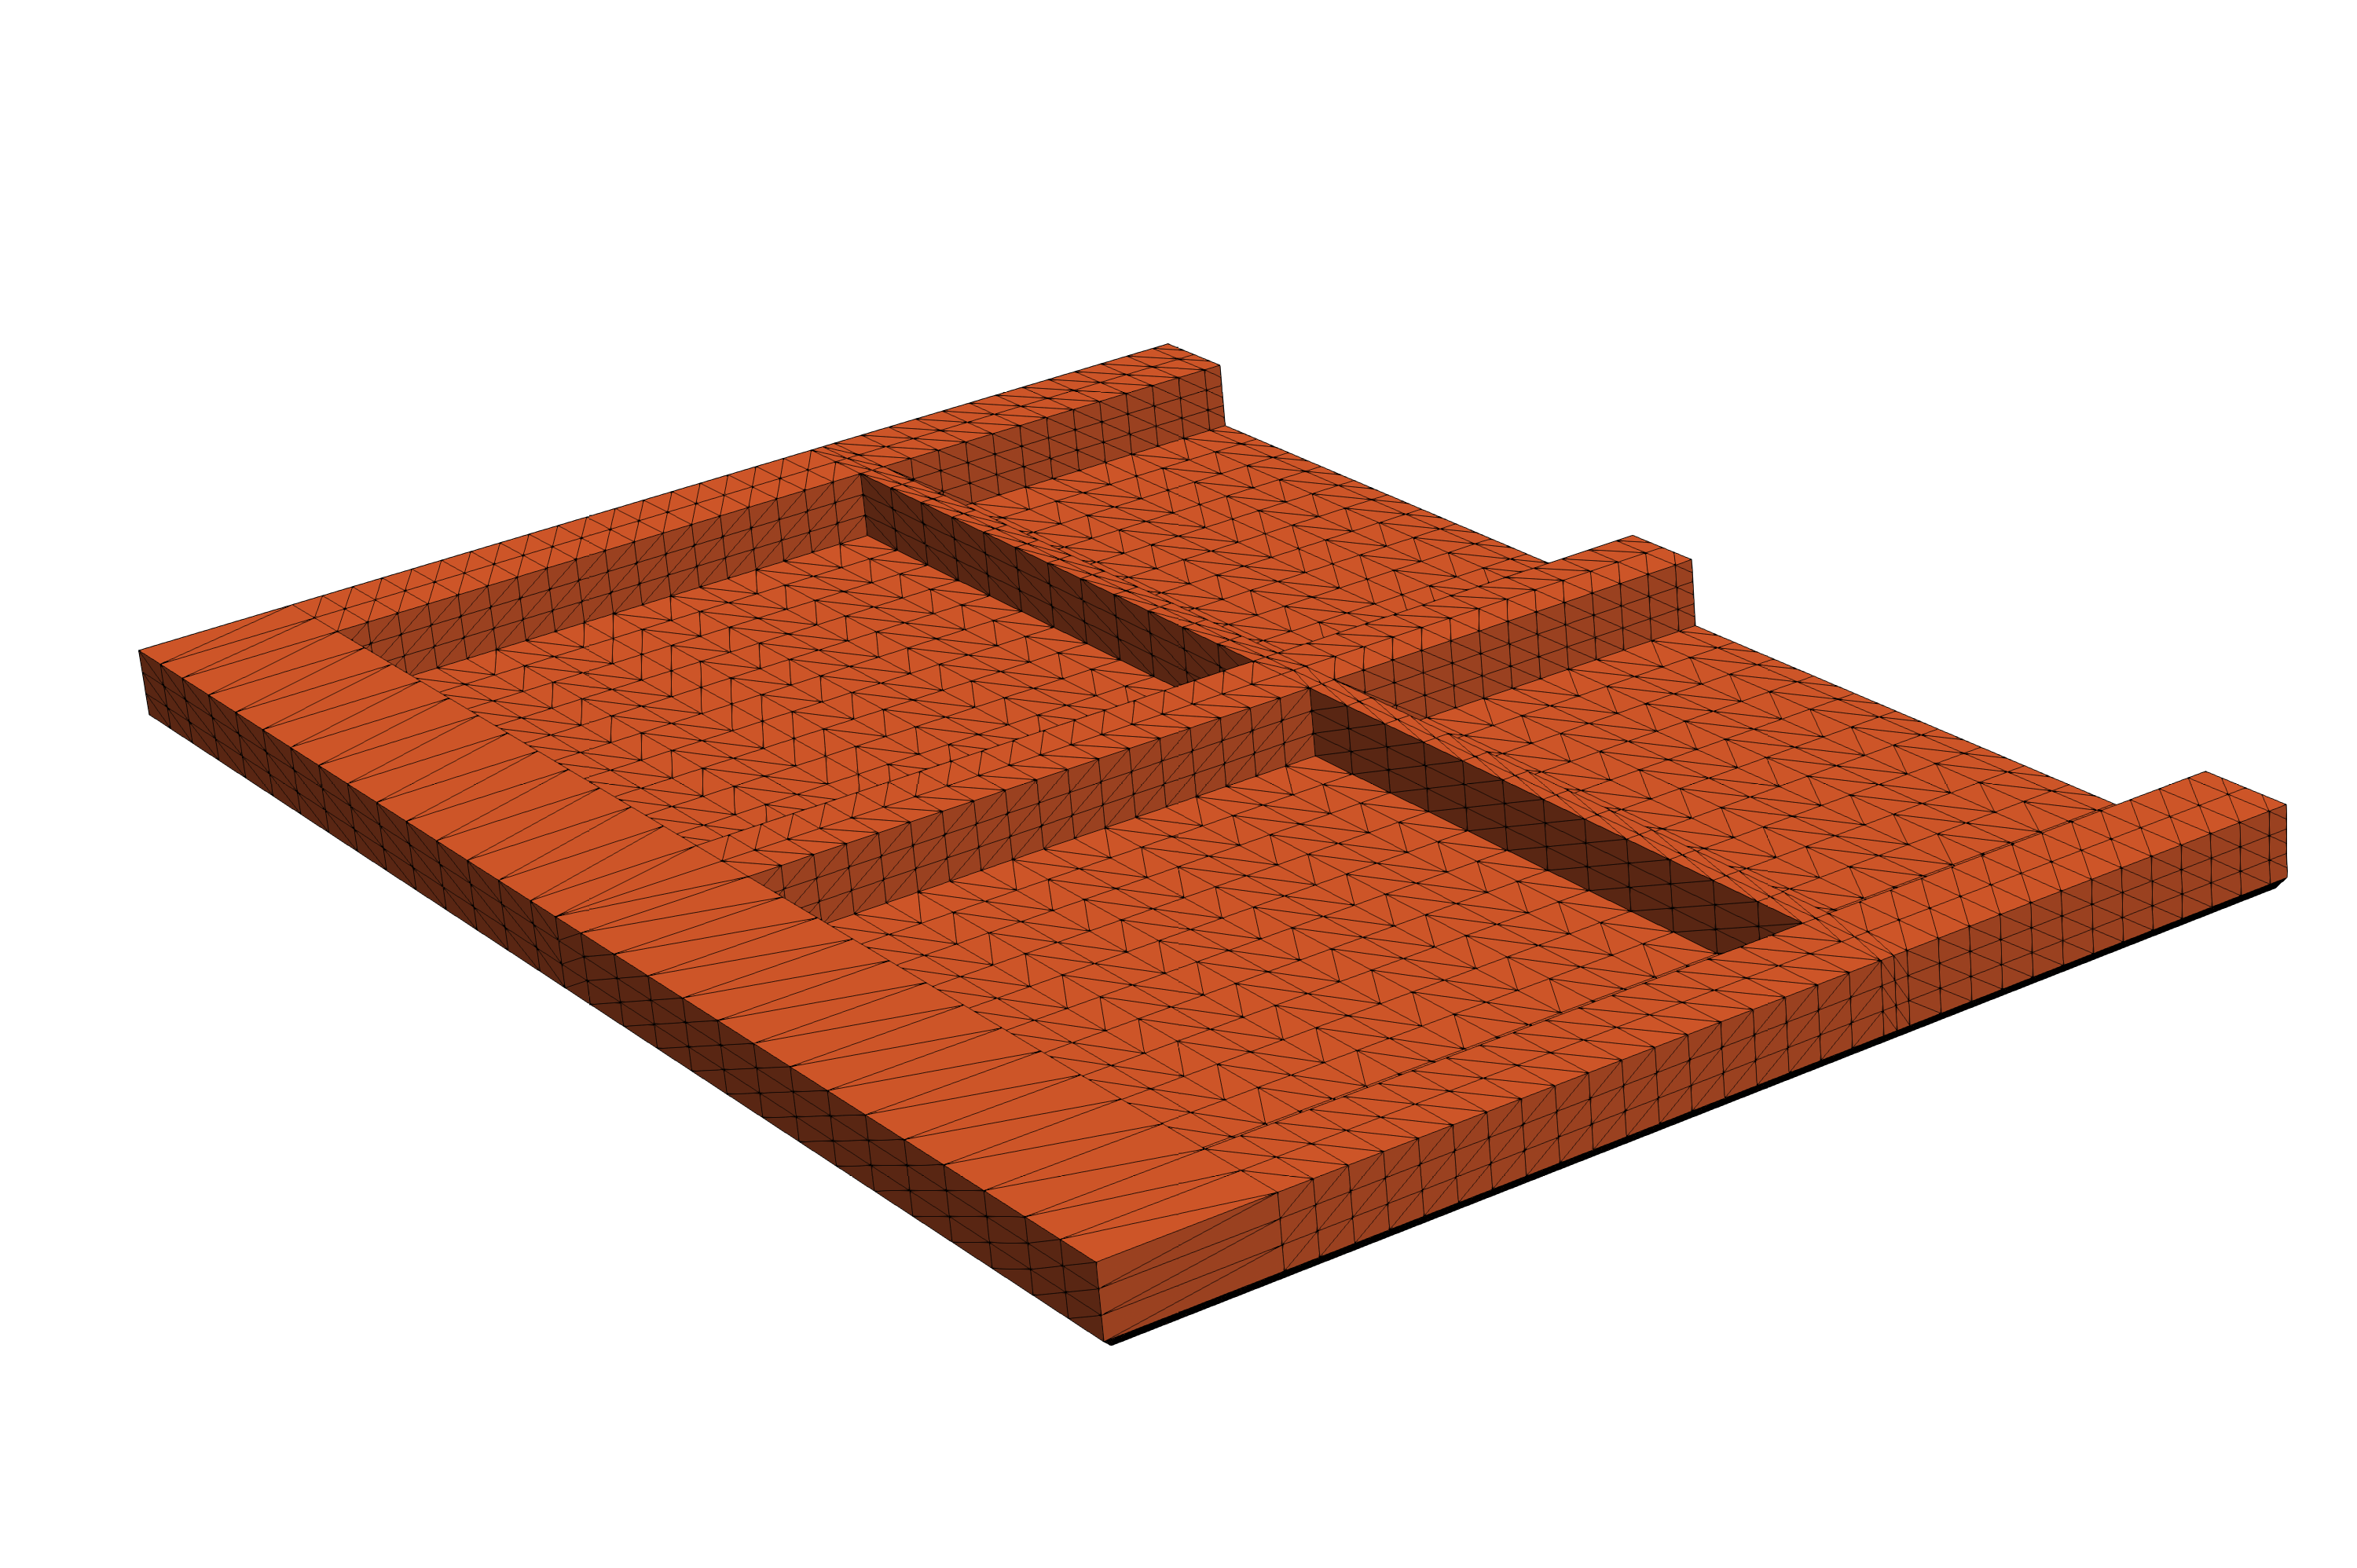
\includegraphics[width=\rasterimagewidth]{../media/populations/ap32-mesh-components/print/bath-mesh.png}
    \caption{Aperçu du maillage du domaine occupé par le bain
      électrolytique dans la cuve AP32.}
    \label{fig:bath-mesh}
  \end{center}
\end{figure}

\paragraph{Paramètres de discrétisation}
Le maillage du domaine $\Omega$ est obtenu en même temps que les
champs $u$ et $j$ par la méthode déjà évoquée plus haut proposée par
\cite{Steiner2009}, \cite{Rochat2016}. On peut voir sur la figure
\ref{fig:bath-mesh} un aperçu du maillage de $\Omega$ qui correspond à
l'une des extrémités de la cuve. Le maillage est fortement anisotrope,
avec des rapports d'aspect d'environ \num{25} dans l'ACD. Le diamètre
des mailles est compris entre \num{38}\si{\centi\meter} (aux
extrémités de la cuve) et \num{9}\si{\centi\meter} (dans l'ACD et les
canaux). Le maillage comporte \num{282240} éléments tetraédriques. On
choisit le nombre de discrétisation des rayons des particules $M = 5$
et $\dr = \num{40}$ \si{\micro\meter}. Enfin on fixe $\dt = 1$
\si{\second} et $T = \num{10000}$ \si{\second}, le temps auquel on
veut évaluer la concentration.


\paragraph{Solution de référence} Afin d'évaluer l'effet de la
température de l'électrolyte sur la dissolution de la poudre
d'alumine, nous commençons par présenter un calcul pour lequel les
particule d'alumine ne chute pas dans le bain, \ie, $w = 0$, pour
lequel les particules commencent à se dissoudre instantanément,
c'est-à-dire que $\tlat = 0$, et pour lequel la
vitesse de dissolution ne dépend pas de température du bain
$\temperature$. Plus précisément, la vitesse de dissolution définie
par (\ref{eq:dissolution-rate}) est remplacée par
\begin{equation}
  \dissolutionrate(c, \temperature)= \left\{
  \begin{array}{ll}
    K\displaystyle\frac{\csat - \concentration}{\csat} &\quad \text{si } 0\leq
    \concentration \leq \csat,\\
    0& \quad \text{sinon}.
  \end{array}
  \right.
\end{equation}
Cette situation est équivalente à supposer que la température du
bain $\temperature$ reste largement supérieure à la température
critique $\tcrit$ au cours du calcul, de sorte à ce que le terme
exponentiel dans (\ref{eq:dissolution-rate}) soit proche de zéro.

Un des objectifs recherchés par les opérateurs de cuve
industrielles est de minimiser les écarts de concentration autour de
la concentration d'alumine dissoute optimale. Pour évaluer le champ
de concentration par rapport à cet objectif, nous proposons de
représenter la variance  du champ de concentration
$c$ dans $\Omega$ au cours du temps définie par:
\begin{equation}
  \Var_c(t) = \sqrt{\int_\Omega\parent{\concentration(t, x) - \bar \concentration(t)}^2\intd{x}},
\end{equation}
où $\bar \concentration$ est la moyenne de $\concentration$ sur
$\Omega$:
\begin{equation}
  \bar \concentration(t) = \frac{1}{\abs{\Omega}}\int_\Omega c(t, x)\intd{x}
\end{equation}
et $\abs{\Omega}$ est le volume de $\Omega$. Clairement, la situation
idéale où la concentration d'alumine est uniforme dans tout
l'électrolyte correspond à une variance de $\concentration$ nulle. A
l'inverse, plus $\concentration$ s'écarte de sa valeur moyenne, plus
sa variance est importante.

La valeur de $\Var_\concentration$ au cours du temps offre un moyen
d'évaluer si le système a atteint l'état stationnaire périodique
recherché. Bien entendu ce n'est qu'une condition nécessaire, la
variance d'une fonction stationnaire est elle-même stationnaire, mais
l'inverse n'est pas nécessairement vrai. En pratique on prend soins de
vérifier que la différence en norme $L^2$ à deux instants successifs
séparés par la période du cycle d'injection global $P$ est inférieure
à \num{1}\%. Pour tous les calculs présenté dans cette partie, la
solution satisfait ce critère pour $T = \num{10000}$ \si{\second}.

\begin{figure}
  \begin{center}
    \input{../media/populations/variances/variance-control.tex}
    \caption{Évolution de $\Var_\concentration$ au cours du temps sur
      l'intervalle $[0, T]$ dans le bain électrolytique de la cuve
      AP32 lorsque la température n'est pas prise en compte dans la
      vitesse de dissolution des particules.}
    \label{fig:alumin-control-var}
  \end{center}
\end{figure}

La figure \ref{fig:alumin-control-var} représente l'évolution de
la variance de la concentration au cours du temps. On remarque une
phase initiale lorsque $t\in[0,500]$, au cours de laquelle la variance
croît rapidement. Cette croissance ralenti quand la concentration
approche de l'état stationnaire, et à partir de $t \approx
\num{4500}$ \si{\second} nous pouvons considérer que la
concentration est dans un état stationnaire et périodique. Les
fluctuation de $\Var_\concentration$ que l'on peut observer sur la
figure \ref{fig:alumin-control-var} sont dues aux injections de poudre
d'alumine dans le bain. Immédiatement après l'injection, la
dissolution des particules provoque un accroissement rapide de la
concentration d'alumine dissoute localement autour du point
d'injection. Lorsque la dose est totalement dissoute, ce pique de
concentration est atténué par la diffusion de la concentration
dans l'électrolyte. Cet effet se traduit par un accroissement de la
variance de la concentration immédiatement après l'injection d'une
dose, puis par une décroissance de la variance.

Cependant, ces variations de la concentration dans l'état
stationnaire sont très localisées autour des points d'injection. Dans
le reste du bain électrolytique, les variations de la concentration
restent de l'ordre de \num{1}\%.

Puisque, lorsque l'état stationnaire périodique est atteint, la
concentration varie peu au cours du cycle d'injection global, nous
pouvons nous permettre de visualiser la distribution de la
concentration dans le bain électrolytique à un instant arbitraire du
cycle d'injection global. Le temps $T = \num{10000}$ \si{\second}
auquel la solution est évaluée correspond donc à environ \num{51}
périodes du cycle d'injection global, sans compter la phase
transitoire initiale de \num{64} \si{\second}.

\begin{figure}[h]
  \begin{center}
    \begin{tikzpicture}
      \begin{axis}[
          hide axis,
          colorbar,
          scale only axis,
          height=0.41\rasterimagewidth,,
          width=\rasterimagewidth,
          colorbar horizontal,
          point meta min=2.38,
          point meta max=4.21,
          colorbar style={
            title=Concentration $c$ [\%w],
            width=7.4cm,
            height=0.3cm,
            xtick={2.38, 2.50, 3.00, 3.50, 4.00, 4.21},
            xticklabel style={
              /pgf/number format/fixed,
              /pgf/number format/fixed zerofill,
              /pgf/number format/precision=2
            },
            scaled x ticks = false,
            at={(0.5\rasterimagewidth,0.4cm)},
            anchor=north
          }
        ]
        \addplot [] coordinates {(0,0)};
        \node (myfirstpic) at (0,0) {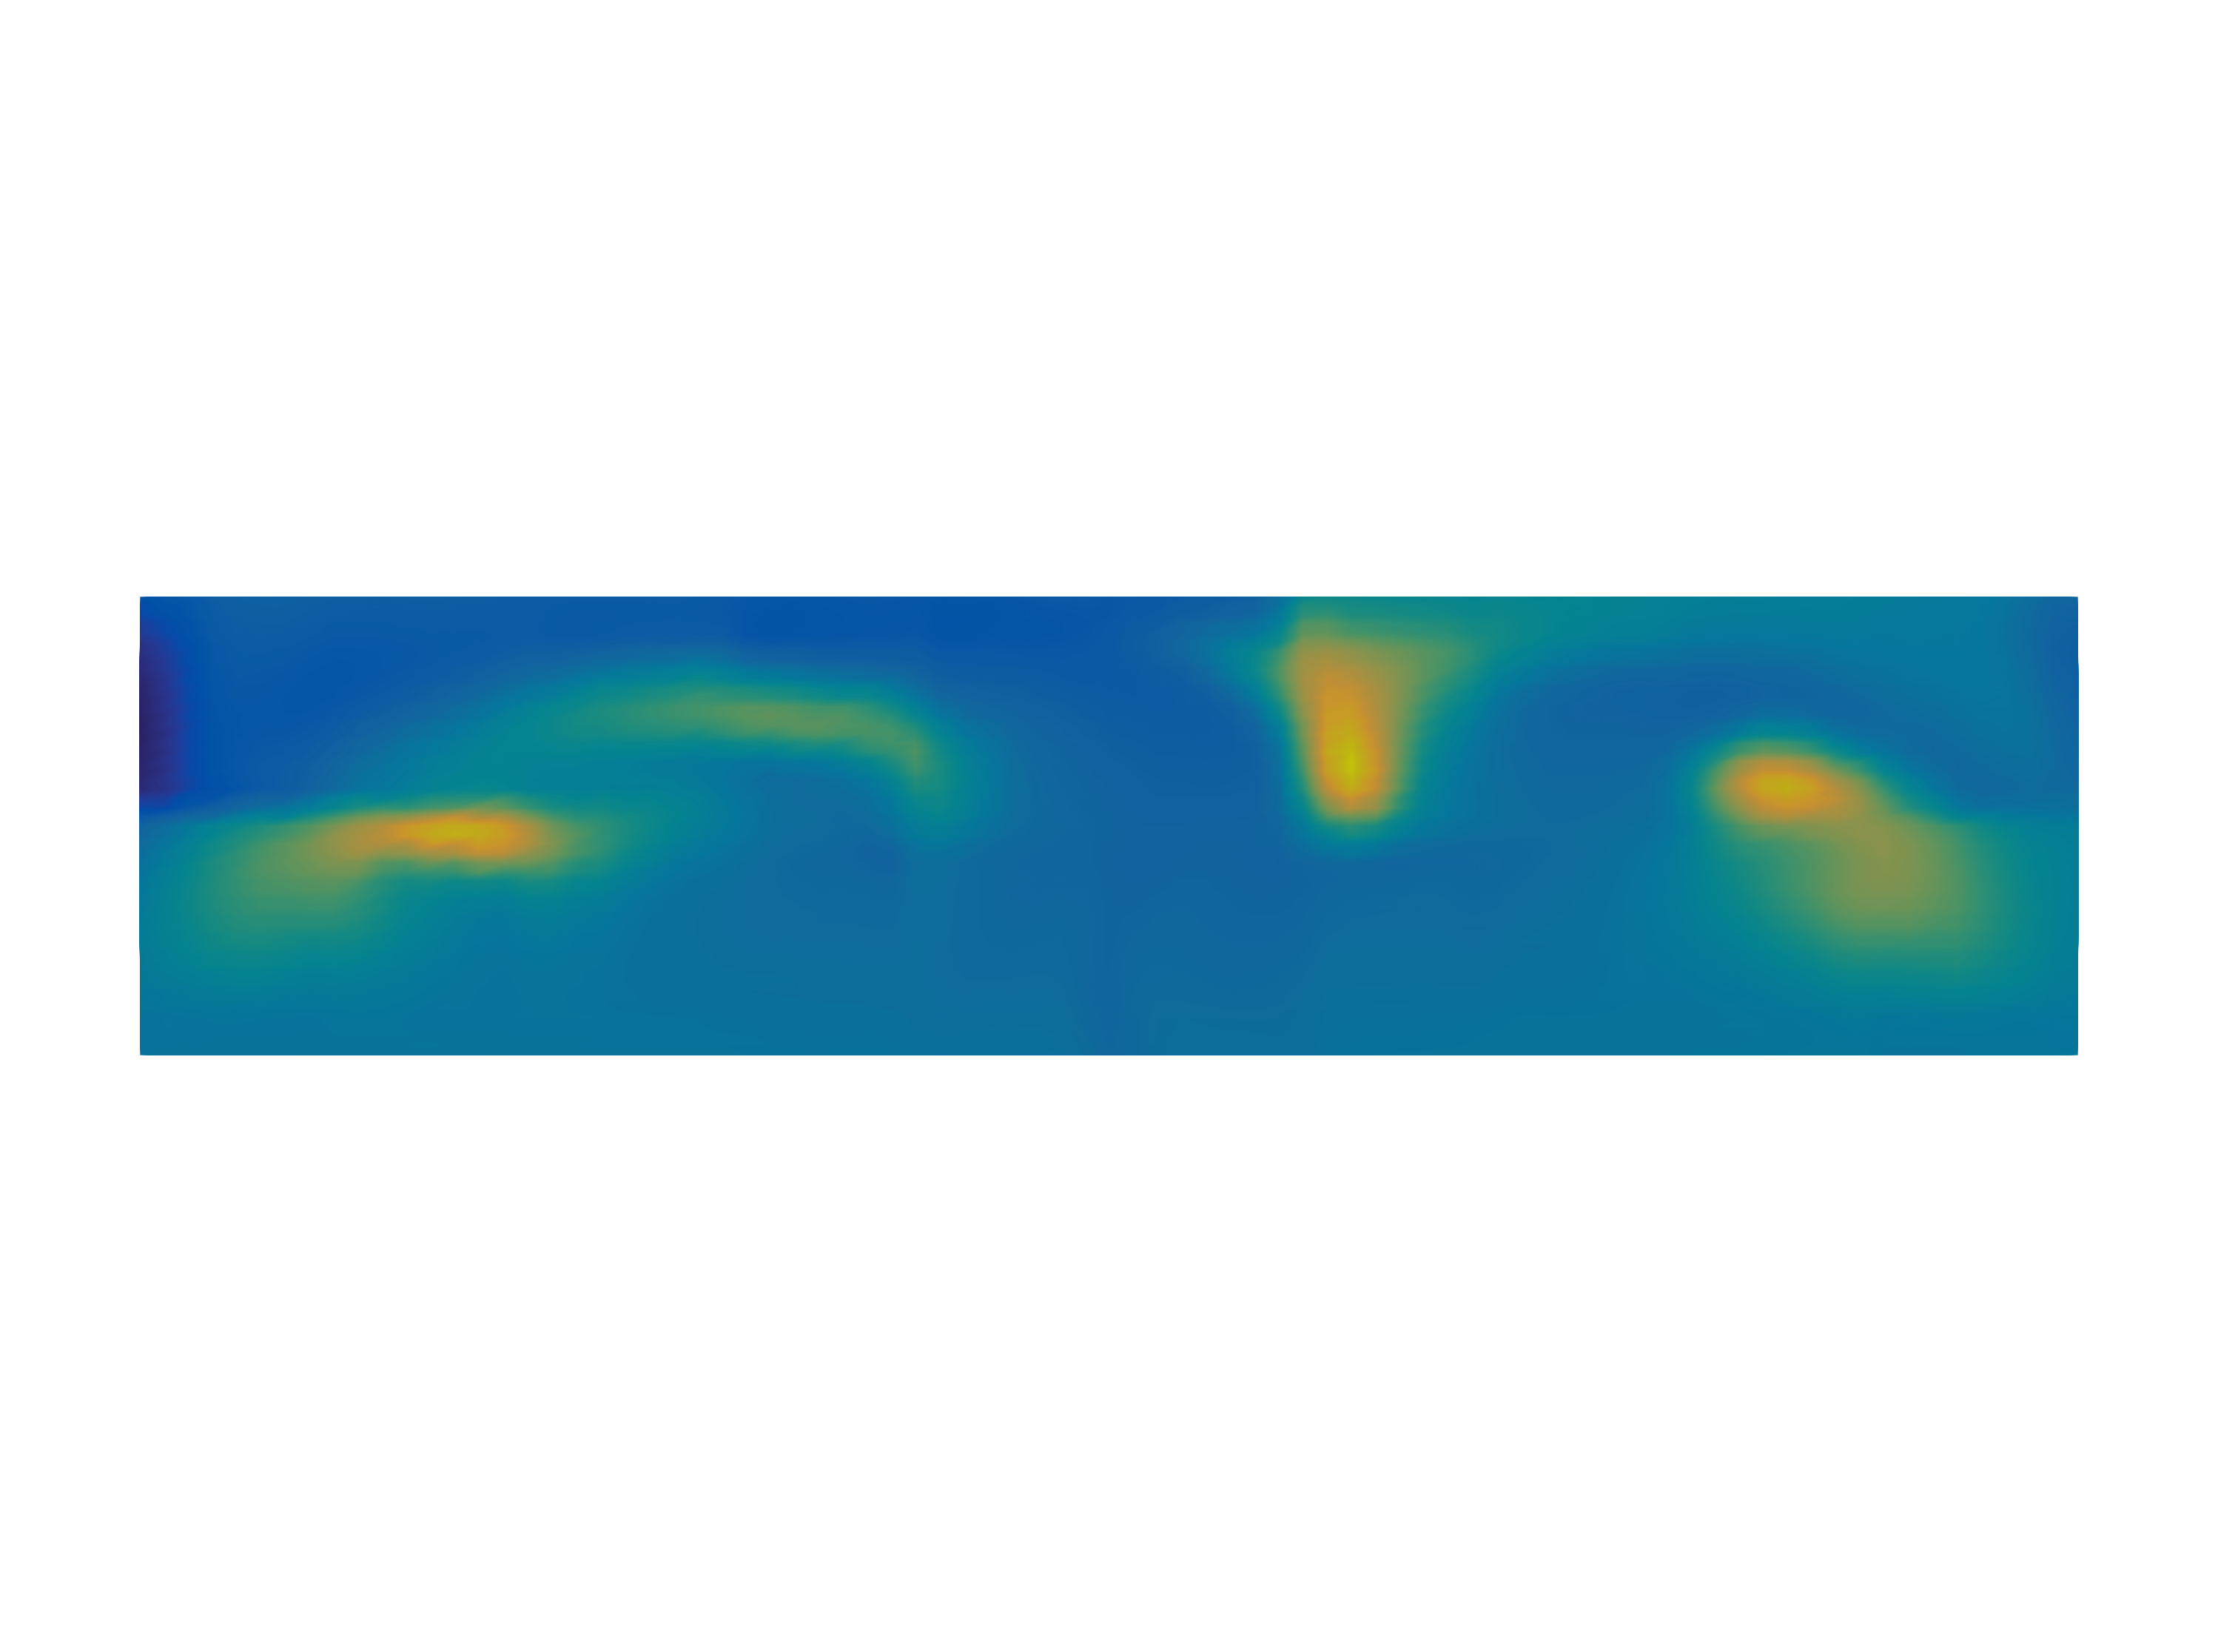
\includegraphics[width=\rasterimagewidth]{{../media/populations/application/print/alumina-control-2.38-4.21}.png}};
      \end{axis}
    \end{tikzpicture}
    \caption{Concentration d'alumine dissoute dans à $t =
      \num{10000}$ \si{\second} dans l'ACD de la cuve AP32, lorsque la
    température n'est pas prise en compte dans la vitesse de
    dissolution des particules.}
    \label{fig:ap32-alumina-wo-t}
  \end{center}
\end{figure}

On s'intéresse à la distribution de la concentration d'alumine là où a
lieu la réaction d'électrolyse, c'est-à-dire essentiellement dans
l'ACD. On se contente donc de visualiser la distribution de la
concentration d'alumine dans cette zone. Dans le domaine $\Omega$
occupé par l'électrolyte, l'ACD est maintenue constante avec $3.2$
\si{\centi\meter} d'épaisseur sur l'ensemble de l'interface. Pour
visualiser la concentration d'alumine dissoute dans l'ACD, on évalue
$\concentration$ sur une surface fictive placée dans l'électrolyte,
parallèle à l'interface et à une distance égale à la moitié de
l'ACD. La figure \ref{fig:ap32-alumina-wo-t} présente la distribution de la
concentration d'alumine dans le bain électrolytique.

On remarque sur la figure \ref{fig:ap32-alumina-wo-t} que la
concentration atteint des maximums locaux aux voisinages des points
d'injection, ce qui montre que l'essentiel de la poudre d'alumine se
dissout dans ces régions. Cette alumine dissoute est ensuite
transportée par l'écoulement. Les deux injecteurs de gauche alimentent
le tourbillon de gauche, tandis que les deux injecteurs de droite
alimentent essentiellement le tourbillon de droite. Les régions du bain
sous-alimentées sont les coins en aval, où la concentration descend
en dessous de \num{3} \%w et où l'écoulement est
caractérisé par la présence de petits tourbillons isolés. La région
centrale en amont des points d'injections est remarquablement uniforme
avec une concentration proche de \num{3} \%w.


Nous consacrons maintenant le reste de cette partie au
modèle de transport et dissolution d'alumine qui dépend de la
température du bain dans le bain de la cuve AP32, et l'on étudie
l'influence des nouveaux paramètres que ce modèle introduit,
en particulier le temps de latence $\tlat$, la température initial du
bain $\tinit$, la température critique $\tcrit$ et la vitesse de
chute des particules dans le bain $w$.


% Sensibilité par rapport a la latence de dissolution
\paragraph{Sensibilité par rapport au temps de latence}
Nous avons montré dans le paragraphe \ref{sec:particle-freeze} que le
temps de latence qui précède le début de la dissolution d'une
particule lâchée dans le bain d'une cuve d'électrolyse est de l'ordre
de \num{1e-1} \si{\second}. Ce temps caractéristique est
négligeable devant le temps de dissolution qui est au minimum de
\num{10} \si{\second} pour le choix de paramètres reportés dans la
table \ref{tab:dissolution-physical-parameters}.

Cependant, lors de l'injection d'une dose d'alumine typique, les
particules ne peuvent plus être suffisamment dispersées pour que
les hypothèses du modèle introduit dans la section
\ref{sec:particle-freeze} soient satisfaites, et c'est l'effet
collectif de l'ensemble des particules qui prédomine. Selon
\cite{Dassylva2015}, toutes les particules d'une dose subissent un
temps de latence de l'ordre de \num{1} \si{\second} quel que soit leur
taille.

Nous proposons maintenant de déterminer si la distribution de
concentration dans le bain électrolytique est sensible au temps de
latence de dissolution des particule lors de leur injection. Dans ce
but, nous présentons les résultats de 4 calculs du champ de
concentration d'alumine dissoute $c$ dans le bain électrolytique de
la cuve AP32 avec le modèle de transport et dissolution de
particules en fonction de la température du bain, avec les
paramètres reportés dans la table
\ref{tab:dissolution-physical-parameters} à l'exception du temps de
latence $\tlat$ pour lequel nous fixons successivement $\tlat = $
\numlist{1;2;5;10} secondes.

\begin{figure}[!hp]
  \begin{center}
      \begin{tikzpicture}
        \begin{axis}[
            %colorbar,
            hide axis,
            scale only axis,
            height=0.26\rasterimagewidth,,
            width=\rasterimagewidth,
            %colorbar horizontal,
            point meta min=2.54,
            point meta max=3.08,
            colorbar style={
              title=Concentration [\%w],
              width=7.4cm,
              height=0.3cm,
              xtick={2.54, 2.75 3, 3.08, 3.5, 4, 4.5, 5, 5.5, 6},
              at={(0.5\rasterimagewidth,0.4cm)},
              anchor=north
            }
          ]
          \addplot [] coordinates {(0,0)};
          \node (myfirstpic) at (0,0) {\framebox{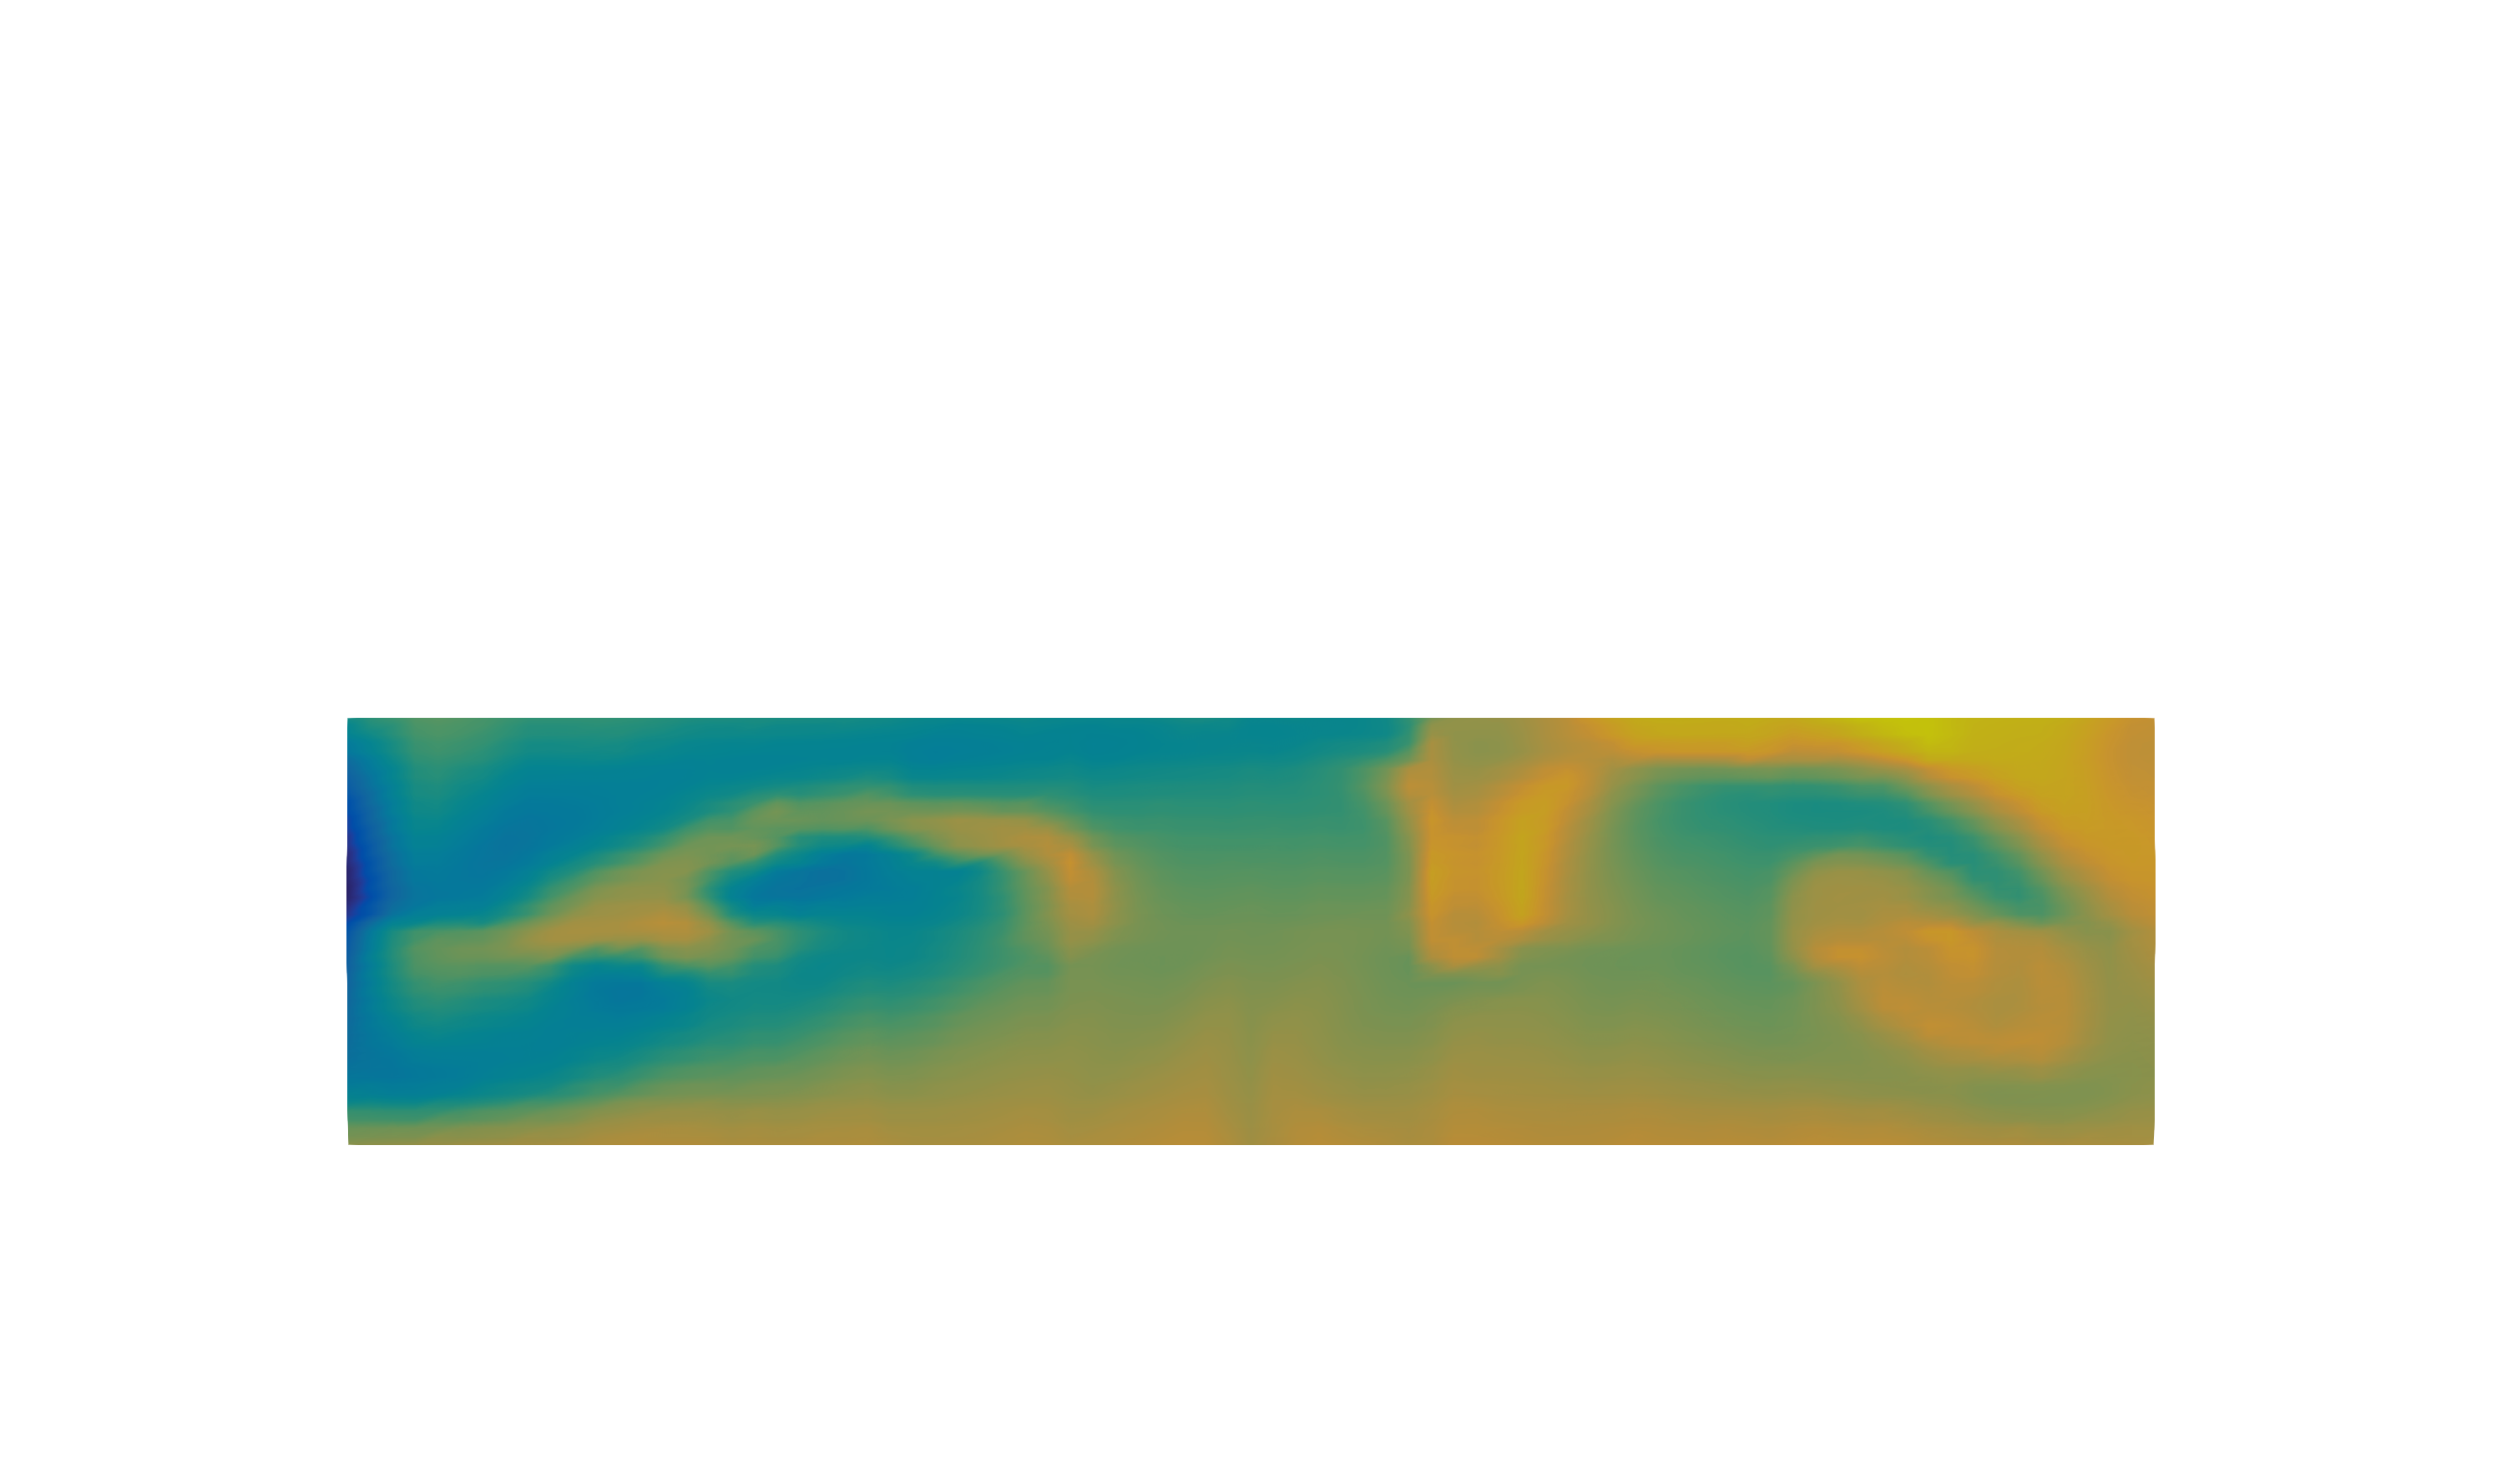
\includegraphics[width=\rasterimagewidth]{{../media/populations/application/print/alumina-influance-th1-2.54-3.08}.png}}};
        \end{axis}
      \end{tikzpicture}
      \begin{tikzpicture}
        \begin{axis}[
            %colorbar,
            hide axis,
            scale only axis,
            height=0.26\rasterimagewidth,,
            width=\rasterimagewidth,
            %colorbar horizontal,
            point meta min=2.54,
            point meta max=3.09,
            colorbar style={
              title=Concentration [\%w],
              width=7.4cm,
              height=0.3cm,
              xtick={2.54,2.75, 3,3.09, 3.5, 4, 4.5, 5, 5.5, 6},
              at={(0.5\rasterimagewidth,0.4cm)},
              anchor=north
            }
          ]
          \addplot [] coordinates {(0,0)};
          \node (myfirstpic) at (0,0) {\framebox{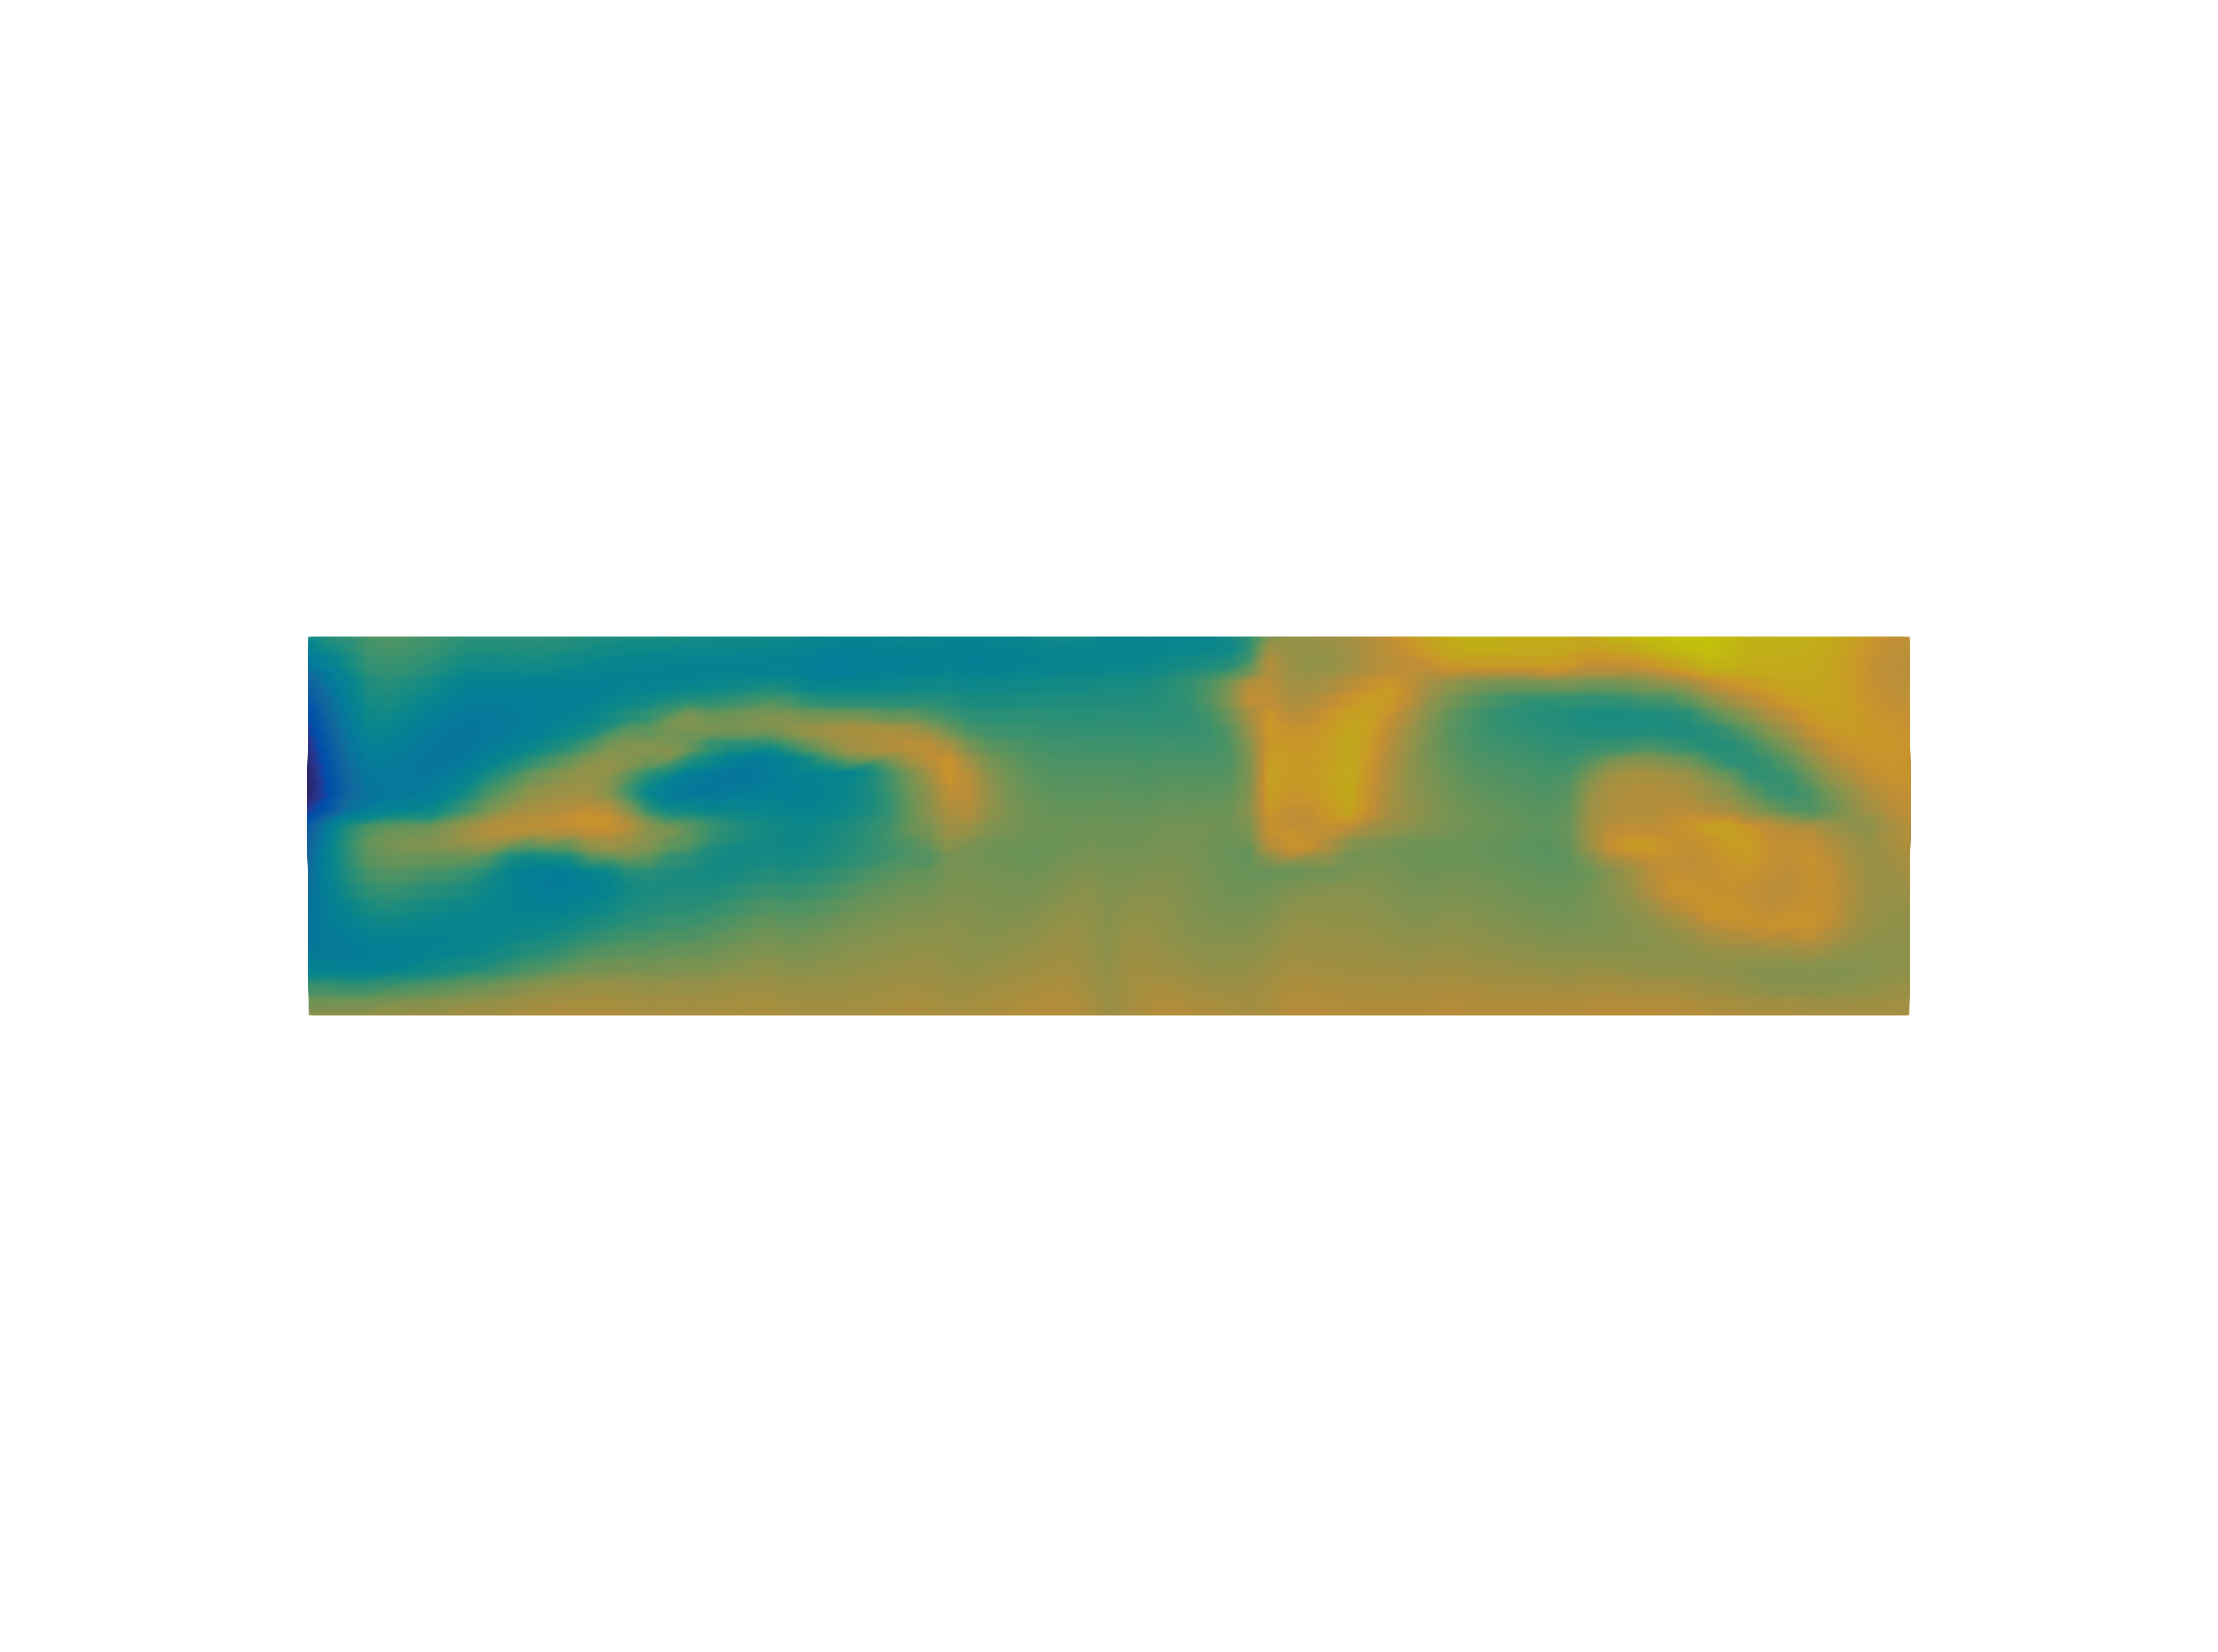
\includegraphics[width=\rasterimagewidth]{{../media/populations/application/print/alumina-influance-th2-2.54-3.09}.png}}};
        \end{axis}
      \end{tikzpicture}
      \begin{tikzpicture}
        \begin{axis}[
            %colorbar,
            hide axis,
            scale only axis,
            height=0.26\rasterimagewidth,,
            width=\rasterimagewidth,
            %colorbar horizontal,
            point meta min=2.54,
            point meta max=3.09,
            colorbar style={
              title=Concentration [\%w],
              width=7.4cm,
              height=0.3cm,
              xtick={2.54, 2.75, 3, 3.09, 3.5, 4, 4.5, 5, 5.5, 6},
              at={(0.5\rasterimagewidth,0.4cm)},
              anchor=north
            }
          ]
          \addplot [] coordinates {(0,0)};
          \node (myfirstpic) at (0,0) {\framebox{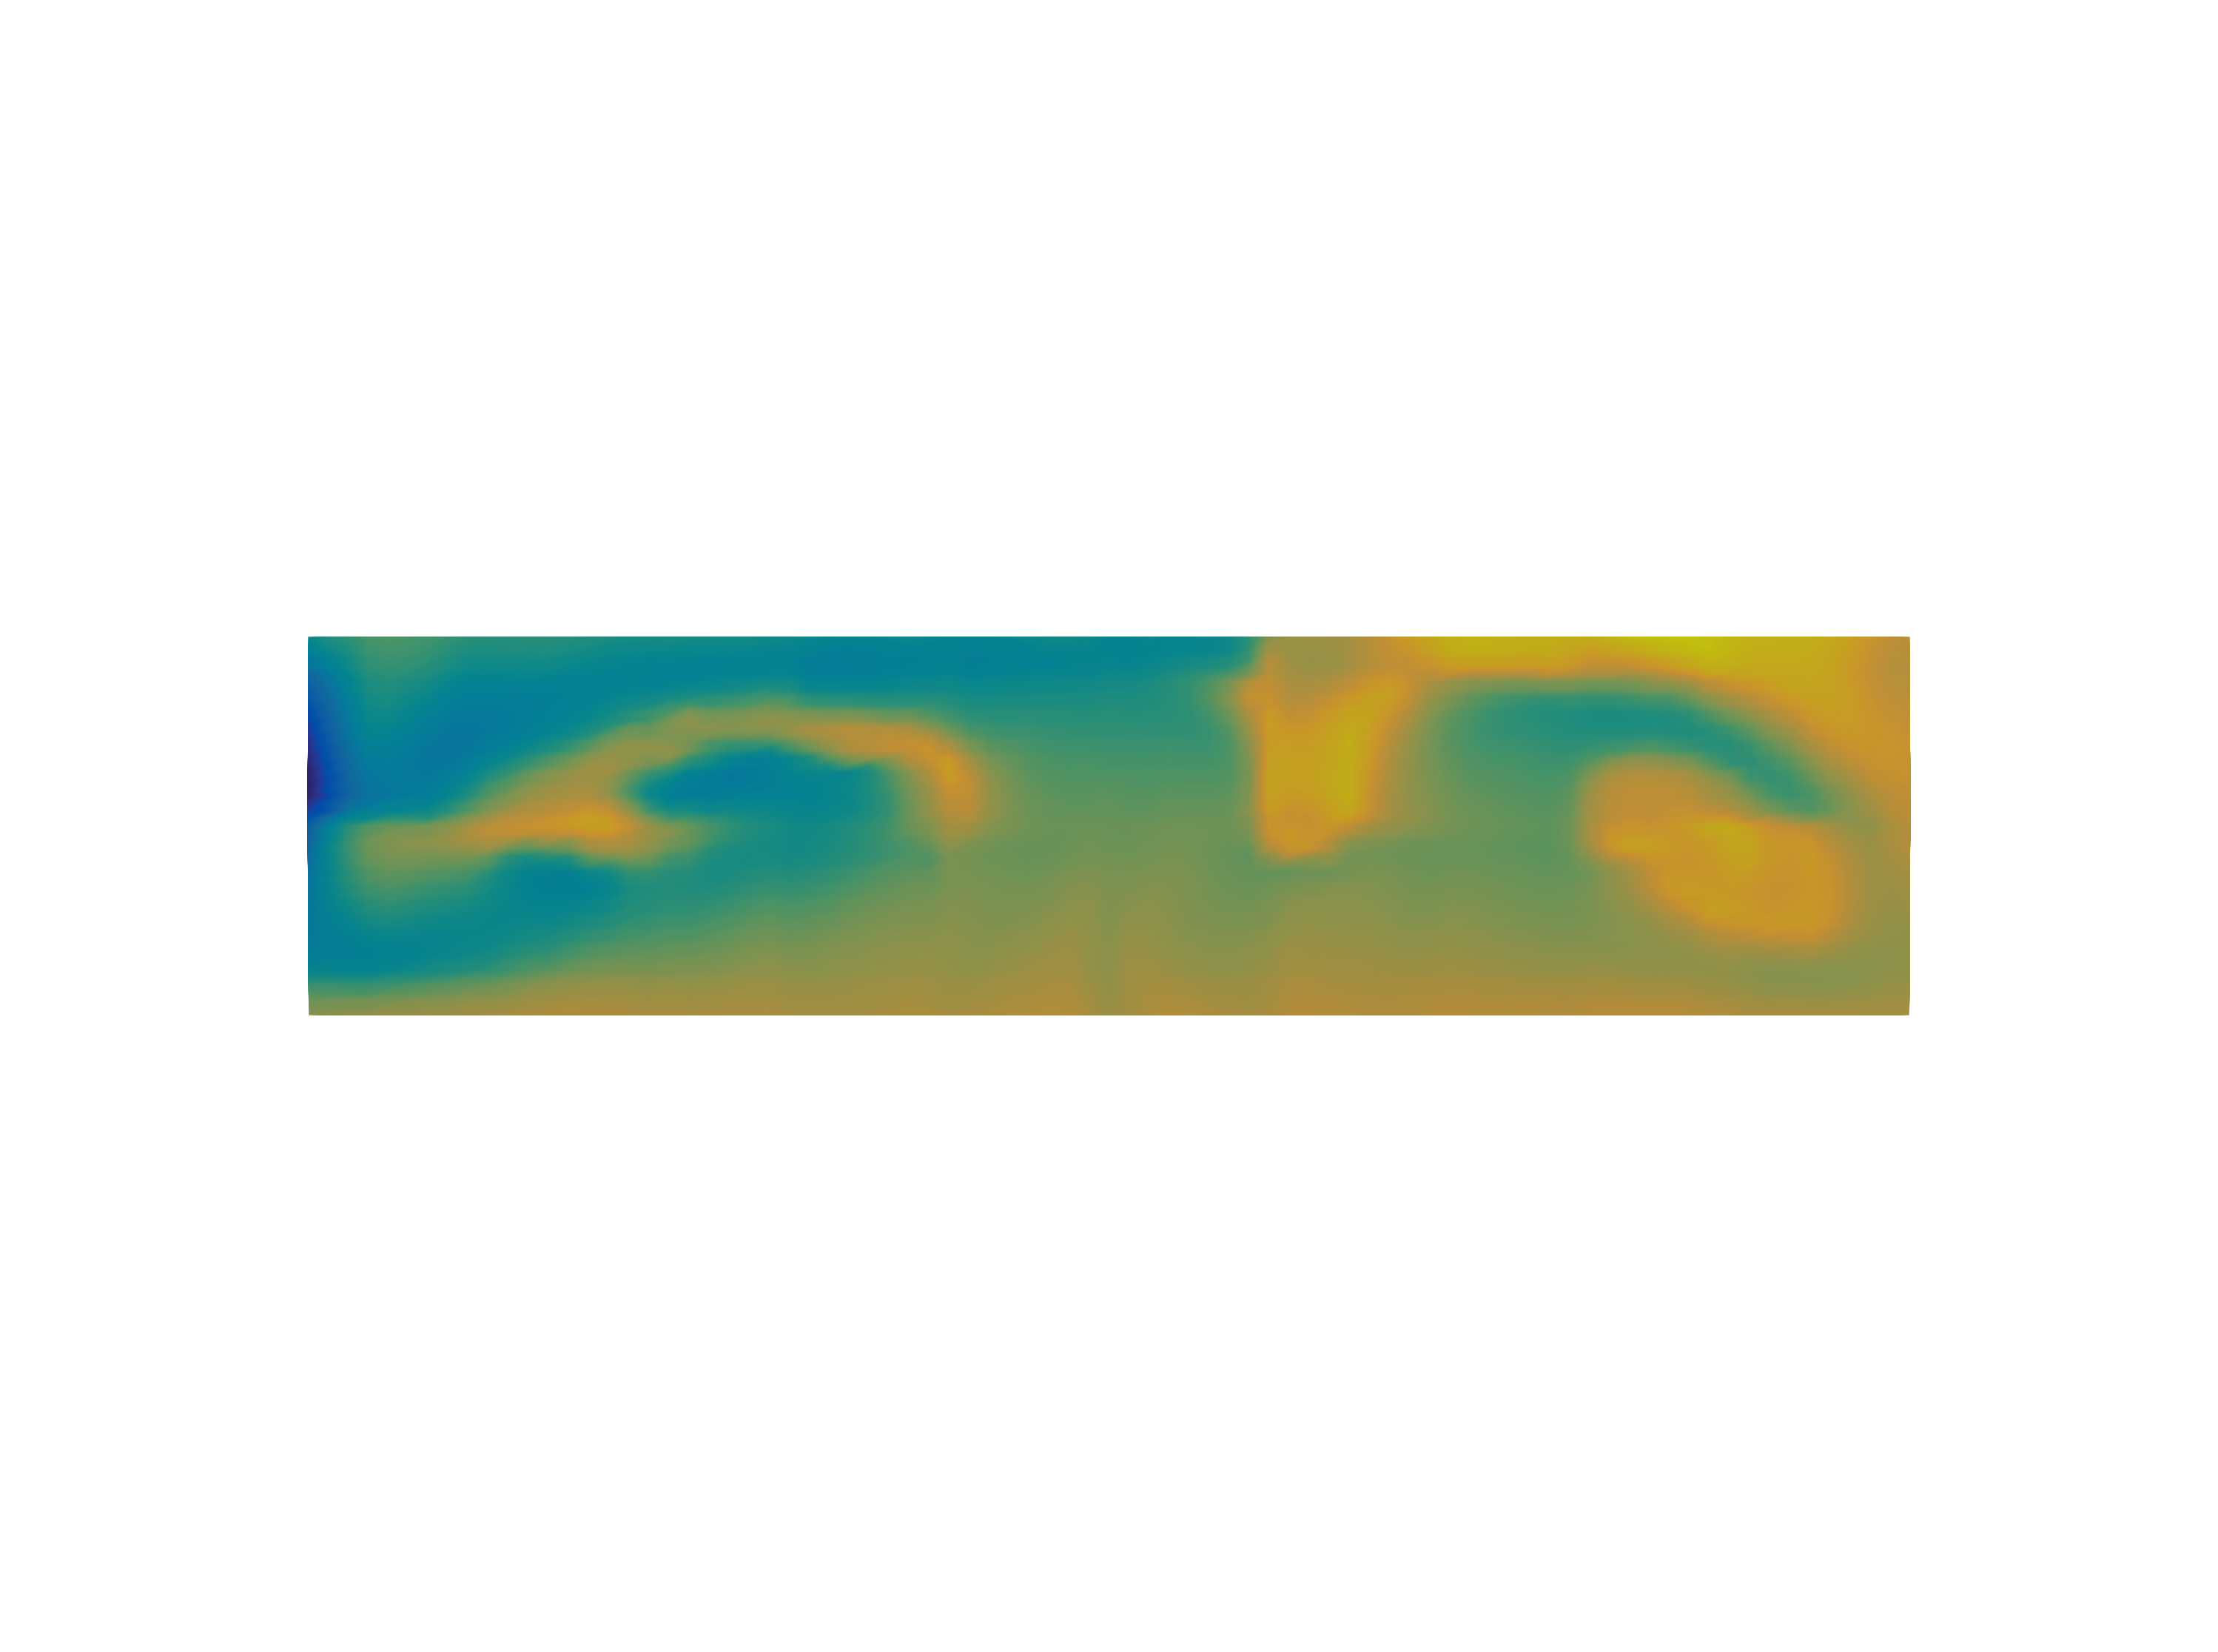
\includegraphics[width=\rasterimagewidth]{{../media/populations/application/print/alumina-influance-th5-2.54-3.09}.png}}};
        \end{axis}
      \end{tikzpicture}
      \begin{tikzpicture}
        \begin{axis}[
            colorbar,
            hide axis,
            scale only axis,
            height=0.52\rasterimagewidth,,
            width=\rasterimagewidth,
            colorbar horizontal,
            point meta min=2.54,
            point meta max=3.09,
            colorbar style={
              title=Concentration [\%w],
              width=7.4cm,
              height=0.3cm,
              xtick={2.54,2.75, 3, 3.09, 3.5, 4, 4.5, 5, 5.5, 6},
              at={(0.5\rasterimagewidth,3.0cm)},
              anchor=north
            }
          ]
          \addplot [] coordinates {(0,0)};
          \node (myfirstpic) at (0,50) {{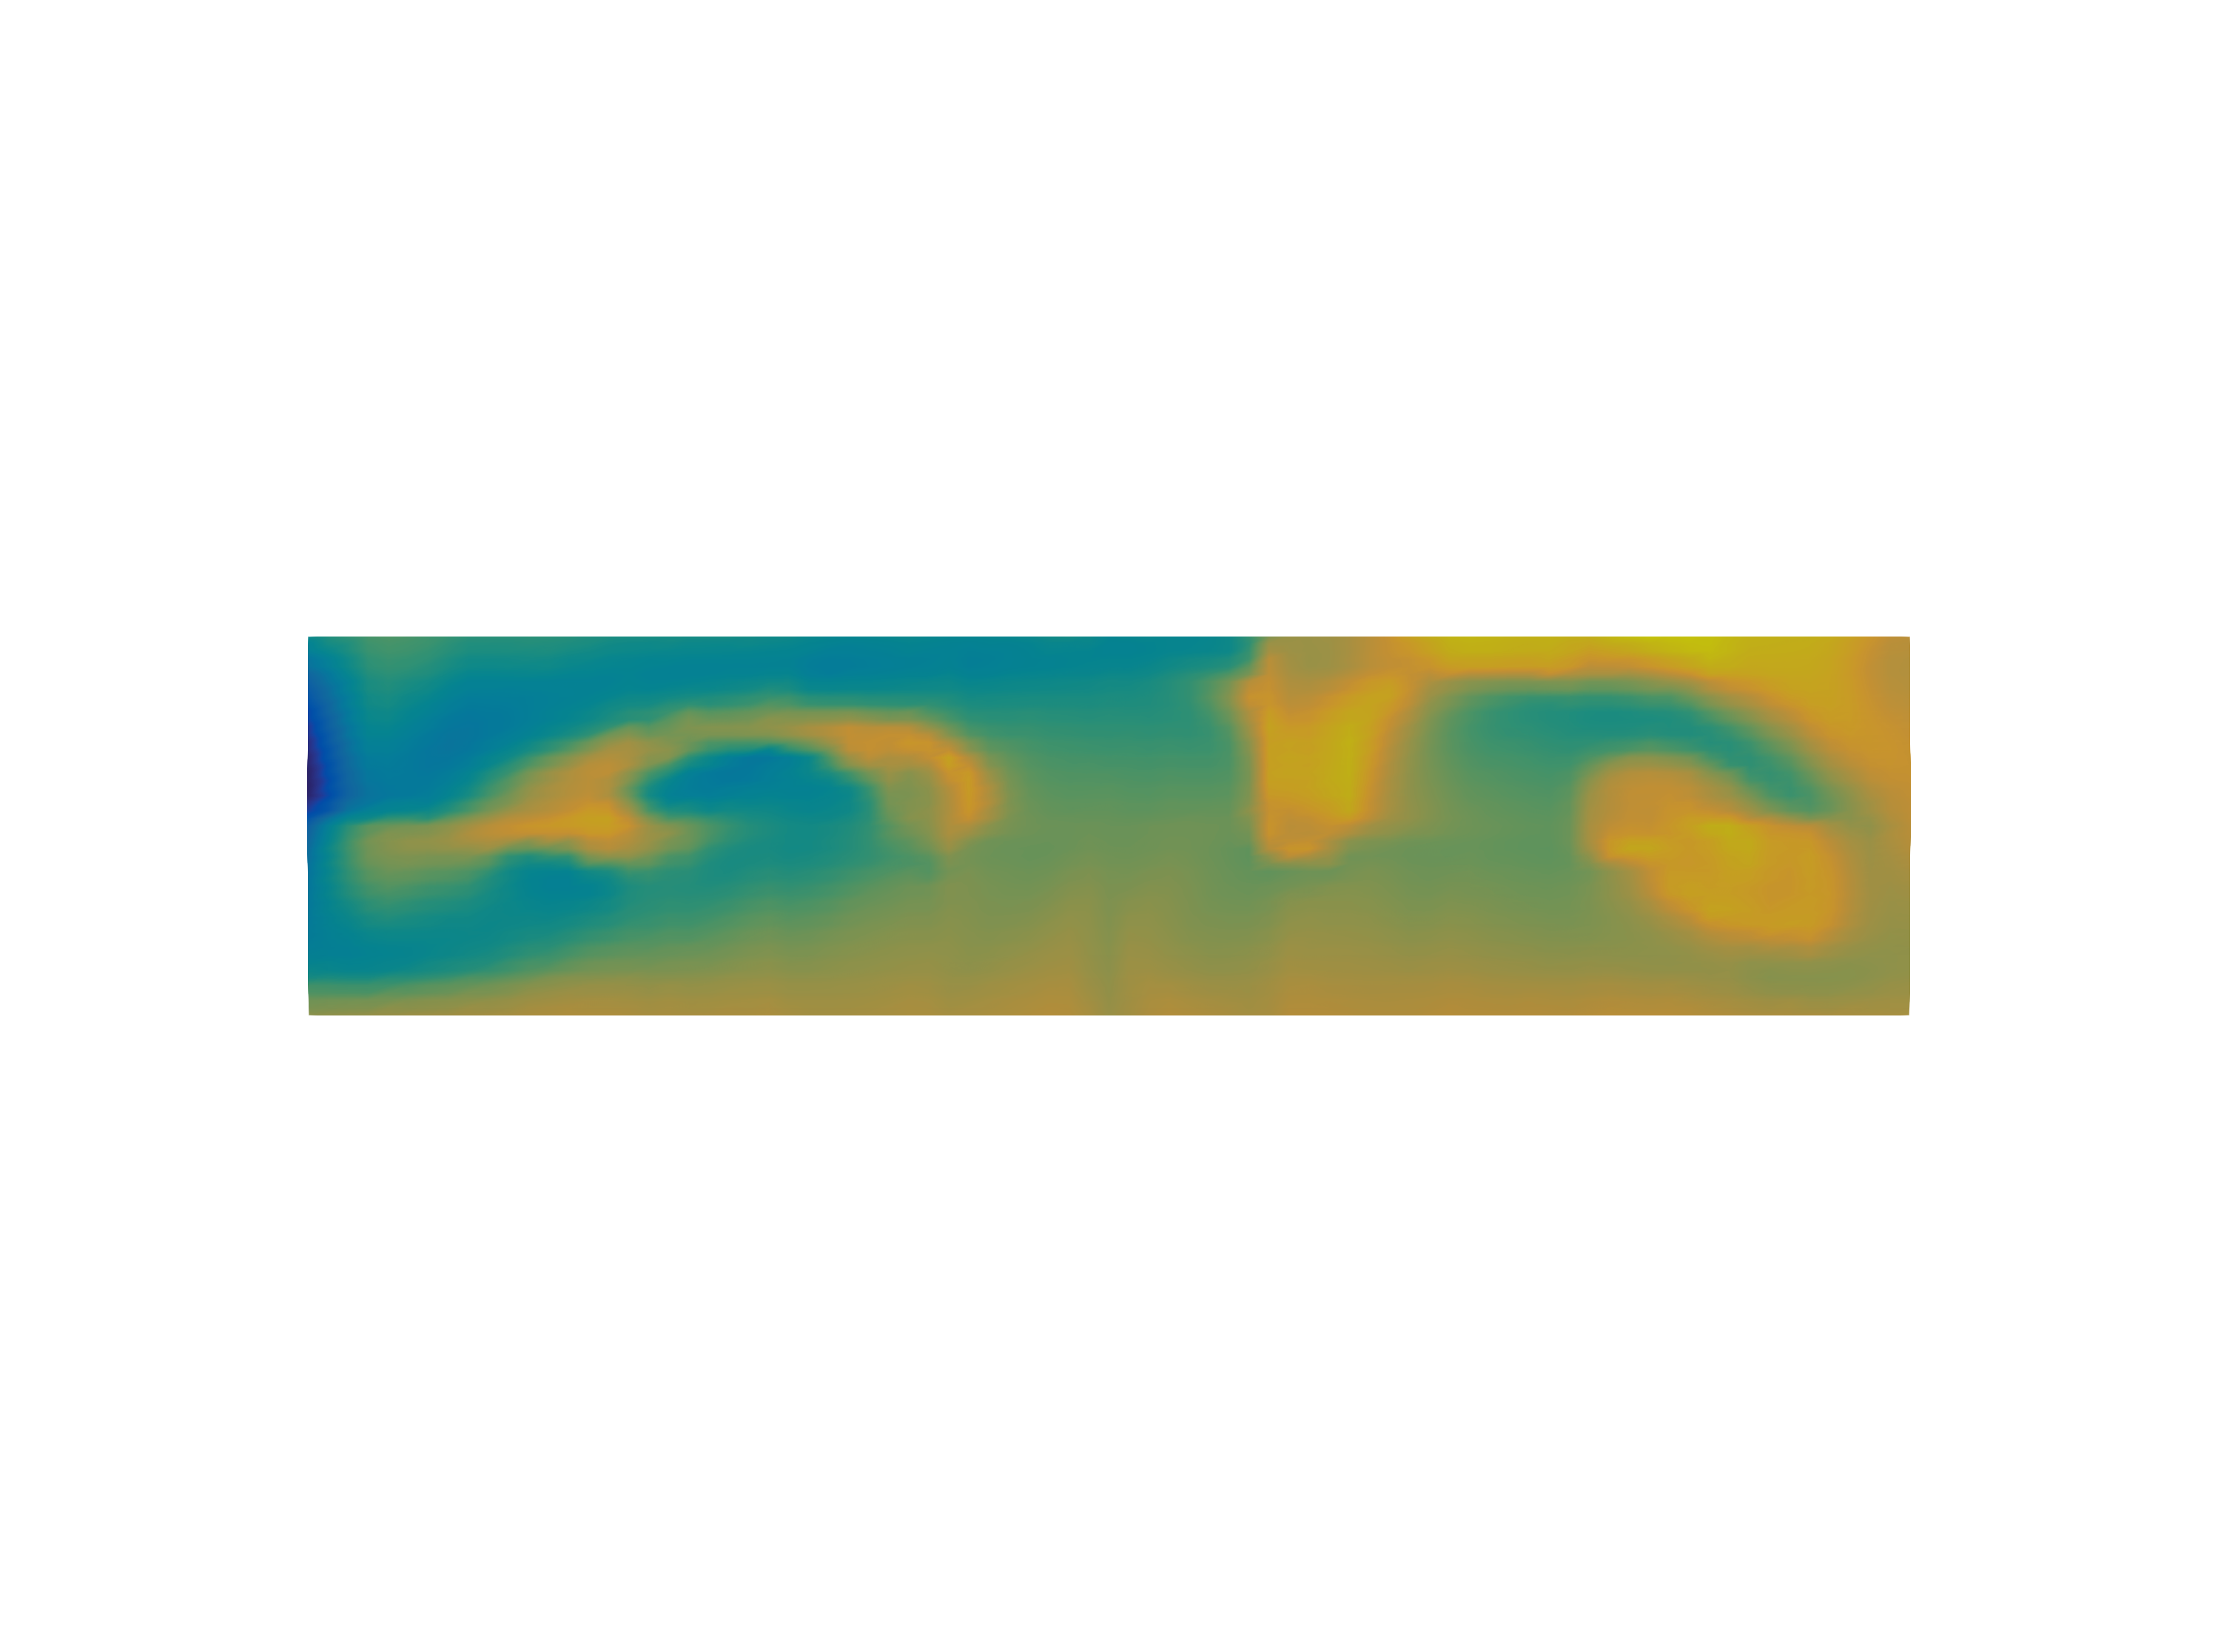
\includegraphics[width=\rasterimagewidth]{{../media/populations/application/print/alumina-influance-th510-2.54-3.09}.png}}};
        \end{axis}
      \end{tikzpicture}
    \caption{Champ de concentration $c$ dans l'ACD de la cuve AP32 à
      $t = \num{10000}$ \si{second}. De haut en bas, le temps de
      latence de dissolution $T_\text{Lat} = 1\si\second$,
      $2\si\second$, $5\si\second$ et $10\si\second$.}
    \label{fig:dissolution-alumin-influence-tlat}
  \end{center}
\end{figure}


La figure \ref{fig:dissolution-alumin-influence-tlat} présente la
distribution de concentration d'alumine dissoute dans l'ACD de la cuve
AP32 à $T = $ \num{10000} \si{\second} pour les différentes valeurs
de $\tlat$ croissantes de haut en bas.

Les quatre champs de concentration présentés sur la figure
\ref{fig:dissolution-alumin-influence-tlat} sont très similaires. Les
maximums et les minimum de la concentration d'alumine sont atteint
sont les mêmes et apparaissent aux mêmes endroits. On remarque
malgré tout de petites modification de la distribution d'alumine
dissoute au voisinage des points d'injection. On observe par exemple
autour du point d'injection \#2 que la concentration est plus diffuse
lorsque $\tlat$ croît.

Nous nous intéressons maintenant à l'effet de la température
initiale du bain sur la distribution de la concentration d'alumine dissoute.

% Sensibilité par rapport a la surchauffe du bain
\paragraph{Sensibilité par rapport à la surchauffe initiale du bain}
La vitesse de dissolution des particules dans l'électrolyte
(\ref{eq:dissolution-velocity}) dépend de la température locale de
celui-ci. Comme précisé plus haut dans cette section, sous
l'hypothèse que chaque dose de particules se dissout entièrement
en un temps fini, le terme source d'énergie par effet Joule est
construit de sorte à maintenir une quantité d'énergie thermique
constante en moyenne dans le temps. En l'absence de transition de
phase dans l'électrolyte, cela signifie que la température moyenne au
cours du temps de celui-ci est maintenue constante. Par conséquent,
une température initiale du bain $\tinit$ plus élevée résulte en une
température $\temperature$ dans l'état stationnaire périodique plus
élevée en moyenne au cours d'une période du cycle d'injection global.

\begin{figure}[!hp]
  \begin{center}
      \begin{tikzpicture}
        \begin{axis}[
            %colorbar,
            hide axis,
            scale only axis,
            height=0.41\rasterimagewidth,,
            width=\rasterimagewidth,
            %colorbar horizontal,
            point meta min=2.43,
            point meta max=3.05,
            colorbar style={
              title=Concentration [\%w],
              width=7.4cm,
              height=0.3cm,
              xtick={2.43,2.5,2.75, 3, 3.05, 3.5, 4, 4.5, 5, 5.5, 6},
              at={(0.5\rasterimagewidth,0.4cm)},
              anchor=north
            }
          ]
          \addplot [] coordinates {(0,0)};
          \node (myfirstpic) at (0,0) {\framebox{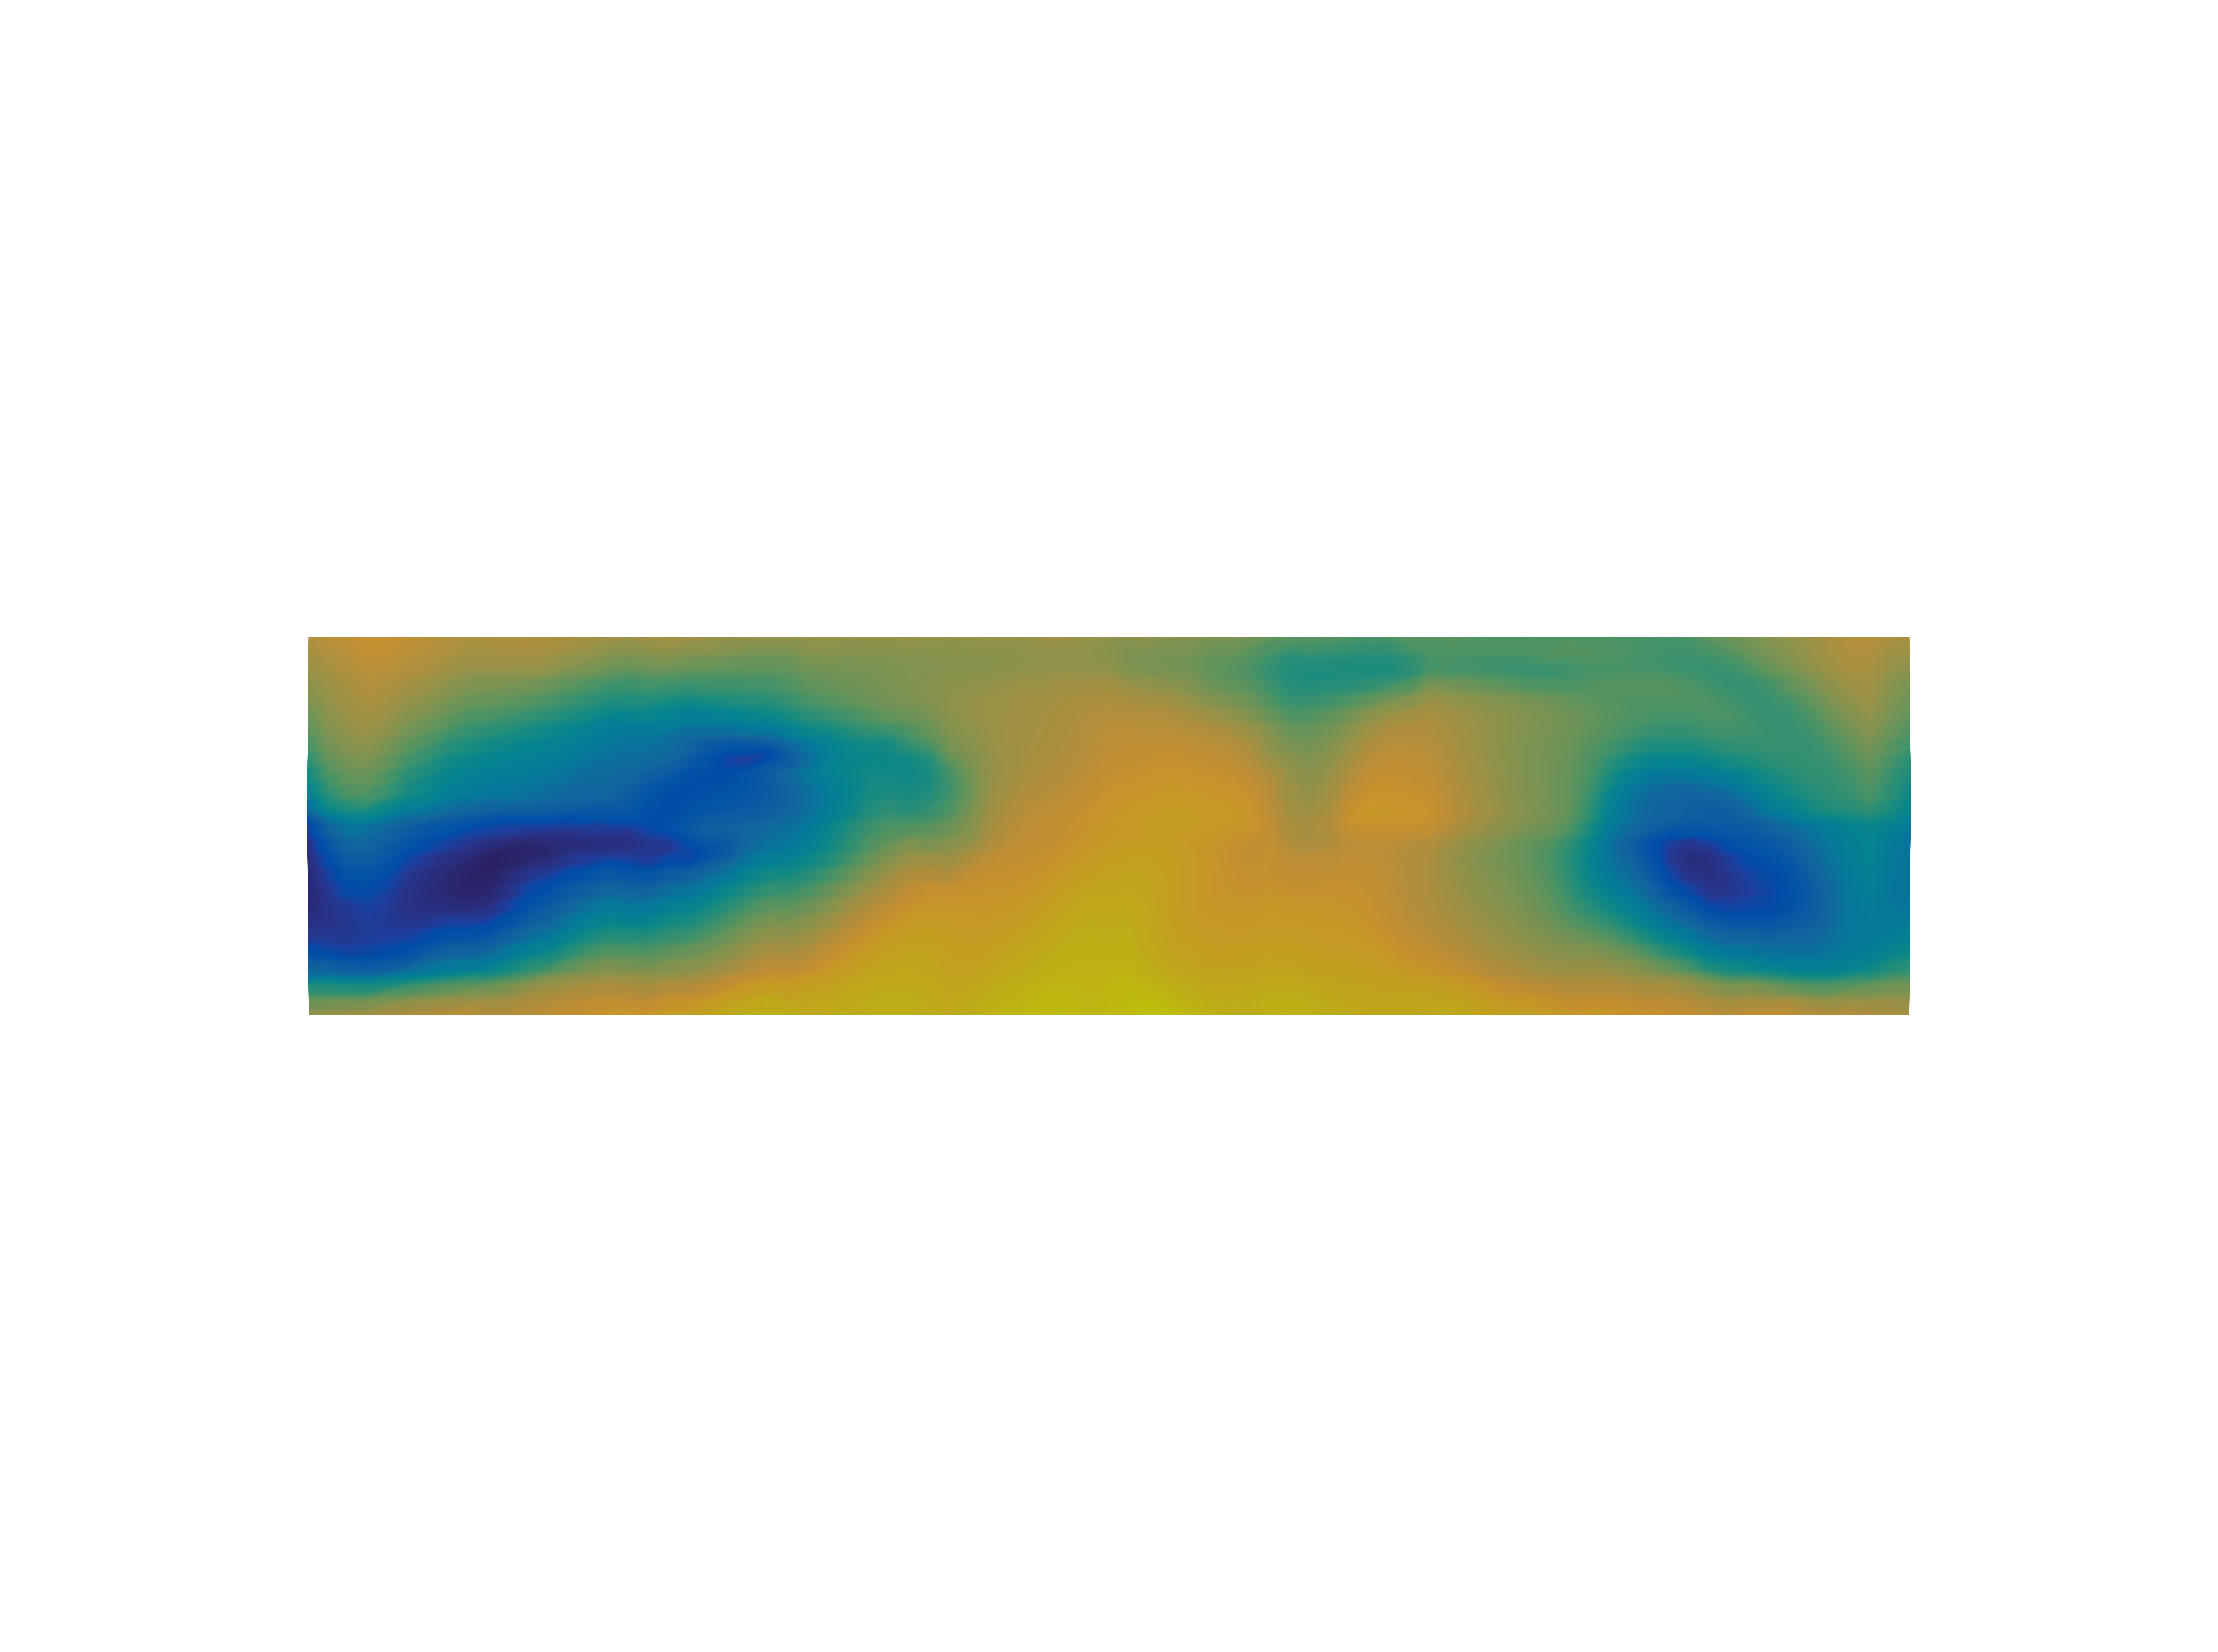
\includegraphics[width=\rasterimagewidth]{{../media/populations/application/print/alumina-influance-sur1-2.43-3.05}.png}}};
        \end{axis}
      \end{tikzpicture}
      \begin{tikzpicture}
        \begin{axis}[
            %colorbar,
            hide axis,
            scale only axis,
            height=0.41\rasterimagewidth,,
            width=\rasterimagewidth,
            %colorbar horizontal,
            point meta min=2.51,
            point meta max=3.02,
            colorbar style={
              title=Concentration [\%w],
              width=7.4cm,
              height=0.3cm,
              xtick={2.51,2.75, 3,3.02, 3.5, 4, 4.5, 5, 5.5, 6},
              at={(0.5\rasterimagewidth,0.4cm)},
              anchor=north
            }
          ]
          \addplot [] coordinates {(0,0)};
          \node (myfirstpic) at (0,0) {\framebox{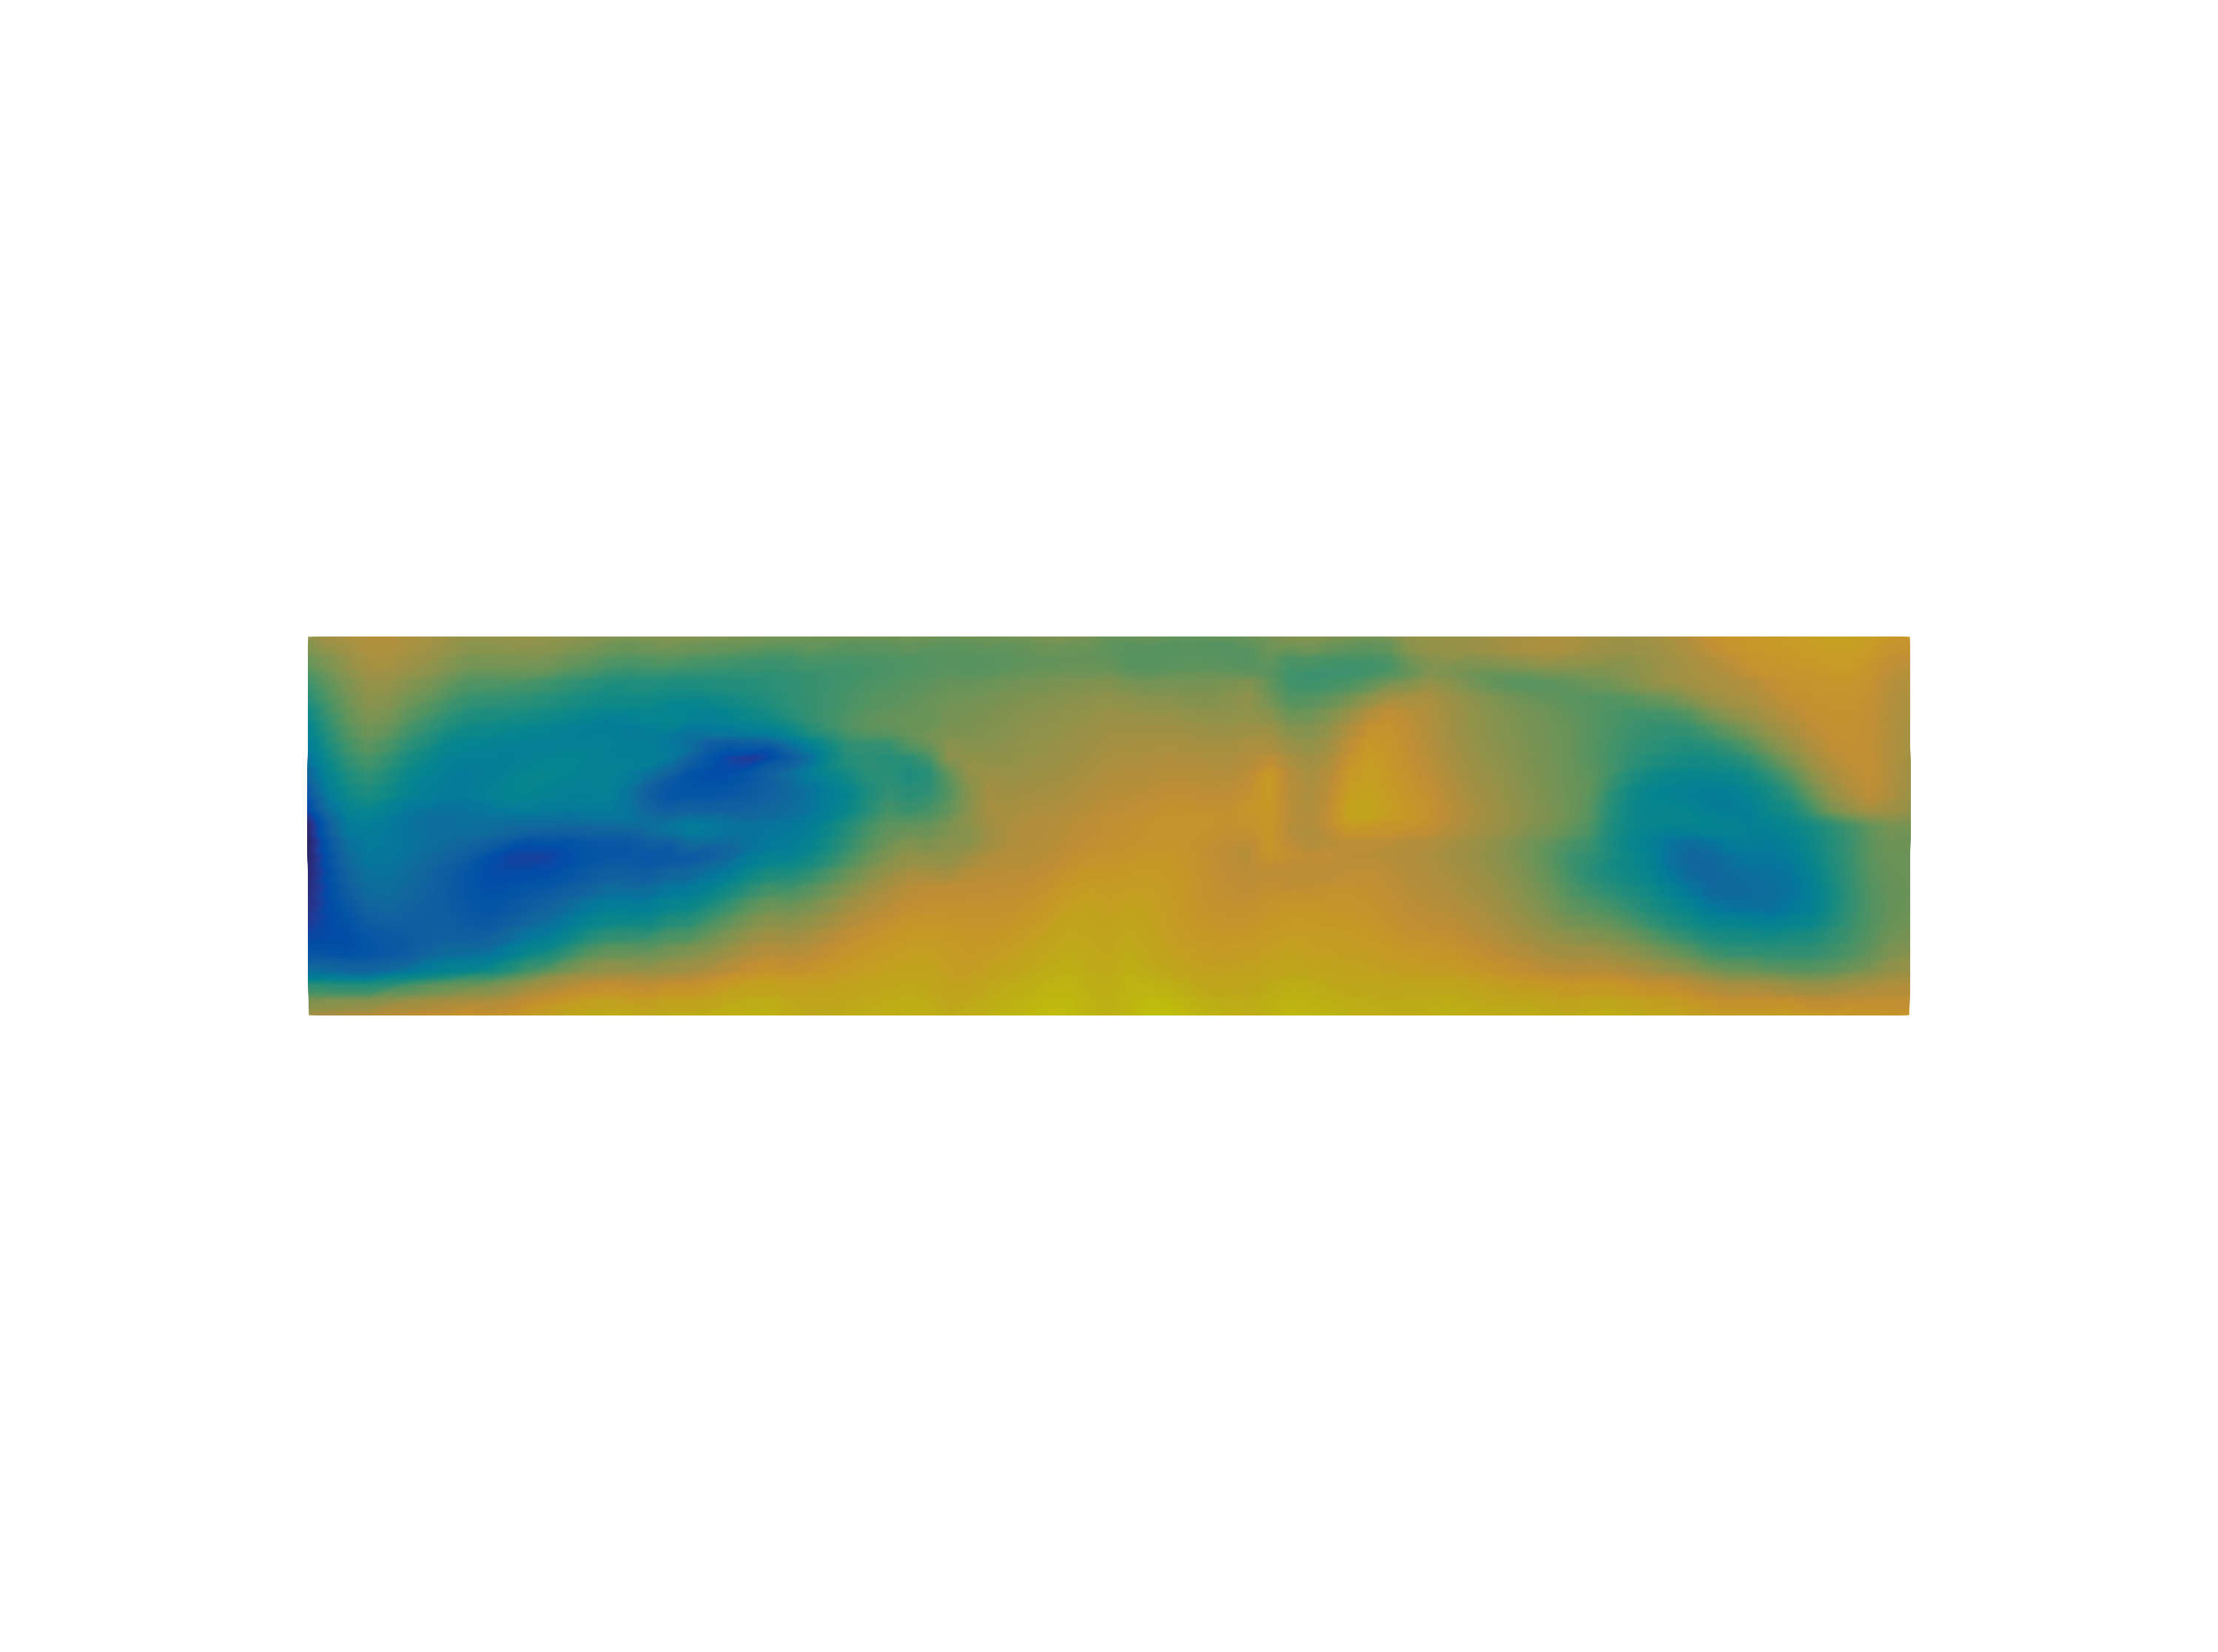
\includegraphics[width=\rasterimagewidth]{{../media/populations/application/print/alumina-influance-sur2-2.51-3.02}.png}}};
        \end{axis}
      \end{tikzpicture}
      \begin{tikzpicture}
        \begin{axis}[
            %colorbar,
            hide axis,
            scale only axis,
            height=0.41\rasterimagewidth,,
            width=\rasterimagewidth,
            %colorbar horizontal,
            point meta min=2.51,
            point meta max=3.13,
            colorbar style={
              title=Concentration [\%w],
              width=7.4cm,
              height=0.3cm,
              xtick={2.51,2.75, 3,3.13, 3.5, 4, 4.5, 5, 5.5, 6},
              at={(0.5\rasterimagewidth,0.4cm)},
              anchor=north
            }
          ]
          \addplot [] coordinates {(0,0)};
          \node (myfirstpic) at (0,0) {\framebox{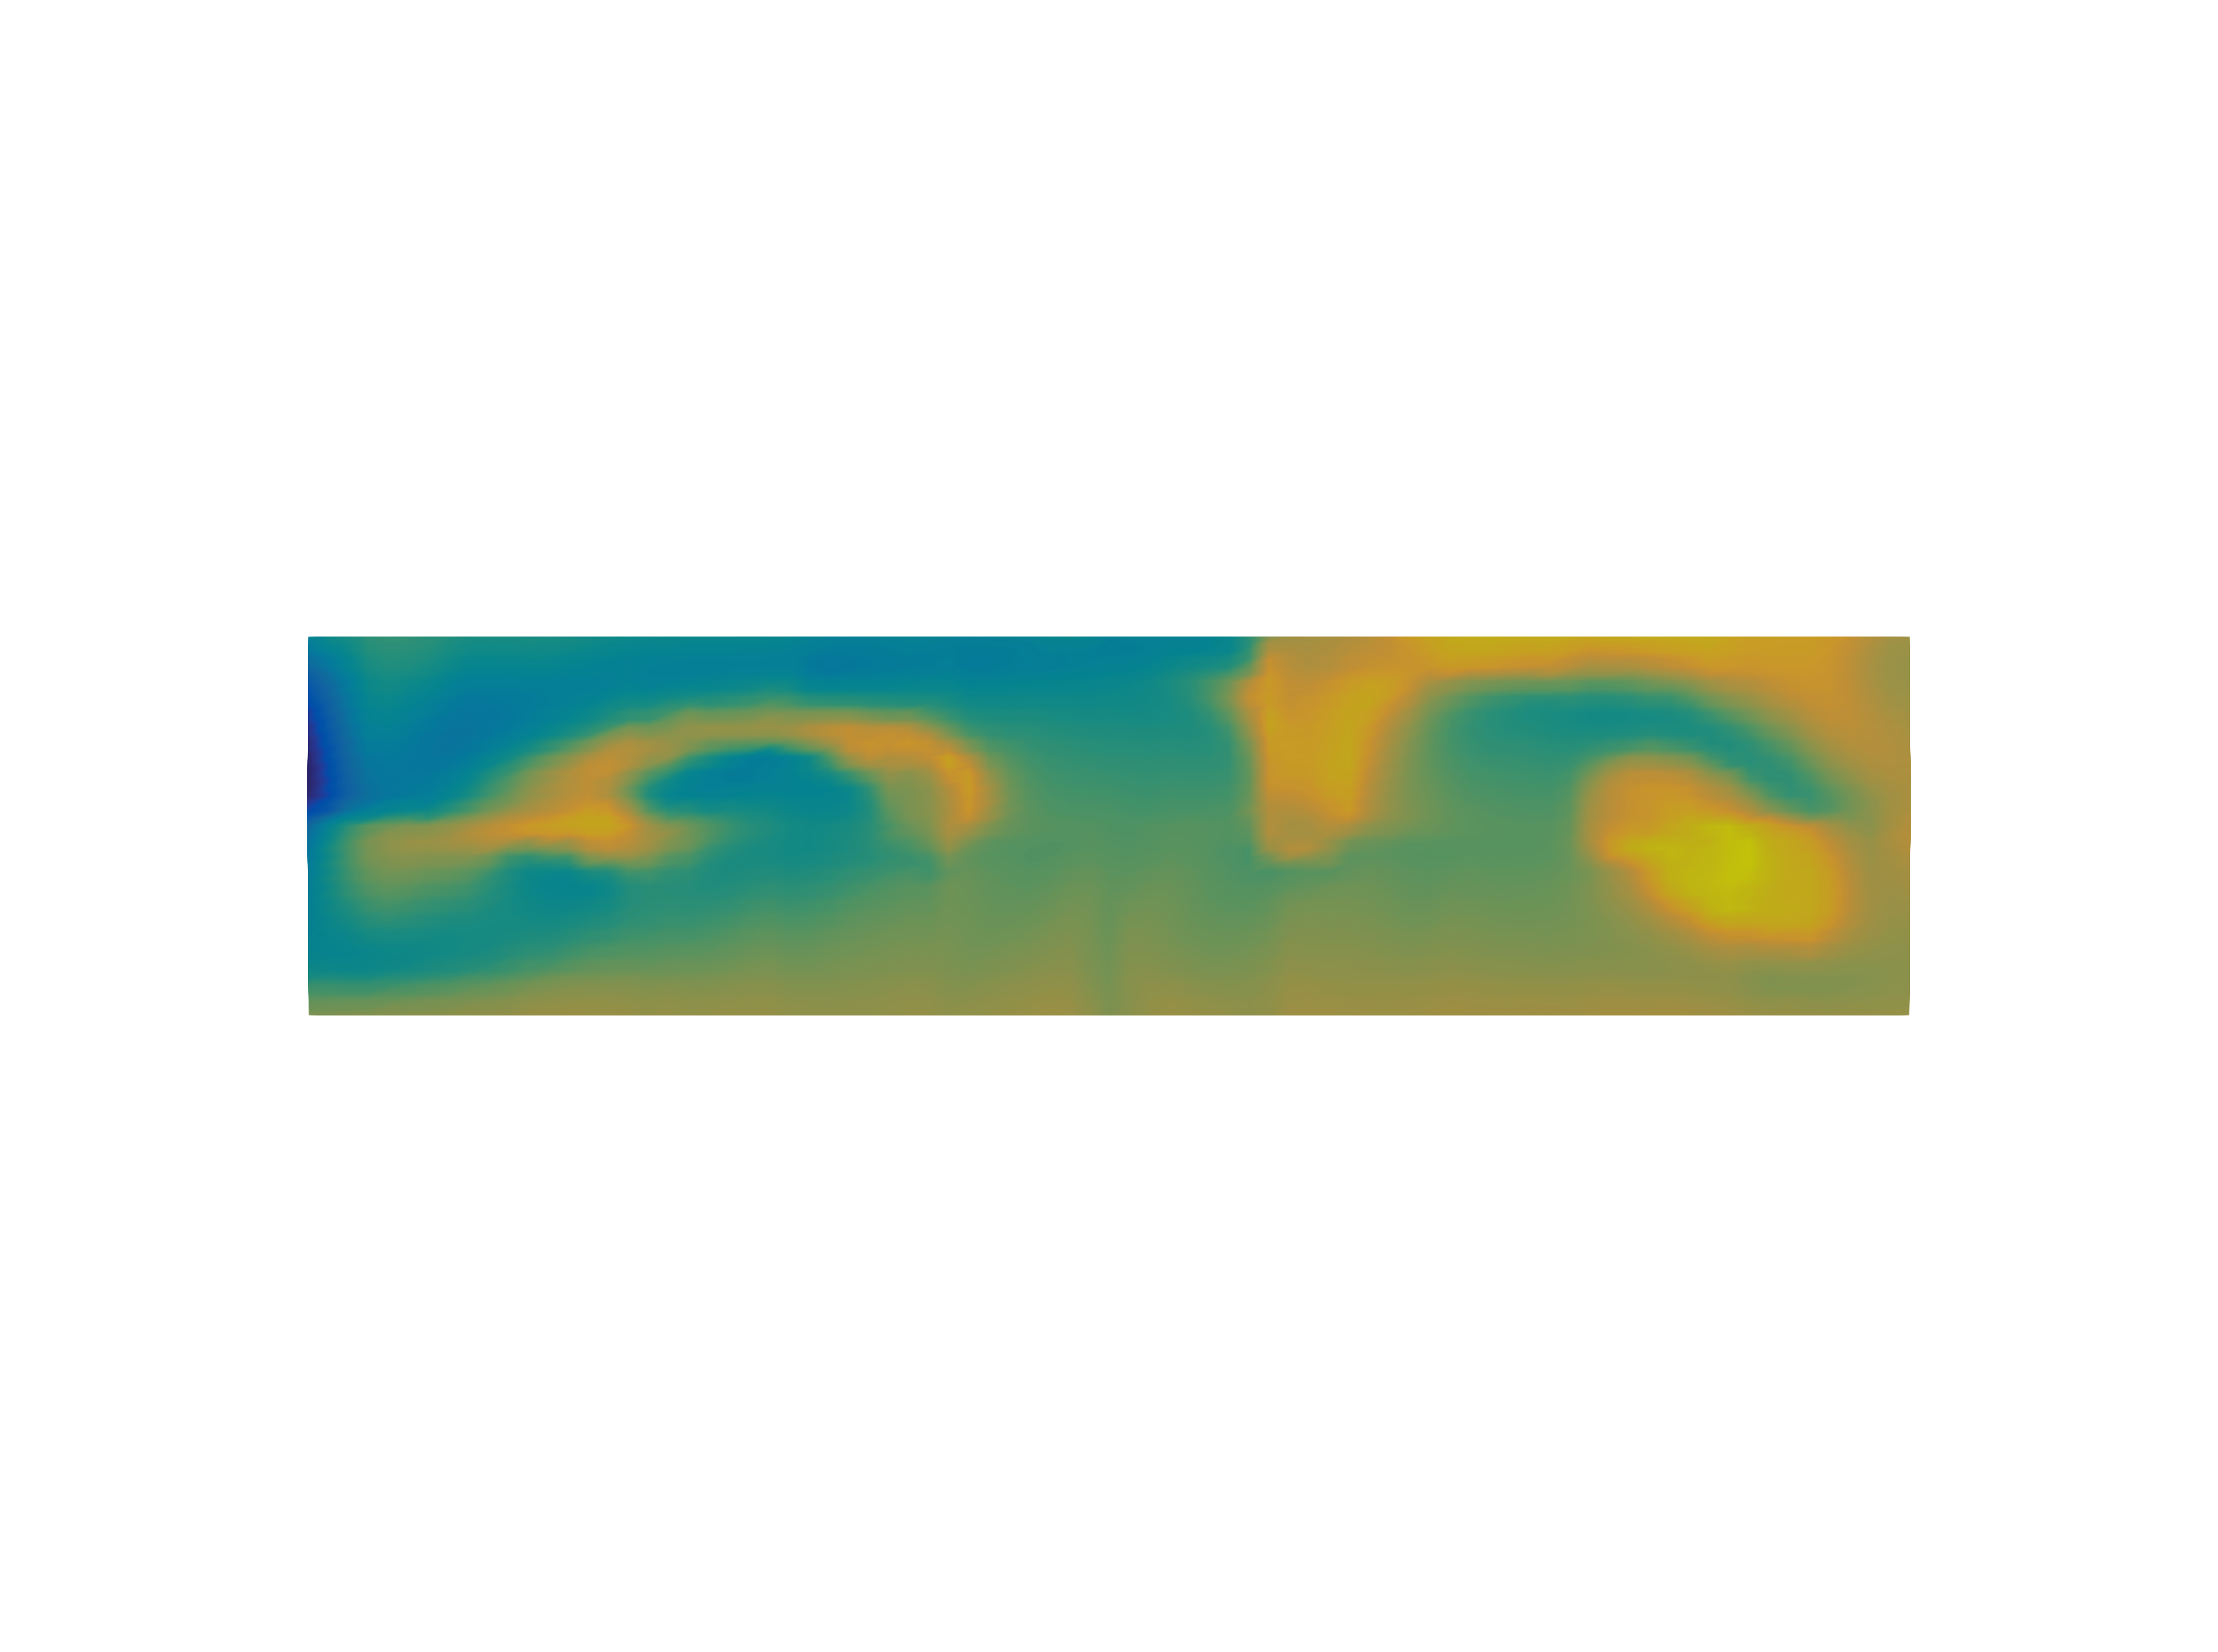
\includegraphics[width=\rasterimagewidth]{{../media/populations/application/print/alumina-influance-sur5-2.51-3.13}.png}}};
        \end{axis}
      \end{tikzpicture}
      \begin{tikzpicture}
        \begin{axis}[
            colorbar,
            hide axis,
            scale only axis,
            height=0.41\rasterimagewidth,,
            width=\rasterimagewidth,
            colorbar horizontal,
            point meta min=2.51,
            point meta max=3.13,
            colorbar style={
              title=Concentration [\%w],
              width=7.4cm,
              height=0.3cm,
              xtick={2.51, 2.75, 3, 3.13, 3.5, 4, 4.5, 5, 5.5, 6},
              at={(0.5\rasterimagewidth,0.4cm)},
              anchor=north
            }
          ]
          \addplot [] coordinates {(0,0)};
          \node (myfirstpic) at (0,0) {\framebox{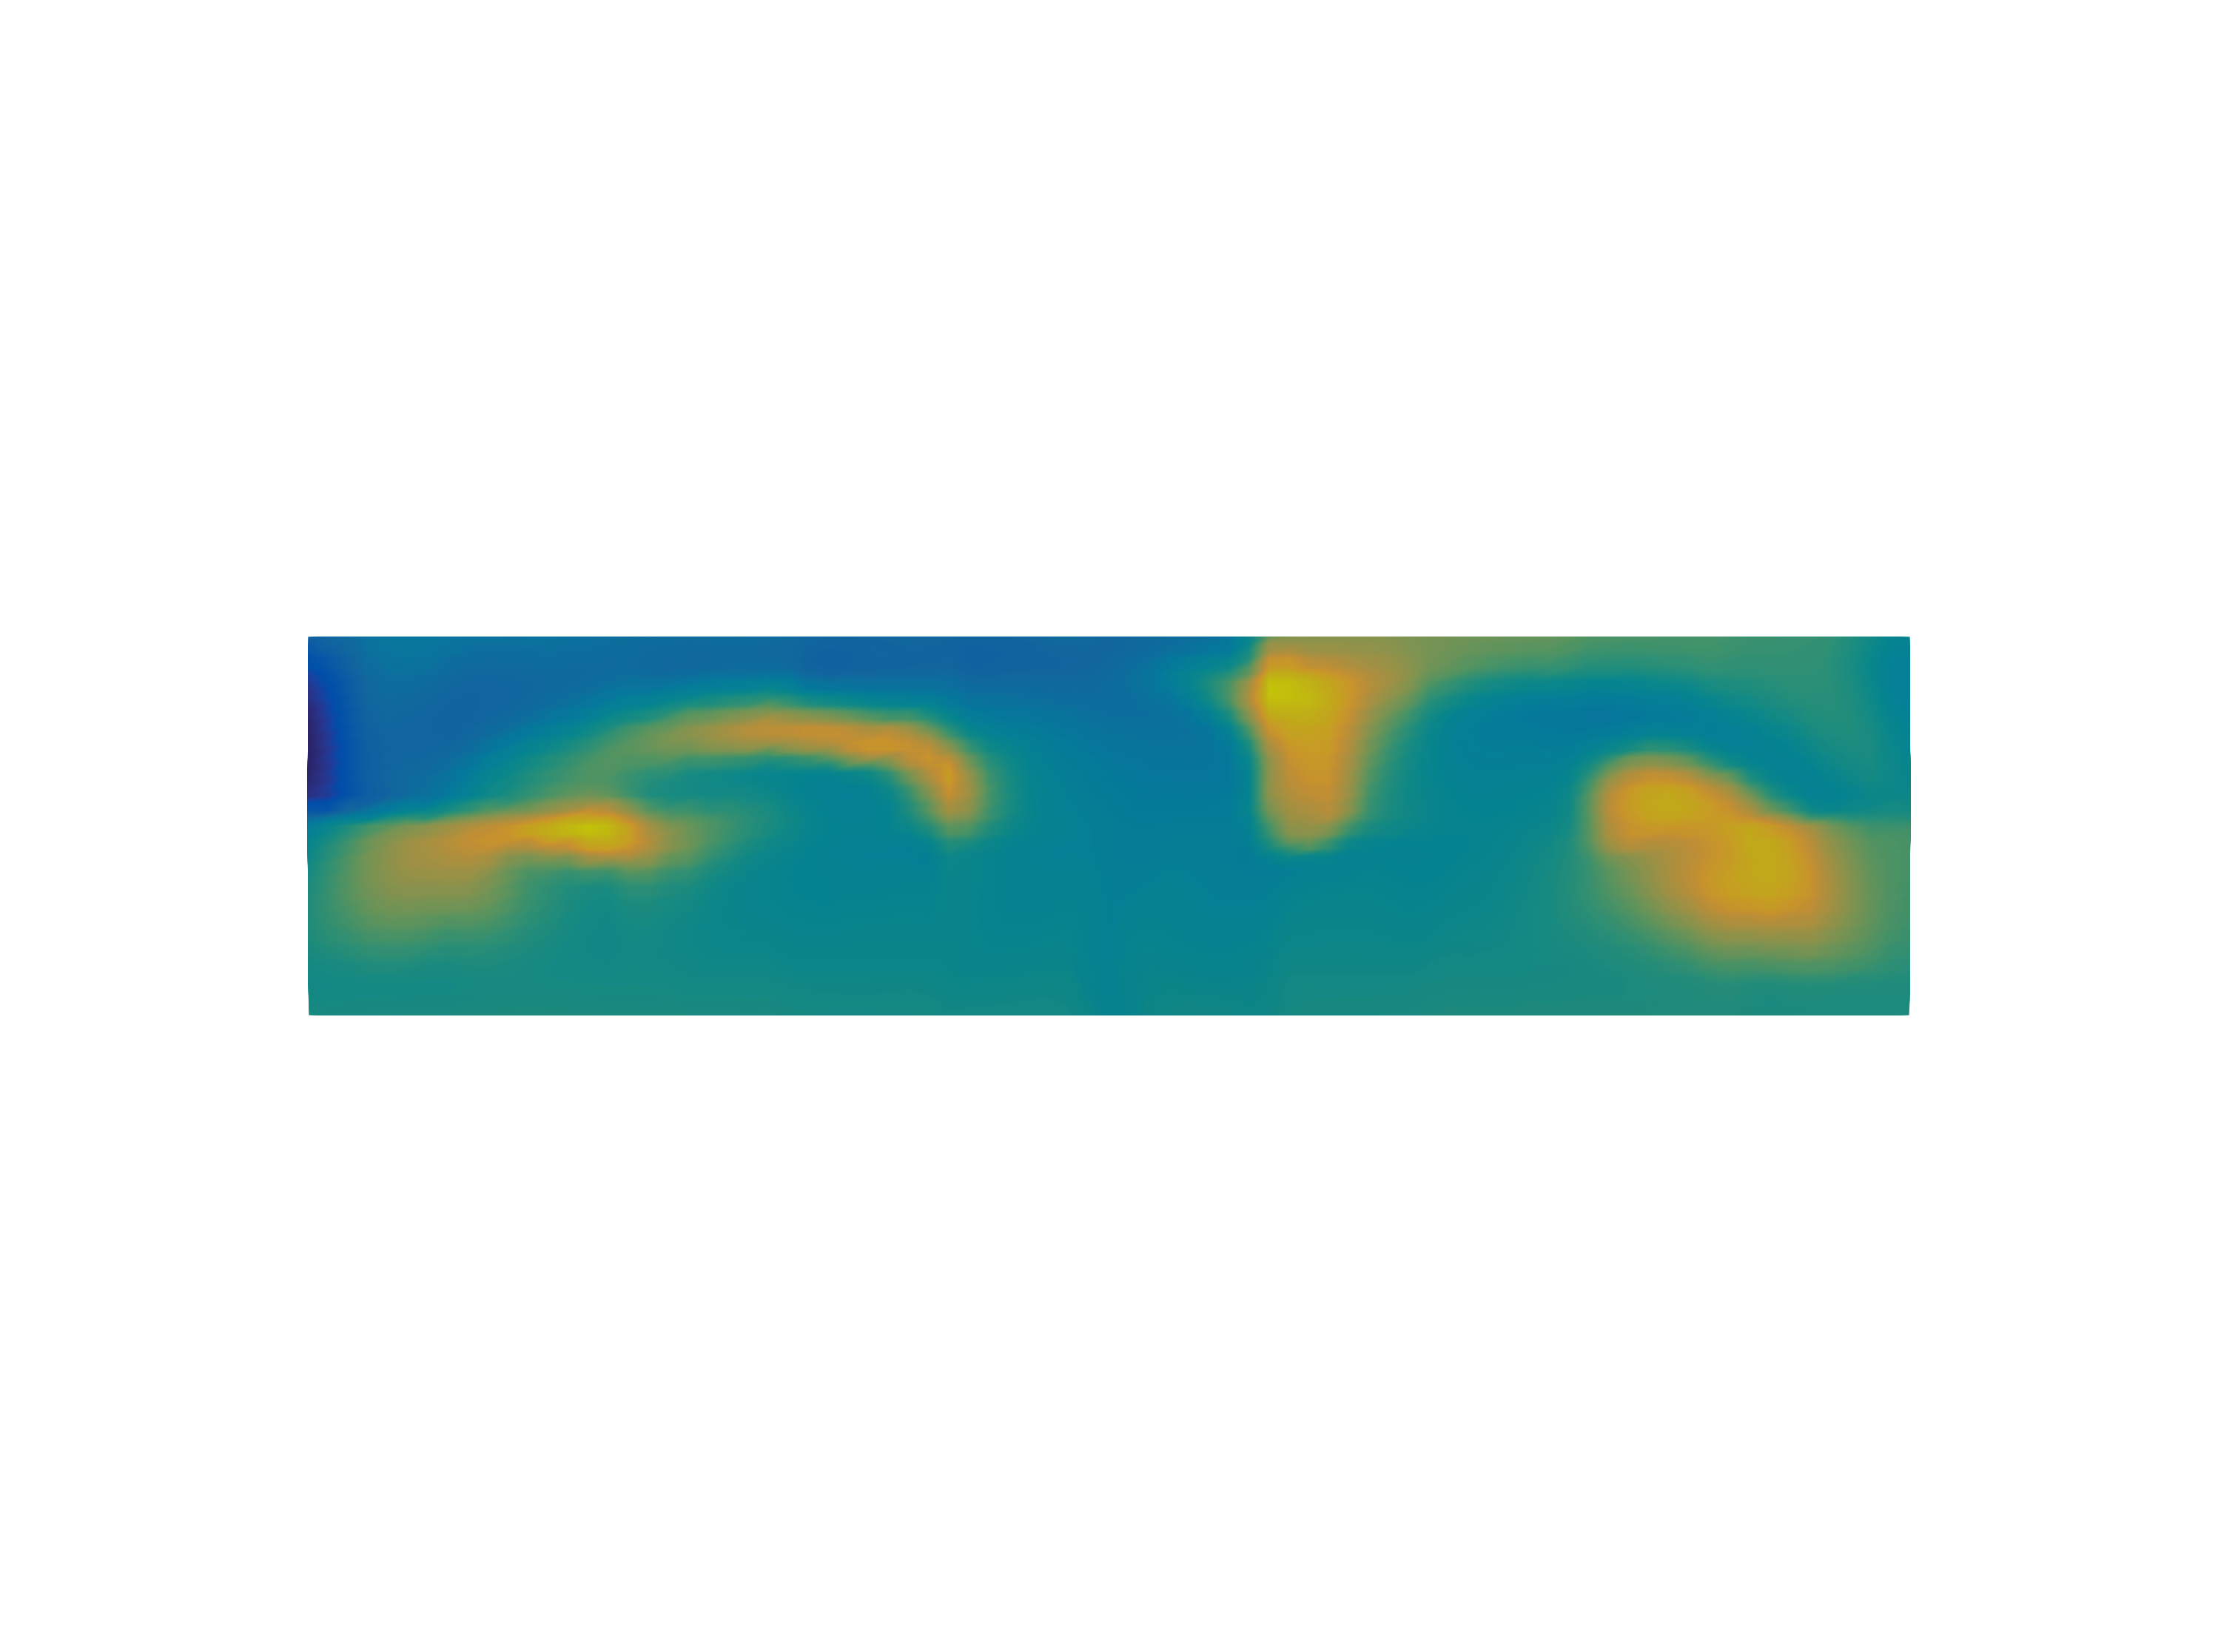
\includegraphics[width=\rasterimagewidth]{{../media/populations/application/print/alumina-influance-sur10-2.51-3.13}.png}}};
        \end{axis}
      \end{tikzpicture}
      \caption{Champ de concentration $c$ dans l'ACD de la cuve AP32 à
        $t = \num{10000}$ \si{\second}. De haut en bas, la température
        de surchauffe initiale est $\tsur = $ \numlist{1;2;5;10}.}
    \label{fig:dissolution-alumin-influence-sur}
  \end{center}
\end{figure}


Nous proposons d'évaluer la sensibilité de la dissolution d'alumine
dans le bain électrolytique en fonction de la température de celui-ci
en faisant varier la température initiale du bain. On note $\tsur$ la
température de surchauffe initiale du bain au-dessus de sa température de
liquidus:
\begin{equation}
  \tsur = \tinit - \tliq.
\end{equation}
La figure \ref{fig:dissolution-alumin-influence-sur} présente la distribution
de la concentration d'alumine dissoute $c$ dans l'ACD de la cuve AP32
issue de quatre calculs, pour lesquels les paramètres sont reportés
dans la table \ref{tab:dissolution-physical-parameters}, à
l'exception de la température initiale du bain $\tinit$. La
température initiale du bain est fixée à $\tinit = \tliq + \tsur$ avec $\tsur = $ \numlist{1;2;5;10} kelvin.

Les champs de concentration sur la figure
\ref{fig:dissolution-alumin-influence-sur} correspondent de haut en
bas à des température de surchauffe $\tsur$ croissante. On remarque
en particulier sur le dernier champ de concentration de cette figure,
qui correspond à $\tsur = $ \num{10} \si{\kelvin}, la similarité avec la
solution de référence illustrée sur la figure
\ref{fig:ap32-alumina-wo-t} pour laquelle la température ne joue pas
de rôle dans la dissolution des particules. Les valeurs maximales
atteinte par la concentration d'alumine dissoute sont cependant plus faibles.

Le premier champ de concentration de la figure
\ref{fig:dissolution-alumin-influence-sur} correspond à une
température de surchauffe $\tsur =$ \num{1} \si{\kelvin} et s'écarte
significativement de la solution de référence. La concentration
d'alumine dissoute est homogène au point de ne plus pouvoir
distinguer la position des injecteurs.

La dissolution des particules d'alumine dépend d'une part du fait que
la température de l'électrolyte dans leur voisinage doit être
supérieure à la température du liquidus $\tliq$, et d'autre part de la
taille de la région de transition entre le régime de dissolution
contrôlé par la diffusion de l'énergie thermique et le régime de
dissolution contrôlé par la diffusion de l'alumine dissoute à
proximité de la surface des particules. La transition entre ces deux
régimes est contrôlée par le paramètre $\tcrit$. Dans le paragraphe
suivant nous proposons d'évaluer la distribution de concentration dans
le bain électrolytique en fonction du paramètre $\tcrit$.


\clearpage
% Sensibilité par rapport au modèle de dépendence (tcrit, exp vs heaviside)
\paragraph{Sensibilité par rapport à la température critique de transition}
\begin{figure}[!hp]
  \begin{center}
      \begin{tikzpicture}
        \begin{axis}[
            colorbar,
            hide axis,
            scale only axis,
            height=0.41\rasterimagewidth,
            width=\rasterimagewidth,
            colorbar horizontal,
            point meta min=2.55,
            point meta max=3.08,
            colorbar style={
              title=Concentration [\%w],
              width=7.4cm,
              height=0.3cm,
              xtick={2.5,2.55, 2.75, 3, 3.08, 3.5, 4, 4.5, 5, 5.5, 6},
              at={(0.5\rasterimagewidth,0.4cm)},
              anchor=north
            }
          ]
          \addplot [] coordinates {(0,0)};
          \node (myfirstpic) at (0,0) {\framebox{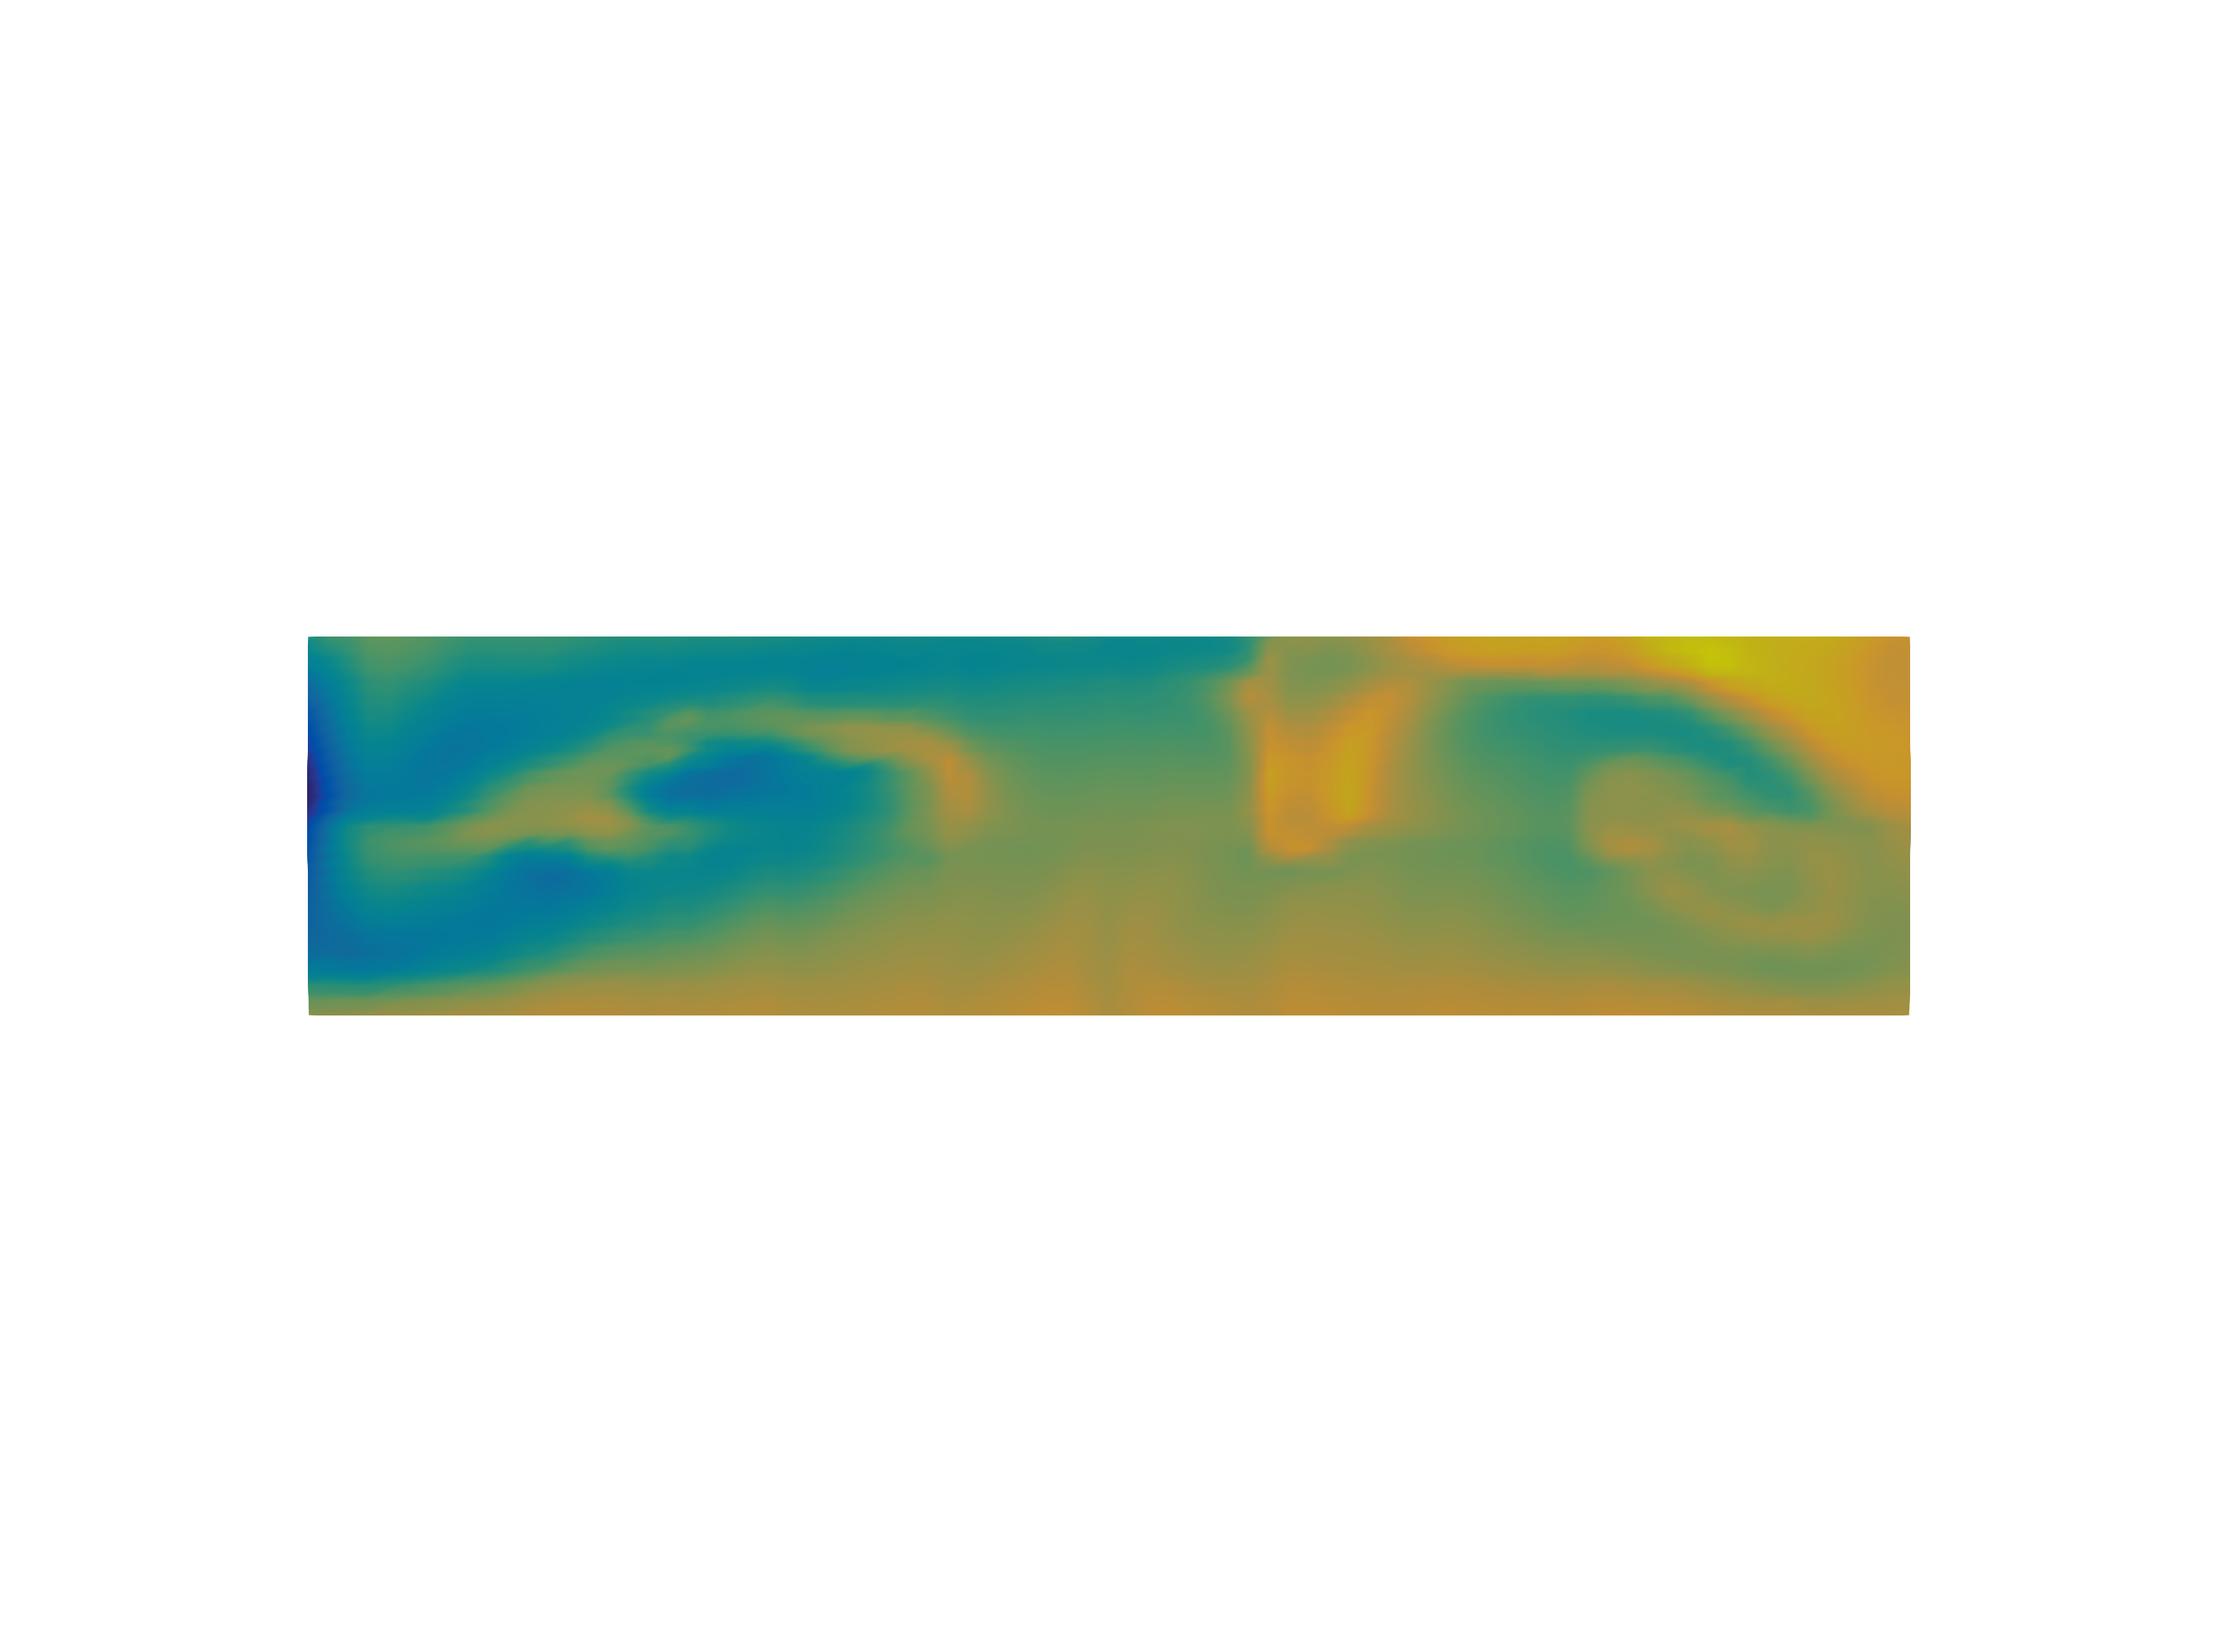
\includegraphics[width=\rasterimagewidth]{{../media/populations/application/print/alumina-influance-heaviside-2.55-3.08}.png}}};
        \end{axis}
      \end{tikzpicture}
      \begin{tikzpicture}
        \begin{axis}[
            colorbar,
            hide axis,
            scale only axis,
            height=0.41\rasterimagewidth,,
            width=\rasterimagewidth,
            colorbar horizontal,
            point meta min=2.55,
            point meta max=3.08,
            colorbar style={
              title=Concentration [\%w],
              width=7.4cm,
              height=0.3cm,
              xtick={2.5,2.55,2.75, 3,3.08, 3.5, 4, 4.5, 5, 5.5, 6},
              at={(0.5\rasterimagewidth,0.4cm)},
              anchor=north
            }
          ]
          \addplot [] coordinates {(0,0)};
          \node (myfirstpic) at (0,0) {\framebox{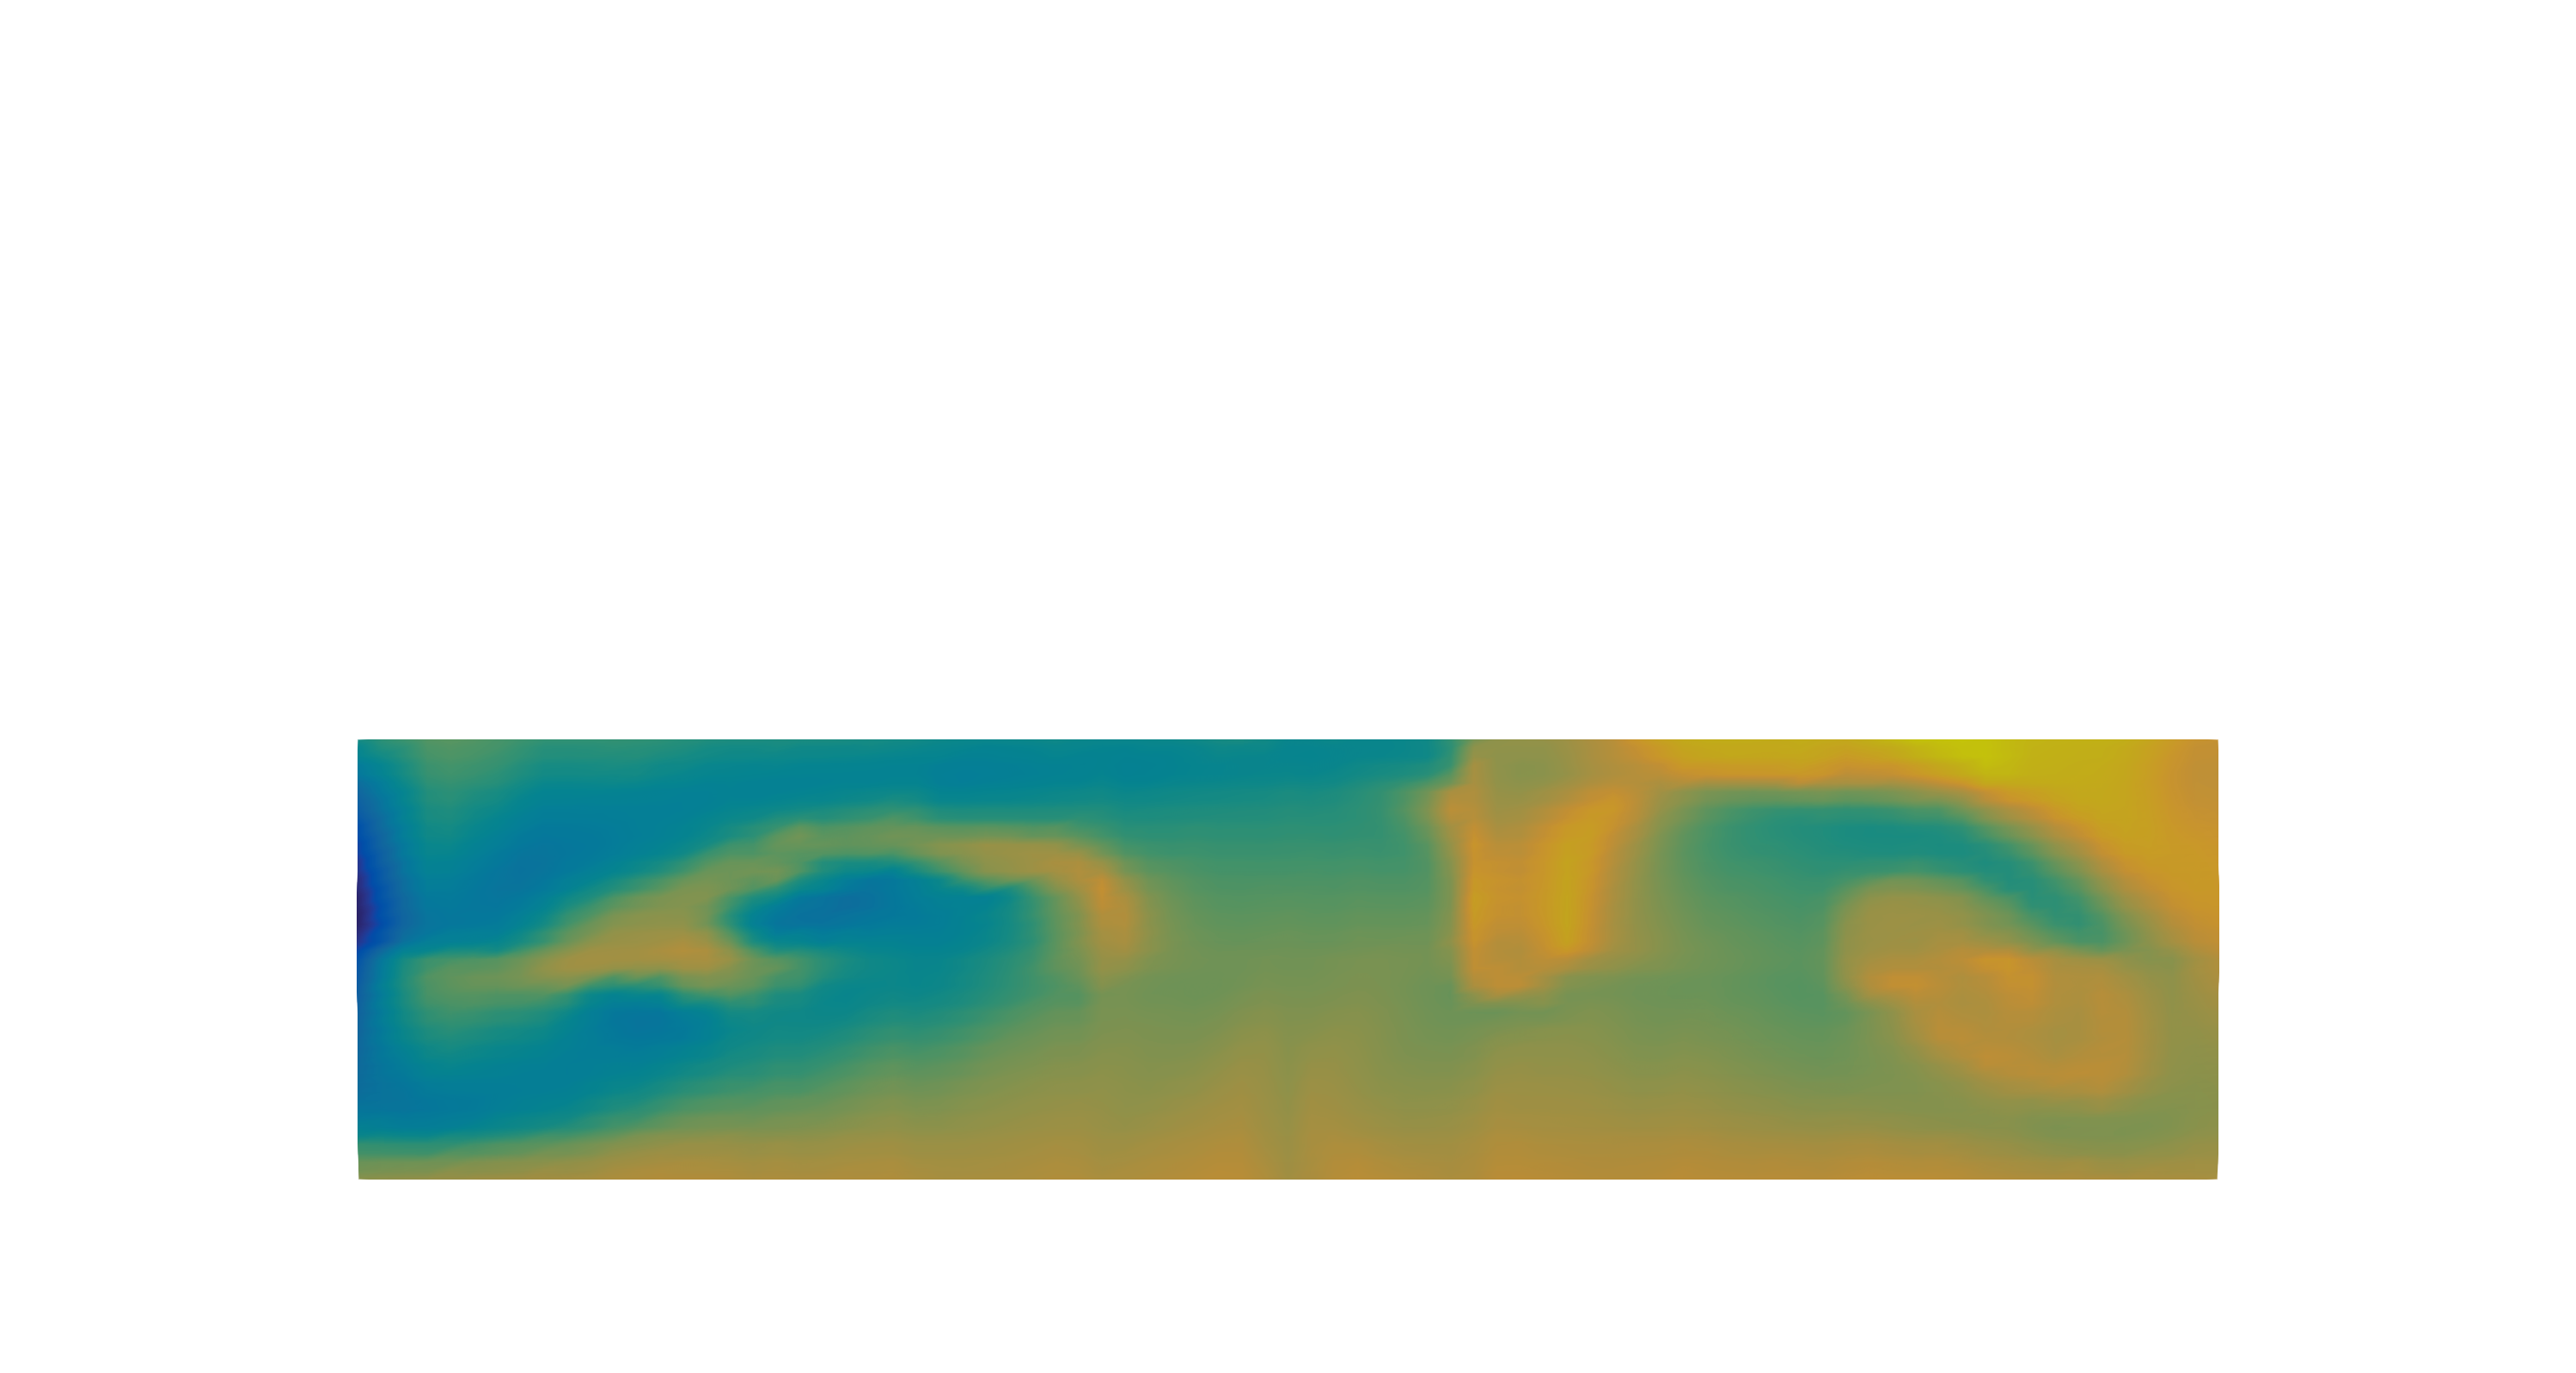
\includegraphics[width=\rasterimagewidth]{{../media/populations/application/print/alumina-influance-exp-2.55-3.08}.png}}};
        \end{axis}
      \end{tikzpicture}
    \caption{Champ de concentration $c$ dans l'ACD de la cuve AP32 à
      $t = $ \num{10000} \si{\second}. En haut, $T_\text{Crit} =
      T_\text{Liq}$. En bas, $T_\text{Crit} = T_\text{Liq} + 0.86$
      \si{\kelvin}.}
    \label{fig:dissolution-influence-exp-heaviside}
  \end{center}
\end{figure}


Dans la limite où $\tcrit - \tliq$ devient grand, on voit facilement
dans l'expression (\ref{eq:dissolution-rate}) que le taux de
dissolution des particules, et donc leur vitesse de dissolution,
devient nulle dans l'intervalle de température que le bain
électrolytique peut raisonnablement admettre. Par conséquent, si la
valeur de $\tcrit - \tliq$ est trop élevée, le temps dissolution des
particules peut devenir arbitrairement long, ce qui n'est pas réaliste
dans le cas d'une cuve d'électrolyse d'aluminium industrielle.

A l'inverse, en prenant la limite $\tcrit \to  \tliq$, le taux de
dissolution (\ref{eq:dissolution-rate}) s'écrit:
\begin{equation}\label{eq:dissolution-rate-zero-tcrit}
  \dissolutionrate(\concentration,\temperature) = \left\{
  \begin{array}{ll}
  K \displaystyle\frac{\csat - \concentration}{\csat}& \text{ si } \temperature
  \geq \tliq\text{ et } 0\leq \concentration \leq \csat,\\
  0 &  \text{ sinon.}
  \end{array}
  \right.
\end{equation}
En d'autres termes, la dissolution des particules est contrôlée
uniquement par la concentration locale $\concentration$ si
$\temperature \geq \tliq$, et ne se dissolvent pas sinon.

Nous présentons maintenant la distribution de concentration d'alumine
dissoute dans le bain de la cuve AP32 dans l'état stationnaire
périodique résultant de deux calculs. Comme précédemment, l'ensemble
des paramètres du modèle de transport et dissolution est reporté dans
la table \ref{tab:dissolution-physical-parameters}. Pour le premier
calcul on fixe $\tcrit = \tliq$, et le taux de dissolution est donné par
(\ref{eq:dissolution-rate-zero-tcrit}). Pour le deuxième calcul on
fixe $\tcrit = \tliq + 0.86$ \si{\kelvin}.

La figure \ref{fig:dissolutions-influence-exp-heaviside}
présente la concentration d'alumine dans l'ACD de la cuve AP32 à $t =
\num{10000}$ \si{\second}, lorsque l'état stationnaire périodique est
atteint. Le premier champ de concentration correspond au cas où
$\tcrit = \tliq$, tandis que le deuxième champ de concentration
correspond au cas où $\tcrit = \tliq + 0.86$ \si{\kelvin}. Même si
l'on parvient à observer de petites variations entre ces deux
solutions, en particulier dans le coin aval droite et autour du point
d'injection \#4, ces deux champs de concentration sont indistinguables
l'un de l'autre.

Finalement, nous nous penchons sur l'effet de la chute
gravitationnelle des particules d'alumine sur le champ de
concentration d'alumine dissoute.

% Sensibilité par rapport a la vitesse de chute dans le bain
\paragraph{Effet de la vitesse de chute des particules sur leur
  dissolution}
\begin{figure}[!hp]
  \begin{center}
      \begin{tikzpicture}
        \begin{axis}[
            hide axis,
            %colorbar,
             scale only axis,
             height=0.41\rasterimagewidth,,
             width=\rasterimagewidth,
             %colorbar horizontal,
             point meta min=2.38,
             point meta max=4.21,
             colorbar style={
               title=Concentration [\%w],
               width=7.4cm,
               height=0.3cm,
               xtick={2.38, 3, 3.5, 4,4.21, 4.5, 5, 5.5, 6},
               at={(0.5\rasterimagewidth,0.4cm)},
               anchor=north
            }
          ]
          \addplot [] coordinates {(0,0)};
          \node (myfirstpic) at (0,0) {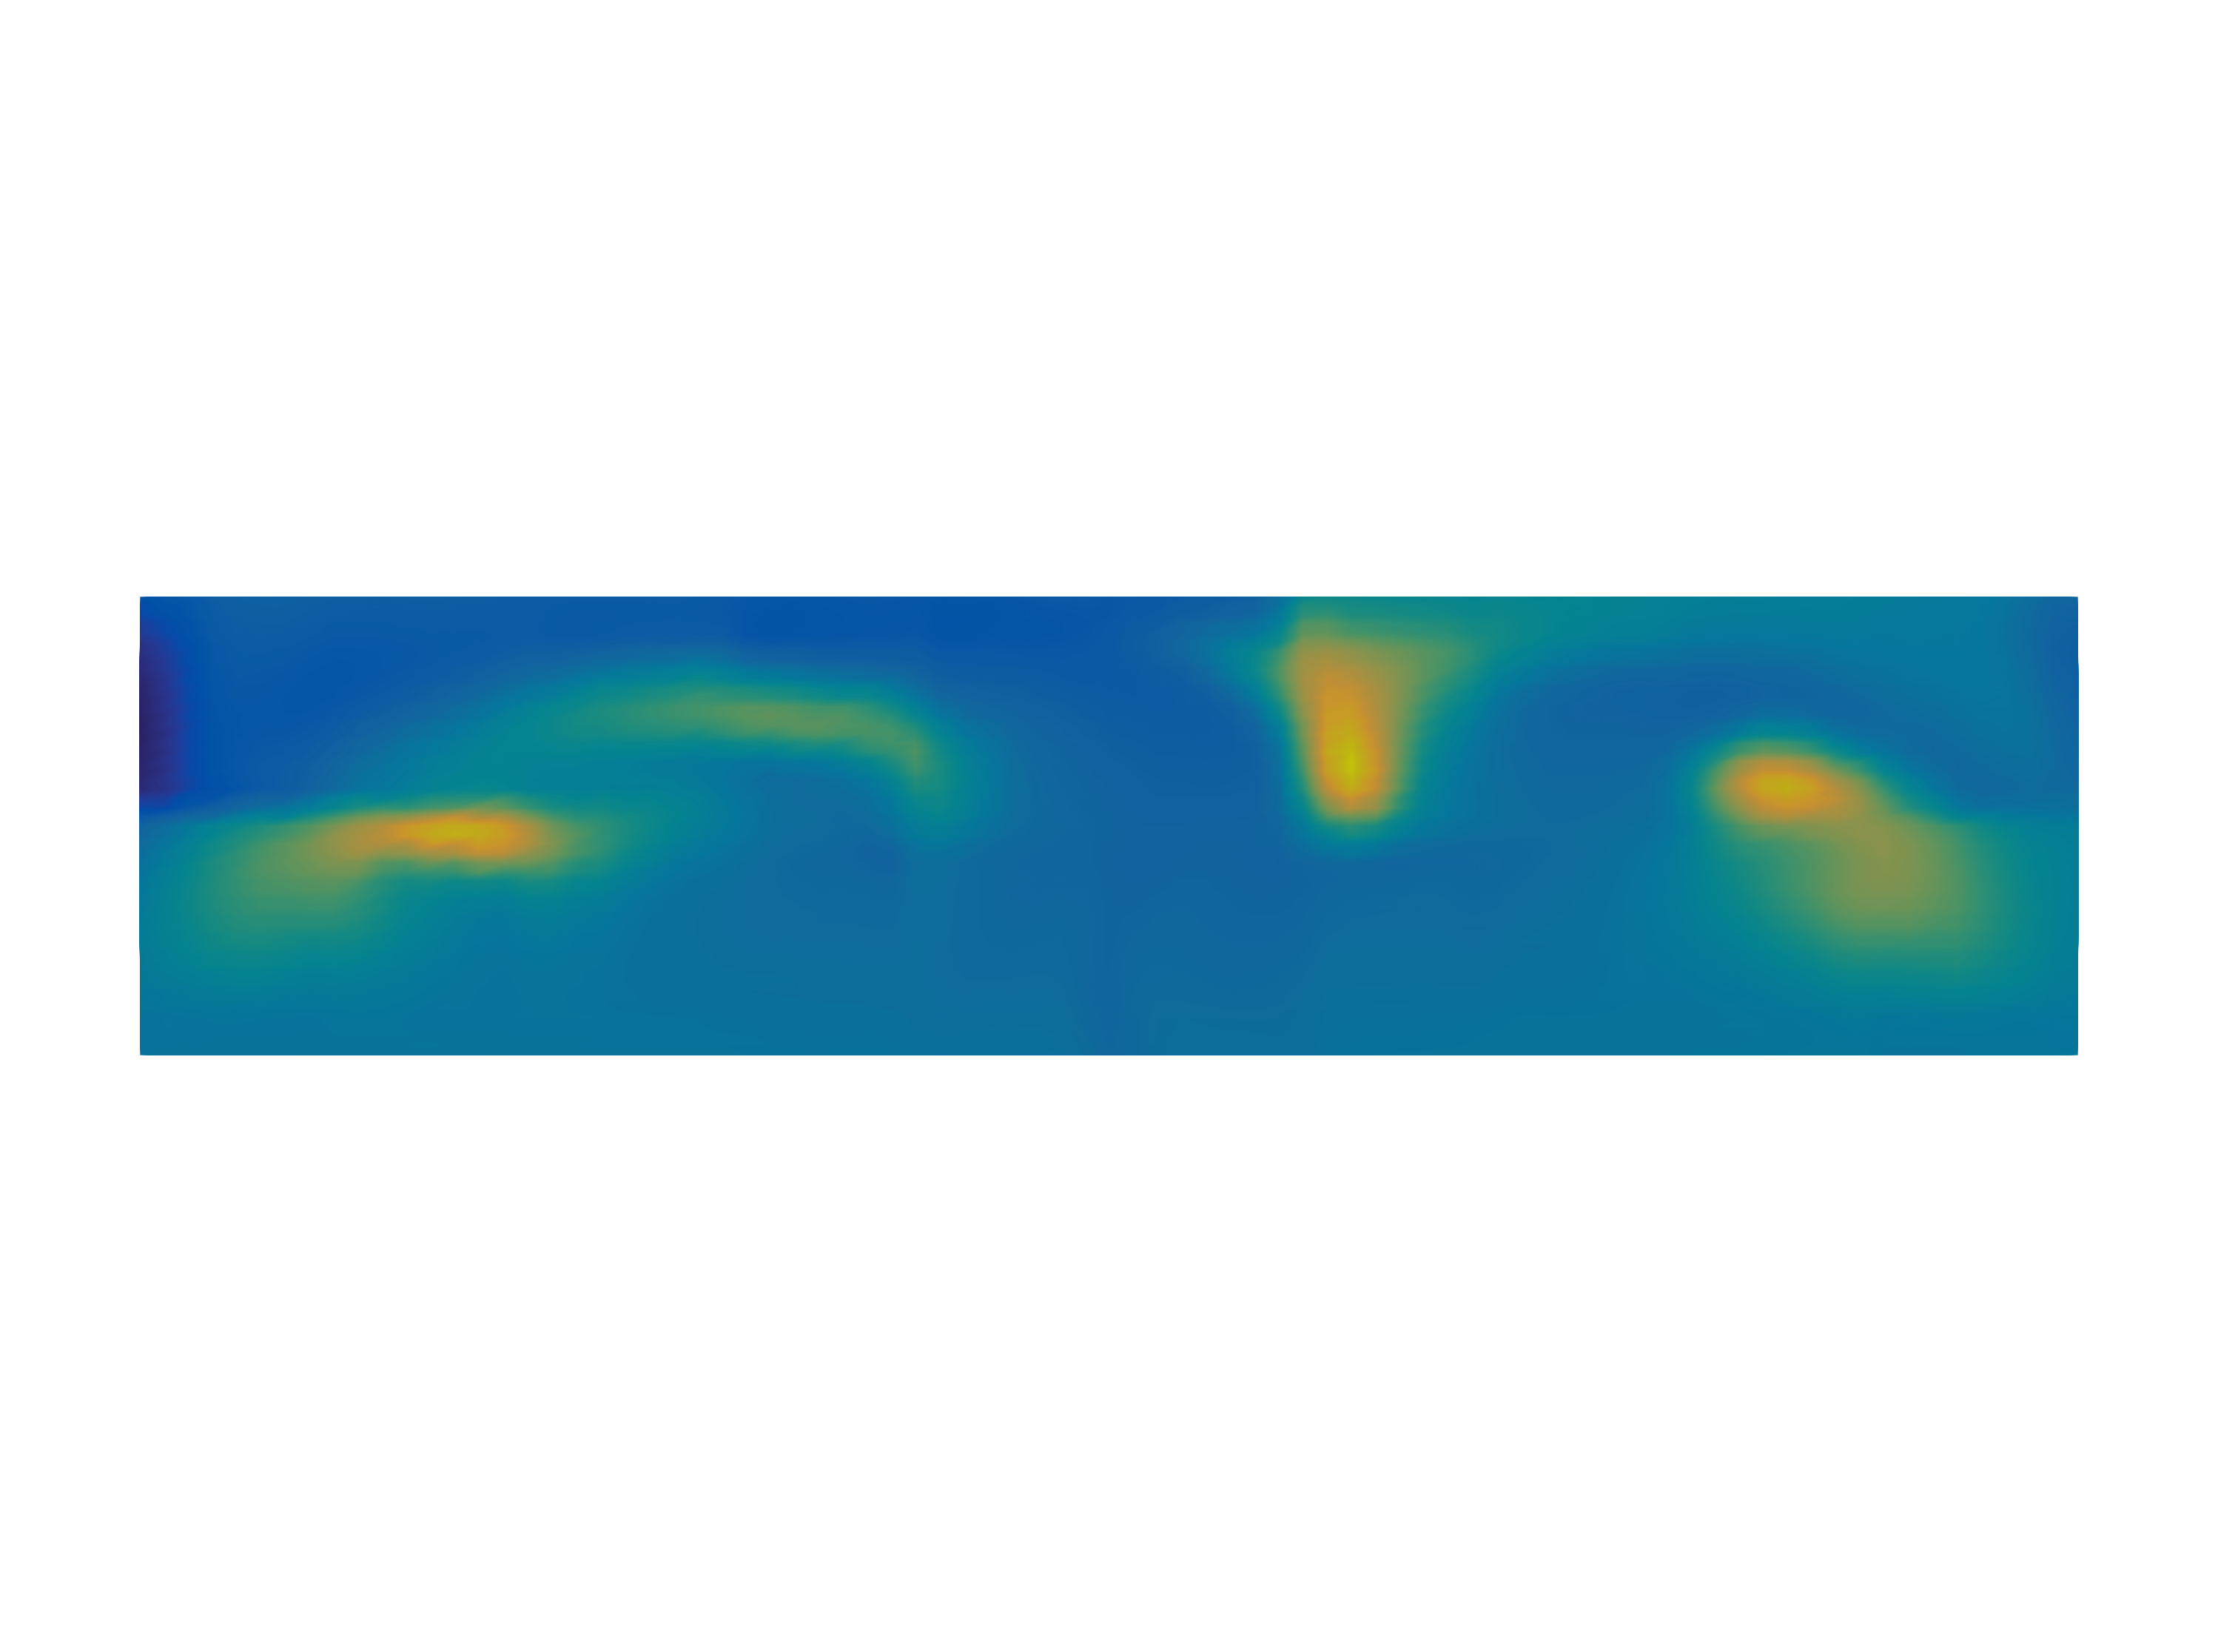
\includegraphics[width=\rasterimagewidth]{{../media/populations/application/print/alumina-control-2.38-4.21}.png}};
        \end{axis}
      \end{tikzpicture}
      \begin{tikzpicture}
        \begin{axis}[
            colorbar,
            hide axis,
            scale only axis,
            height=0.41\rasterimagewidth,
            width=\rasterimagewidth,
            colorbar horizontal,
            point meta min=2.38,
            point meta max=4.21,
            colorbar style={
              title=Concentration [\%w],
              width=7.4cm,
              height=0.3cm,
              xtick={2.38, 3, 3.5, 4,4.21, 4.5, 5, 5.5, 6},
              at={(0.5\rasterimagewidth,0.4cm)},
              anchor=north
            }
          ]
          \addplot [] coordinates {(0,0)};
          \node (myfirstpic) at (0,0) {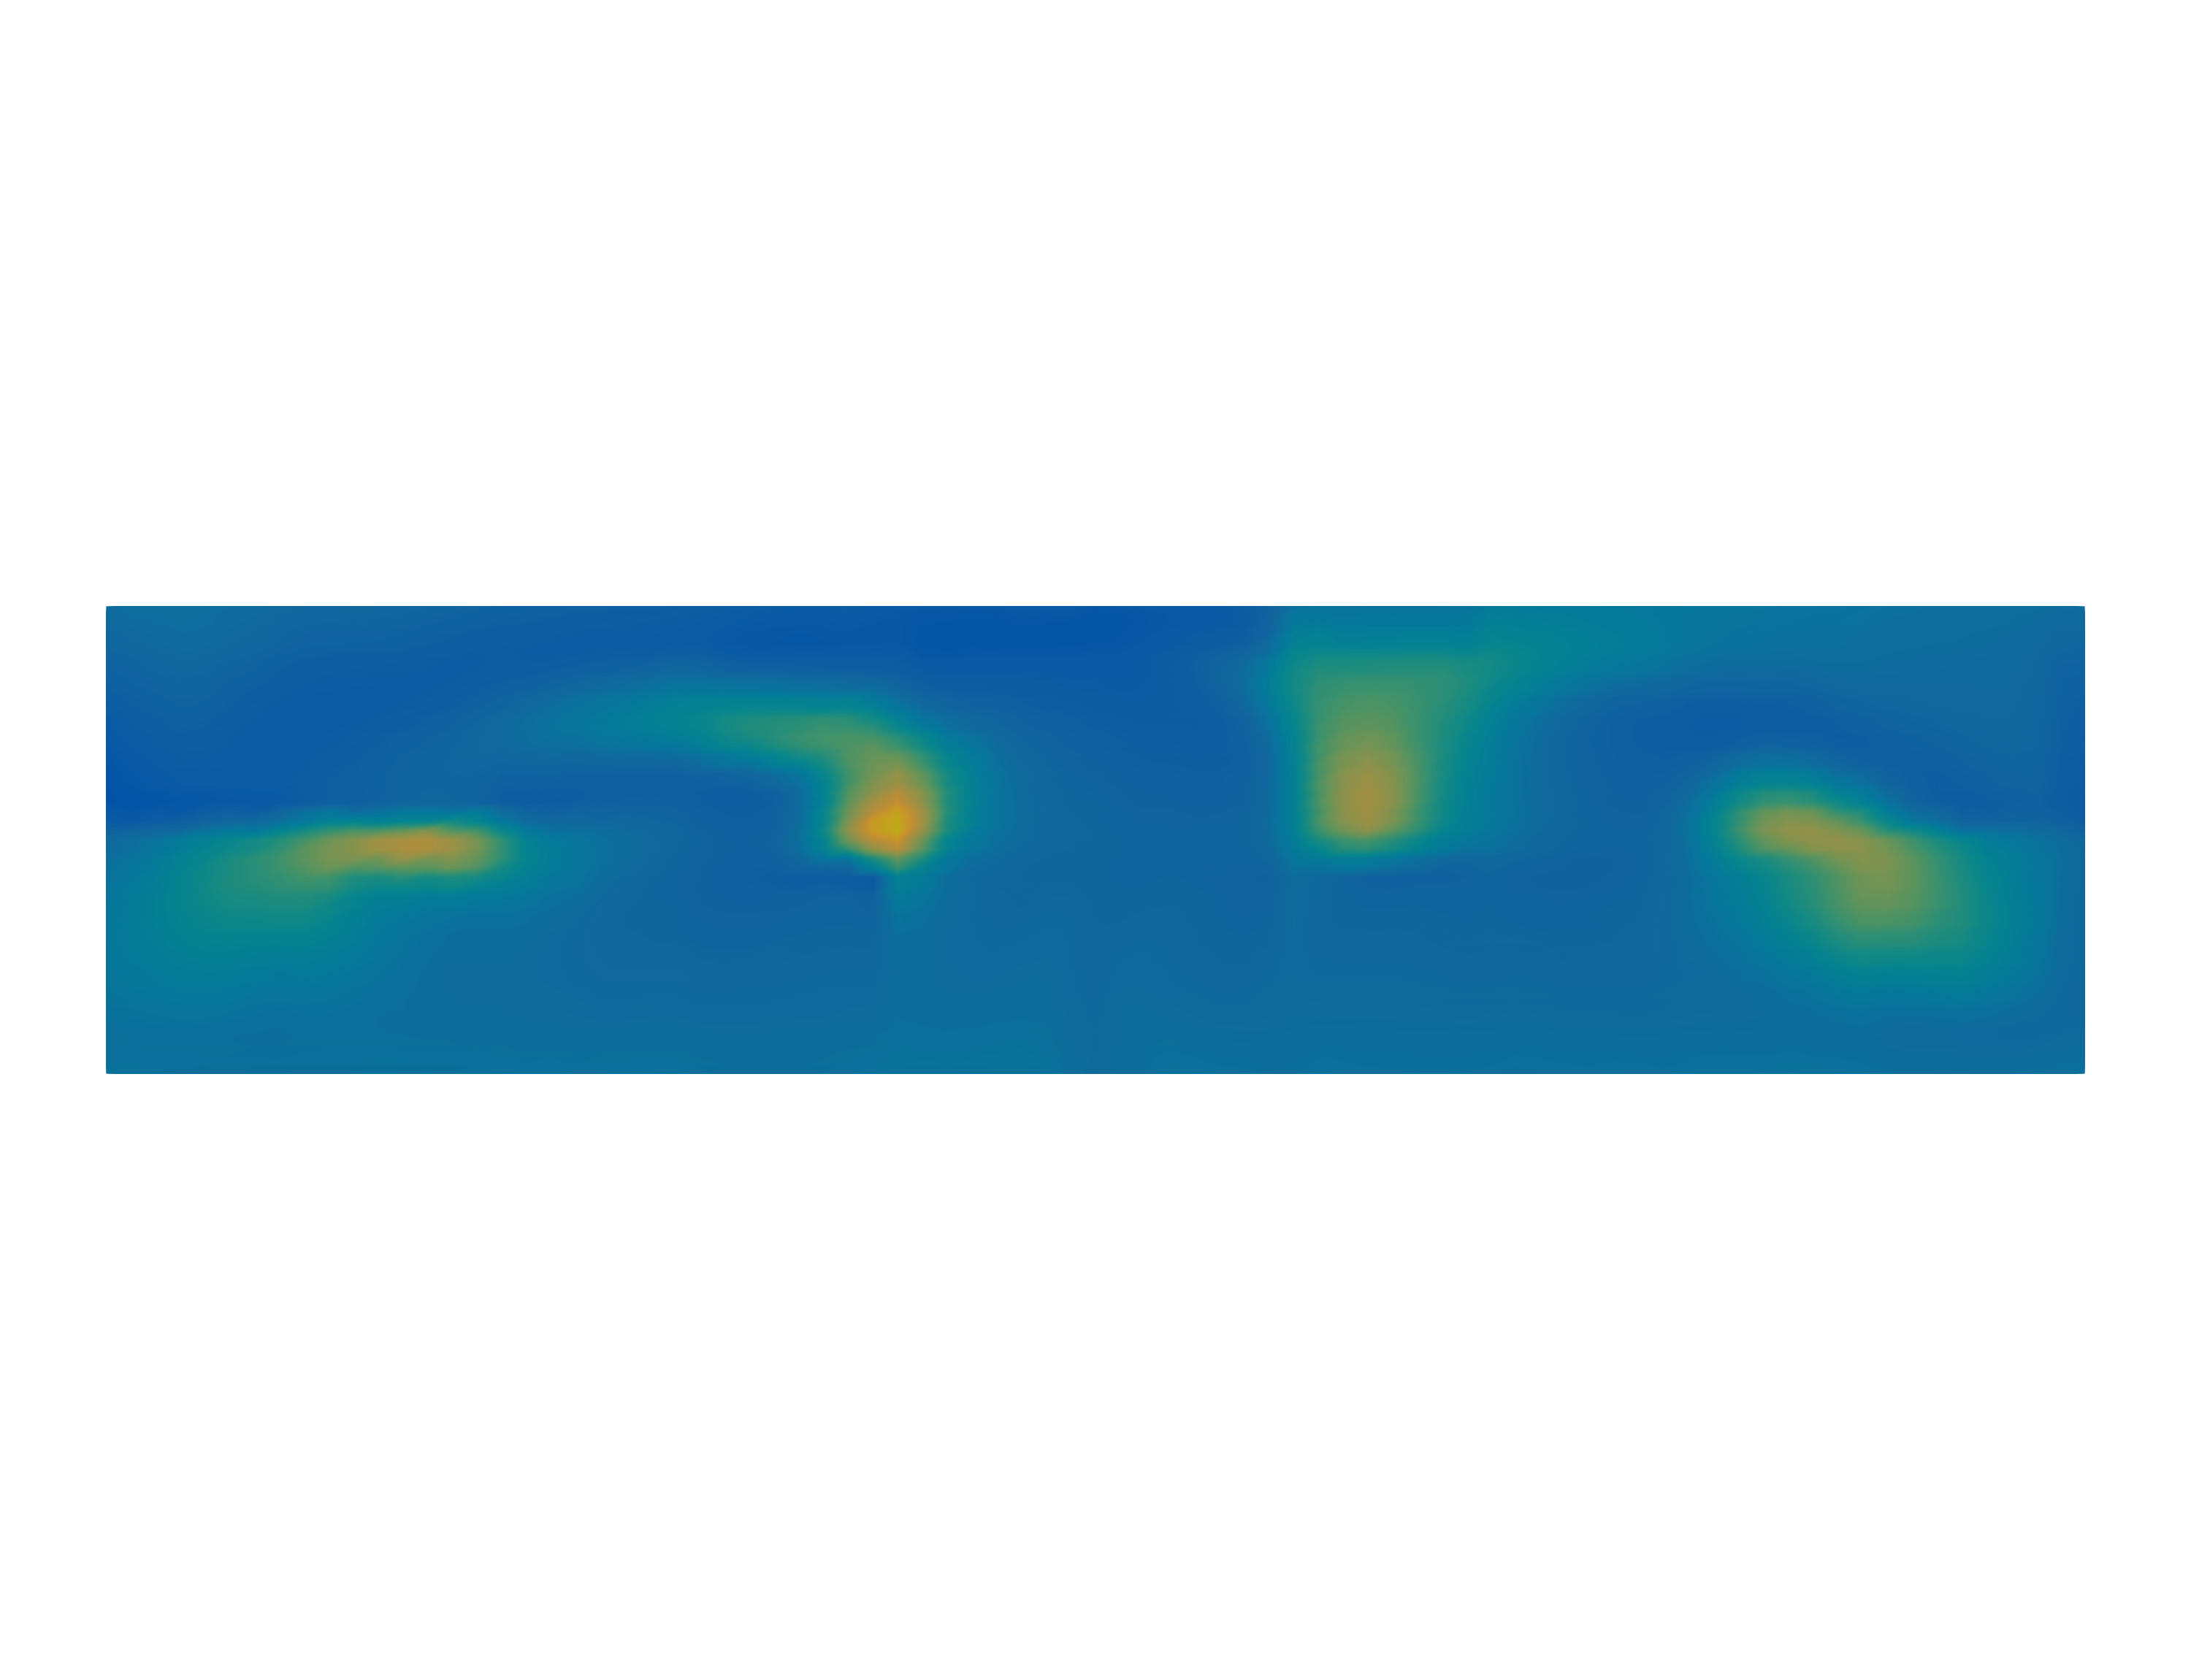
\includegraphics[width=\rasterimagewidth]{{../media/populations/application/print/dummy-tmp-result-c-2.38-4.21}.png}};
        \end{axis}
      \end{tikzpicture}
      \caption{Champ de concentration d'alumine dissoute dans l'ACD de
        la cuve AP32 à $t = \num{10000}\si\second$. En haut,
        dissolution des particules sans chute gravitationnelle dans le
        bain. En bas, dissolution des particules avec chute
        gravitationnelle dans le bain.}
      \label{fig:sedimentation-comparaison}
  \end{center}
\end{figure}


Nous avons déterminé, dans la section \ref{sec:particle-fall}, vitesse
de chute et la profondeur maximale atteinte dans le fluide de
particules soumisent à la gravité et à une force de traînée de
Stokes. Dans le cas le plus favorable, les particules de plus grande
taille peuvent chuter de plusieurs centimètres dans le bain
électrolytique avant de se dissoudre complètement.

Dans ce dernier paragraphe, nous proposons de comparer deux calculs
qui illustrent l'effet de la chute des particules dans le bain sur la
concentration d'alumine dissoute dans celui-ci.

Pour le premier calcul, qui joue le rôle de point de référence, les
paramètres sont reporté dans la table
\ref{tab:dissolution-physical-parameters} et nous annulons
l'accélération de la gravité $g = 0$, ce qui donne lieu à une vitesse
de chute strictement nulle, soit $w(r) = 0$ pour tout $r>0$. De plus,
l'injection des dose d'alumine a lieu dans le canal central comme
indiqué sur la figure \ref{fig:injections}, au niveau de l'ACD.

Pour le deuxième calcul la valeur de $g$ est restaurée, telle que
donnée dans la table \ref{tab:dissolution-physical-parameters} et la
vitesse de chute des particules est donnée par l'expression
\ref{eq:fall-velocity}. Cependant, les points d'injections sont
déplacés verticalement vers le haut du canal.

Nous avons montré dans la section \ref{sec:particle-fall} que les
profondeurs maximales atteintes par les particules lorsque la viscosité
du fluide est supérieure ou égale à \num{1e-2}
\si{\kilo\gram\per\meter\per\second} sont de l'ordre du
millimètre. Or, la taille verticale des mailles dans les canaux ne
permet pas de capturer des effets de cette amplitude. Pour cette
raison, nous choisissons pour le paramètre de viscosité
$\electrolyteviscosity$, qui intervient dans la définition
(\ref{eq:fall-velocity}), la viscosité laminaire du fluide, soit
$\electrolyteviscosity = $ \num{2e-3}
\si{\kilo\gram\per\meter\per\second}. Cette valeur de la viscosité
donne lieu à des profondeurs de chute maximale de particule dans le
bain de l'ordre de quelques centimètres.

La figure \ref{fig:sedimentation-comparaison} représente les champs de
concentration dans l'ACD de la cuve AP32 obtenus par ces deux calculs,
évalué à $t = \num{10000}$ \si{\second}, lorsque l'état stationnaire
périodique est atteint.

On remarque quelques différences entre les deux solutions,
essentiellement au niveau des points d'injection. Les valeur maximales
de la concentration d'alumine dissoute à proximité des points
d'injection \#1, \#3 et \#4 sont plus grandes lorsque lorsque la chute
des particules est négligée. On constate l'effet inverse pour
l'injecteur \#2: la concentration d'alumine dissoute sous cet
injecteur atteint un maximum local plus marqué lorsque la chute des
particules est pris en compte. Dans le reste du bain, la distribution
de concentration est similaire entre les deux calculs.

Nous concluons cette partie par une discussion de ces résultats.
